\documentclass[12pt]{article}
\textwidth 16.5cm
\textheight 23.5cm
\oddsidemargin 0pt
\topmargin -2cm
\usepackage{epsf}
%\usepackage{enumerate}
%\usepackage{natbib}
%\usepackage{url} % not crucial - just used below for the URL 

%\pdfminorversion=4
% NOTE: To produce blinded version, replace "0" with "1" below.



%\setlength{\parindent}{.3in}
%\setlength{\parskip}{.05in}
\usepackage{latexsym,amsmath,amssymb,amsfonts,amsthm,bbm,mathrsfs,breakcites,dsfont,xcolor}
\usepackage{stmaryrd,epsf}
\usepackage{natbib}
\bibliographystyle{abbrvnat}

\setcitestyle{authoryear, open={(},close={)}}
\usepackage{soul}
\usepackage{url}
\usepackage{dsfont}
\usepackage{enumerate}
\usepackage{graphicx}
\usepackage{graphics}
\usepackage{psfrag}
\usepackage{caption, subcaption}
\usepackage{multirow}
%\usepackage{algorithm}
\usepackage[ruled,vlined]{algorithm2e}

% \usepackage[backend = biber, natbib,
    % style = authoryear]{biblatex}

%\usepackage{comment}
%\newcommand{\indep}{\rotatebox[origin=c]{90}{$\models4[]}
\usepackage[colorlinks,linkcolor=black,citecolor=blue,urlcolor=blue,breaklinks = true]{hyperref}

\newtheorem{theorem}{Theorem}
\newtheorem{lemma}[theorem]{Lemma}
%\newtheorem{example}[]{Example}
\newtheorem{proposition}[theorem]{Proposition}
\newtheorem{corollary}[theorem]{Corollary}
\newtheorem{assumption}{A\!\!}
\newtheorem{example}{Example}

\DeclareMathOperator*{\argmax}{arg\,max}
\DeclareMathOperator*{\argmin}{arg\,min}
% \renewcommand{\baselinestretch}{1.25}
\newcommand{\indep}{\rotatebox[origin=c]{90}{$\models$}}
\newcommand{\red}[1]{\textcolor{red}{#1}}
\newcommand{\blue}[1]{\textcolor{blue}{#1}}
\newcommand{\green}[1]{\textcolor{green}{#1}}
\newcommand{\orange}[1]{\textcolor{orange}{#1}}
\newcommand{\var}{\mathrm{Var}}
\newcommand{\cov}{\mathrm{Cov}}
\newcommand{\bbE}{\mathbb{E}}

\usepackage{xcolor}
\usepackage[draft,inline,nomargin,index]{fixme}
\fxsetup{theme=color,mode=multiuser}
\FXRegisterAuthor{tc}{atc}{\color{red} TC}
\FXRegisterAuthor{jb}{abc}{\color{green} JB}

\usepackage[acronym, toc]{glossaries}


\makeglossaries 

\newacronym{lasso}{LASSO}{Least Absolute Shrinkage and Selection Operator}
\newacronym{tmb}{TMB}{Tumour Mutation Burden}
\newacronym{tib}{TIB}{Tumour Indel Burden}
\newacronym{icb}{ICB}{Immune Checkpoint Blockade}
\newacronym{ici}{ICI}{Immune Checkpoint Inhibitor}
\newacronym{msi}{MSI}{Micro-Satellite Instability}
\newacronym{ctla4}{CTLA-4}{Cytotoxic T Lymphocyte Associated protein 4}
\newacronym{pdl1}{PD-L1}{Programmed Death Ligand 1}
\newacronym{wes}{WES}{Whole Exome Sequencing}
\newacronym{ctdna}{ctDNA}{Circulating Tumour DNA}
\newacronym{bmr}{BMR}{Background Mutation Rate}
\newacronym{nsclc}{NSCLC}{Non-Small Cell Lung Cancer}
\newacronym{auprc}{AUPRC}{Area Under Precision-Recall Curve}
\newacronym{ectmb}{ecTMB}{Estimation and Classification of Tumour Mutation Burden}

\title{Data-driven design of targeted gene panels for estimating immunotherapy biomarkers}
 \author{Jacob R. Bradley and Timothy I. Cannings
 \\ \emph{School of Mathematics, University of Edinburgh}}
\date{}
\begin{document}


\maketitle
\begin{abstract}
We introduce a novel data-driven framework for the design of targeted gene panels for estimating exome-wide biomarkers in cancer immunotherapy. Our first goal is to propose a generative model for the profile of mutation across the exome, which allows for gene- and variant type-dependent mutation rates. Based on this model, we then develop a new procedure for estimating biomarkers such as \acrlong{tmb} and \acrlong{tib}.  Our approach allows the practitioner to construct a targeted gene panel of a prespecified size, alongside an estimator that only depends on the selected genes, which facilitates cost-effective prediction.  Alternatively, the practitioner may apply our method directly to an existing gene panel. We demonstrate the excellent performance of our proposal using an annotated mutation dataset from 1144 \acrlong{nsclc} patients. 

%Our approach is based on a generative model for the profile of mutation across the exome, which allows for gene- and variant type-dependent mutation rates.  We then develop a new estimation procedure for constructing estimators of biomarkers.

%\tcnote{which data?}
%\jbnote{is our procedure for estimating biomarkers or producing estimators?}

 %Our method is flexible in that the same procedure and generative model can be used to produce estimators for different biomarkers. It also allows predictions based not just on the number but the type of mutations occurring in the genes of a panel. We provide error estimates for our procedure, and compare its performance against a variety of state-of-the-art methods, as well as gene panels from the literature. \\
%is developed, which allows differing mutation rates for different genes and variant types. This architecture allows for prediction using genes upon which there is selective pressure, which have previously had to be discounted despite often being the most clinically relevant. Our generative model allows the construction of reliable linear estimators of tunable sparsity via a convex optimisation problem based on the group Lasso. Our method is flexible in that the same procedure and generative model can be used to produce estimators for different biomarkers. It also allows predictions based not just on the number but the type of mutations occurring in the genes of a panel. We provide error estimates for our procedure, and compare its performance against a variety of state-of-the-art methods, as well as gene panels from the literature. 

\textbf{Keywords: cancer, gene panel design, tumour indel burden, tumour mutation burden.}
\end{abstract}

%\printglossary[type=\acronymtype]

\section{Introduction}
It has been understood for a long time that cancer, a disease occurring in many distinct tissues of the body and giving rise to a wide range of presentations, is initiated and driven by the accumulation of mutations in a subset of a person's cells \citep{boveri_concerning_2008}.  Since the discovery of \acrfull{icb}\footnote{For this work, James Allison and Tasuku Honjo received the 2018 Nobel Prize for Physiology/Medicine \citep{ledford_cancer_2018}.}  \citep{ishida_induced_1992,leach_enhancement_1996},  there has been an explosion of interest in cancer therapies targeting immune response and \acrshort{icb} therapy is now widely used in clinical practice \citep{robert_decade_2020}.  \acrshort{icb} therapy works by targeting natural mechanisms (such as the proteins \acrfull{ctla4} and \acrfull{pdl1} \citep{buchbinder_ctla-4_2016}) to disengage the immune system. Inhibition of these `checkpoints' can promote a more aggressive anti-tumour immune response \cite{pardoll_blockade_2012}, and in some patients this leads to long-term remission \citep{gettinger_5-year_2019}. However \acrshort{icb} therapy is not always effective \citep{nowicki_mechanisms_2018} and may have adverse side-effects, thus determining which patients will benefit in advance of treatment is vital. 

%\acrshort{icb}s are antibodies that bind to proteins on the surface of immune cells. 
%These surface proteins are known as immune checkpoints, the two most widely targeted being \acrfull{ctla4} and \acrfull{pdl1} \citep{buchbinder_ctla-4_2016}. 
%Inhibition of immune checkpoints with these antibodies promotes a more aggressive immune response to cancer in some patients \citep{pardoll_blockade_2012}. 

%While very successful in many patients, there are more still for whom \acrshort{icb} therapy provides little clinical benefit. This fact, along with the high cost and significant side-effects of \acrshort{icb} therapy, make it important to develop means of predicting which patients will benefit.

Exome-wide prognostic biomarkers for immunotherapy are now well-established -- in particular, \acrfull{tmb} may be used to predict response to immunotherapy \citep{zhu_association_2019, cao_high_2019}.  \acrshort{tmb} is defined as the total number of (non-synonymous) mutations occurring throughout the tumour exome, and can be thought of as a proxy for how easily a tumour cell can be recognised as foreign by immune cells \citep{chan_development_2019}. However, the cost of measuring \acrshort{tmb} using \acrfull{wes} \citep{sboner_real_2011} currently prohibits its widespread use as standard-of-care. These sequencing costs, both financial and in terms of the time taken for results to be returned, are especially problematic in situations where high-depth sequencing is required, such as when utilising blood-based \acrfull{ctdna} from liquid biopsy samples \citep{gandara_blood-based_2018}. The same issues are encountered when measuring more recently proposed biomarkers such as \acrfull{tib} \citep{wu_tumor_2019,turajlic_insertion-and-deletion-derived_2017}, which only includes mutations of strong immunogenicity. There is, therefore, demand for cost-effective approaches to estimate these biomarkers \citep{fancello_tumor_2019, golkaram_interplay_2020}.

In this paper we propose a novel, data-driven method for biomarker estimation, based on a generative model of how mutations arise in the tumour exome.  More precisely, we model mutation counts as independent Poisson variables, where the mean number of mutations depends on the gene of origin and variant type, as well as the \acrfull{bmr} of the tumour. Due to the ultrahigh-dimensional nature of sequencing data, we use a regularisation penalty when estimating the model parameters, in order to reflect the fact that in many genes' mutations arise purely according to the \acrshort{bmr}. In addition, this identifies a subset of genes that are mutated above or below the background rate, which may be of clinical interest. Our model facilitates the construction of a new estimator of \acrshort{tmb}, based on a weighted linear combination of the number of mutations in each gene. The vector of weights is chosen to be sparse (i.e.~have many entries equal to zero), so that our estimator of \acrshort{tmb} may be calculated using only the mutation counts in a subset of genes. In particular, this allows for accurate estimation of \acrshort{tmb} from a targeted gene panel, where the panel size (and therefore the cost) may be determined by the user.  We demonstrate the excellent practical performance of our framework using a \acrfull{nsclc} dataset \citep{chalmers_analysis_2017}, including a comparison with the existing state-of-the-art data-driven approaches for estimating \acrshort{tmb}.   %Aside from its excellent performance at predicting \acrshort{tmb}, our method has a number of other benefits. 
Moreover, since our model allows variant type-dependent mutation rates, it can be adapted easily to predict other biomarkers, such as \acrshort{tib}. Finally, our method may also be used in combination with an existing targeted gene panel; we can estimate the biomarker directly from that panel, or first augment the panel and then construct an estimator.  % The fitted parameters of our model are interpretable and correspond to tangible biological effects and processes. We are also able to provide heuristic error bounds.

%It can be adapted very easily to predict \acrshort{tib}, due to our separately modelling mutations of different variant type.
%For estimating \acrshort{tmb} from a targeted gene panel, we are able to either select an optimal set of genes of a given total length, produce predictions from a pre-defined set of observed genes, or augment a pre-defined set of genes by a given amount of genomic space.

Due to the emergence of \acrshort{tmb} as a biomarker for immunotherapy in recent years, a variety of groups have considered methods for its estimation. A simple and common way to estimate \acrshort{tmb} is via the proportion of mutated codons in a targeted region. \citet{budczies_optimizing_2019} investigate how the accuracy of predictions made in this way are affected by the size of the targeted region, where mutations are assumed to occur at uniform rate throughout the genome. \citet{yao_ectmb_2020} modelled mutations as following a negative binomial distribution while allowing for gene-dependent rates, which are inferred by comparing nonsynonymous and synonymous mutation counts. In contrast, our method does not require data including synonymous mutations -- we can account for differences in mutation rate that affect synonymous and non-synonymous mutations, e.g.~chromatin configuration \citep{makova_effects_2015} and transcription-dependent DNA repair \citep{fong_intertwined_2013}.  Linear regression models have been used for both panel selection \citep{lyu_mutation_2018} and for biomarker prediction \citep{guo_exon_2020}. A review of some of the issues arising when dealing with targeted panel-based predictions of \acrshort{tmb} biomarkers is given by \citet{wu_designing_2019}. Finally, we are unaware of any methods for efficiently estimating \acrshort{tib}. 
% a more difficult task due to the low relative abundance of indel mutations and known reliability issues for sequencing genomic loci of highly repetitive nucleotide constitution \citep{narzisi_challenge_2015}.

The remainder of the paper is as follows. In Section \ref{sec:methodology}, we introduce our data sources, and provide a detailed description of our methodological proposal. Experimental results are given in Section~\ref{sec:experimentalresults}. \tcnote{Come back to this} We conclude in Section~\ref{sec:conclusion} with some remarks about our method's utility in the context of a wide span of literature around biomarker estimation, and future avenues for research.  Finally, we also provide an \texttt{R} package \texttt{ICBioMark} \citet{BradleyCannings_2020} which implements the methodology and reproduces the experimental results in the paper. 

 %we describe our generative model of mutation in Section~\ref{sec:genmodel} and show how regularised model fitting can allow us to infer a background mutation rate. In Section~\ref{sec:linearestimator} we show how to produce a sparse linear estimator via a convex optimisation based on the group \acrshort{lasso}. 

% At various points it is worth discussing possible biological interpretations that can be drawn from our results. 
% When this is not directly relevant to the question of biomarker estimation we leave these discussions for treatment in Appendices \ref{appendix:indelselection} and \ref{app:goodnessoffit}. Appendix \ref{app:errorbounds} contains formal derivations of expressions for error bounds.



\section{Methodology}
\label{sec:methodology}
\subsection{Data and terminology \label{sec:dataterminology}}
Our methodology can be applied to any annotated mutation dataset obtained by \acrshort{wes}. 
To demonstrate our proposal we make use of the \acrshort{nsclc} dataset produced by \citet{campbell_distinct_2016}, which contains data from 1144 patient-derived tumours.  For each sample in this dataset we have the genomic locations and variant types of all mutations identified.  The patients had a variety of prognoses and smoking histories, were aged between 39 and 90, and were approximately balanced by sex; see Figure~\ref{fig:1}. In Figure \ref{fig:2}A we see that mutations counts are distributed over a very wide range, as is the case in many cancer types \citep{chalmers_analysis_2017}. For simplicity, we only consider seven nonsynonymous variant types: missense mutations (which are the most abundant), nonsense mutations, frameshift insertions/deletions, splice site mutations, in-frame insertions/deletions, nonstop mutations and translation start site mutations.  We present the frequencies of these mutation types in Figure \ref{fig:2}B. Frameshift insertion/deletion (also known as indel) mutations are of particular interest when predicting \acrshort{tib}, but contribute only a small proportion ($<4\%$) of nonsynonymous mutations. 

\begin{figure}[htbp]
\centering
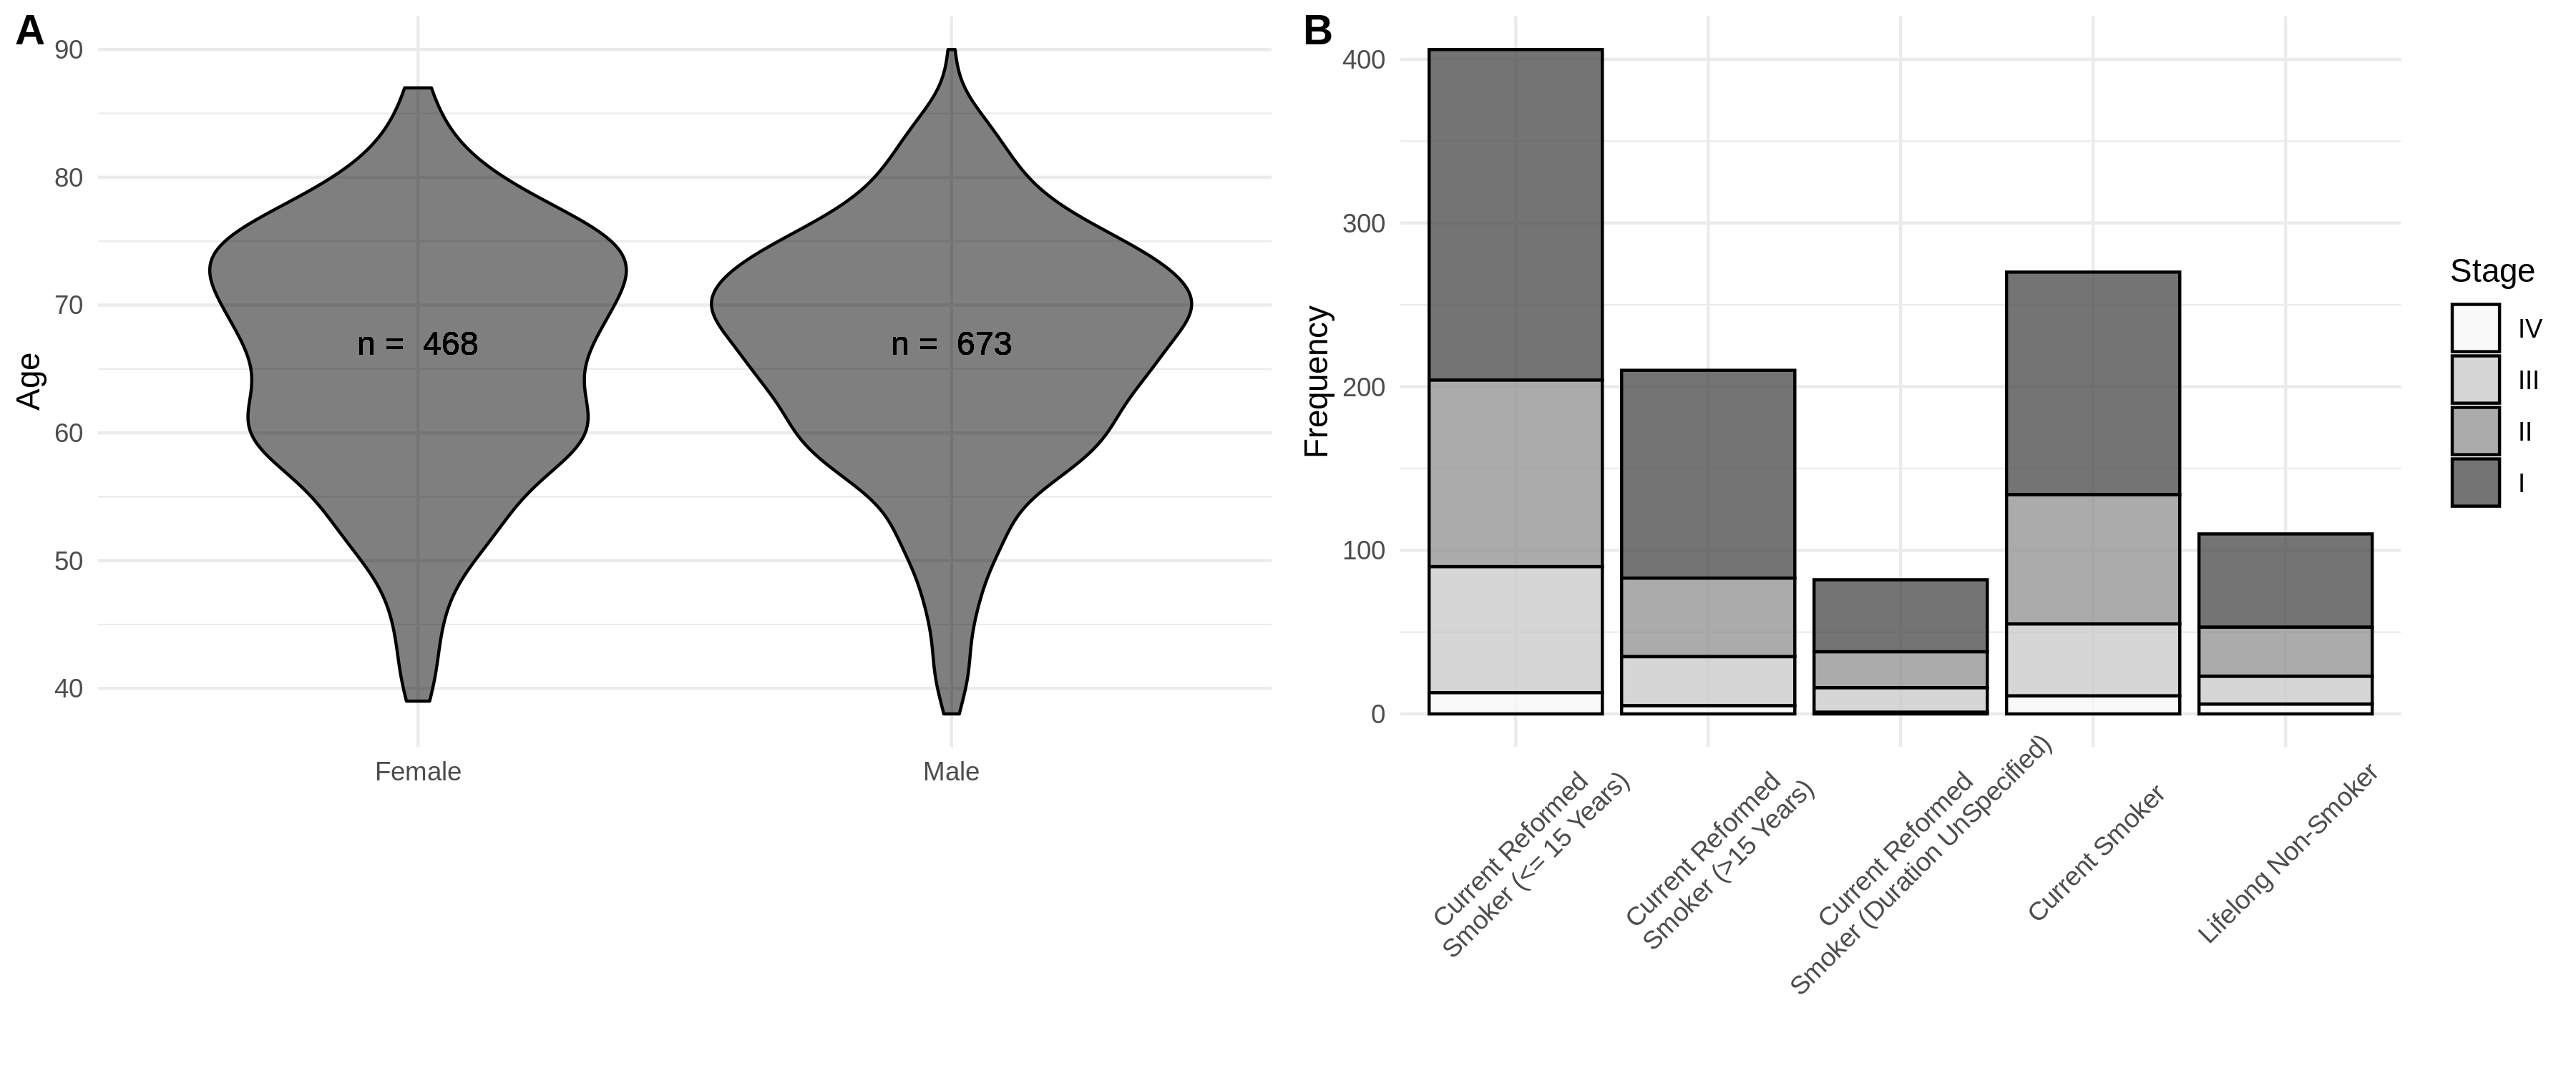
\includegraphics[width=6in]{figures/fig1.png}
\vspace*{-5mm}
\caption{Demographic data for the clinical cohort in \citet{campbell_distinct_2016}. \textbf{A}: Violin plots of age for patients, stratified by sex. \textbf{B}: Stacked bar chart of patients' smoking histories, shaded according to cancer stage diagnosis. \label{fig:1}}
\vspace*{-2mm}
\end{figure}

\begin{figure}[htbp]
\centering
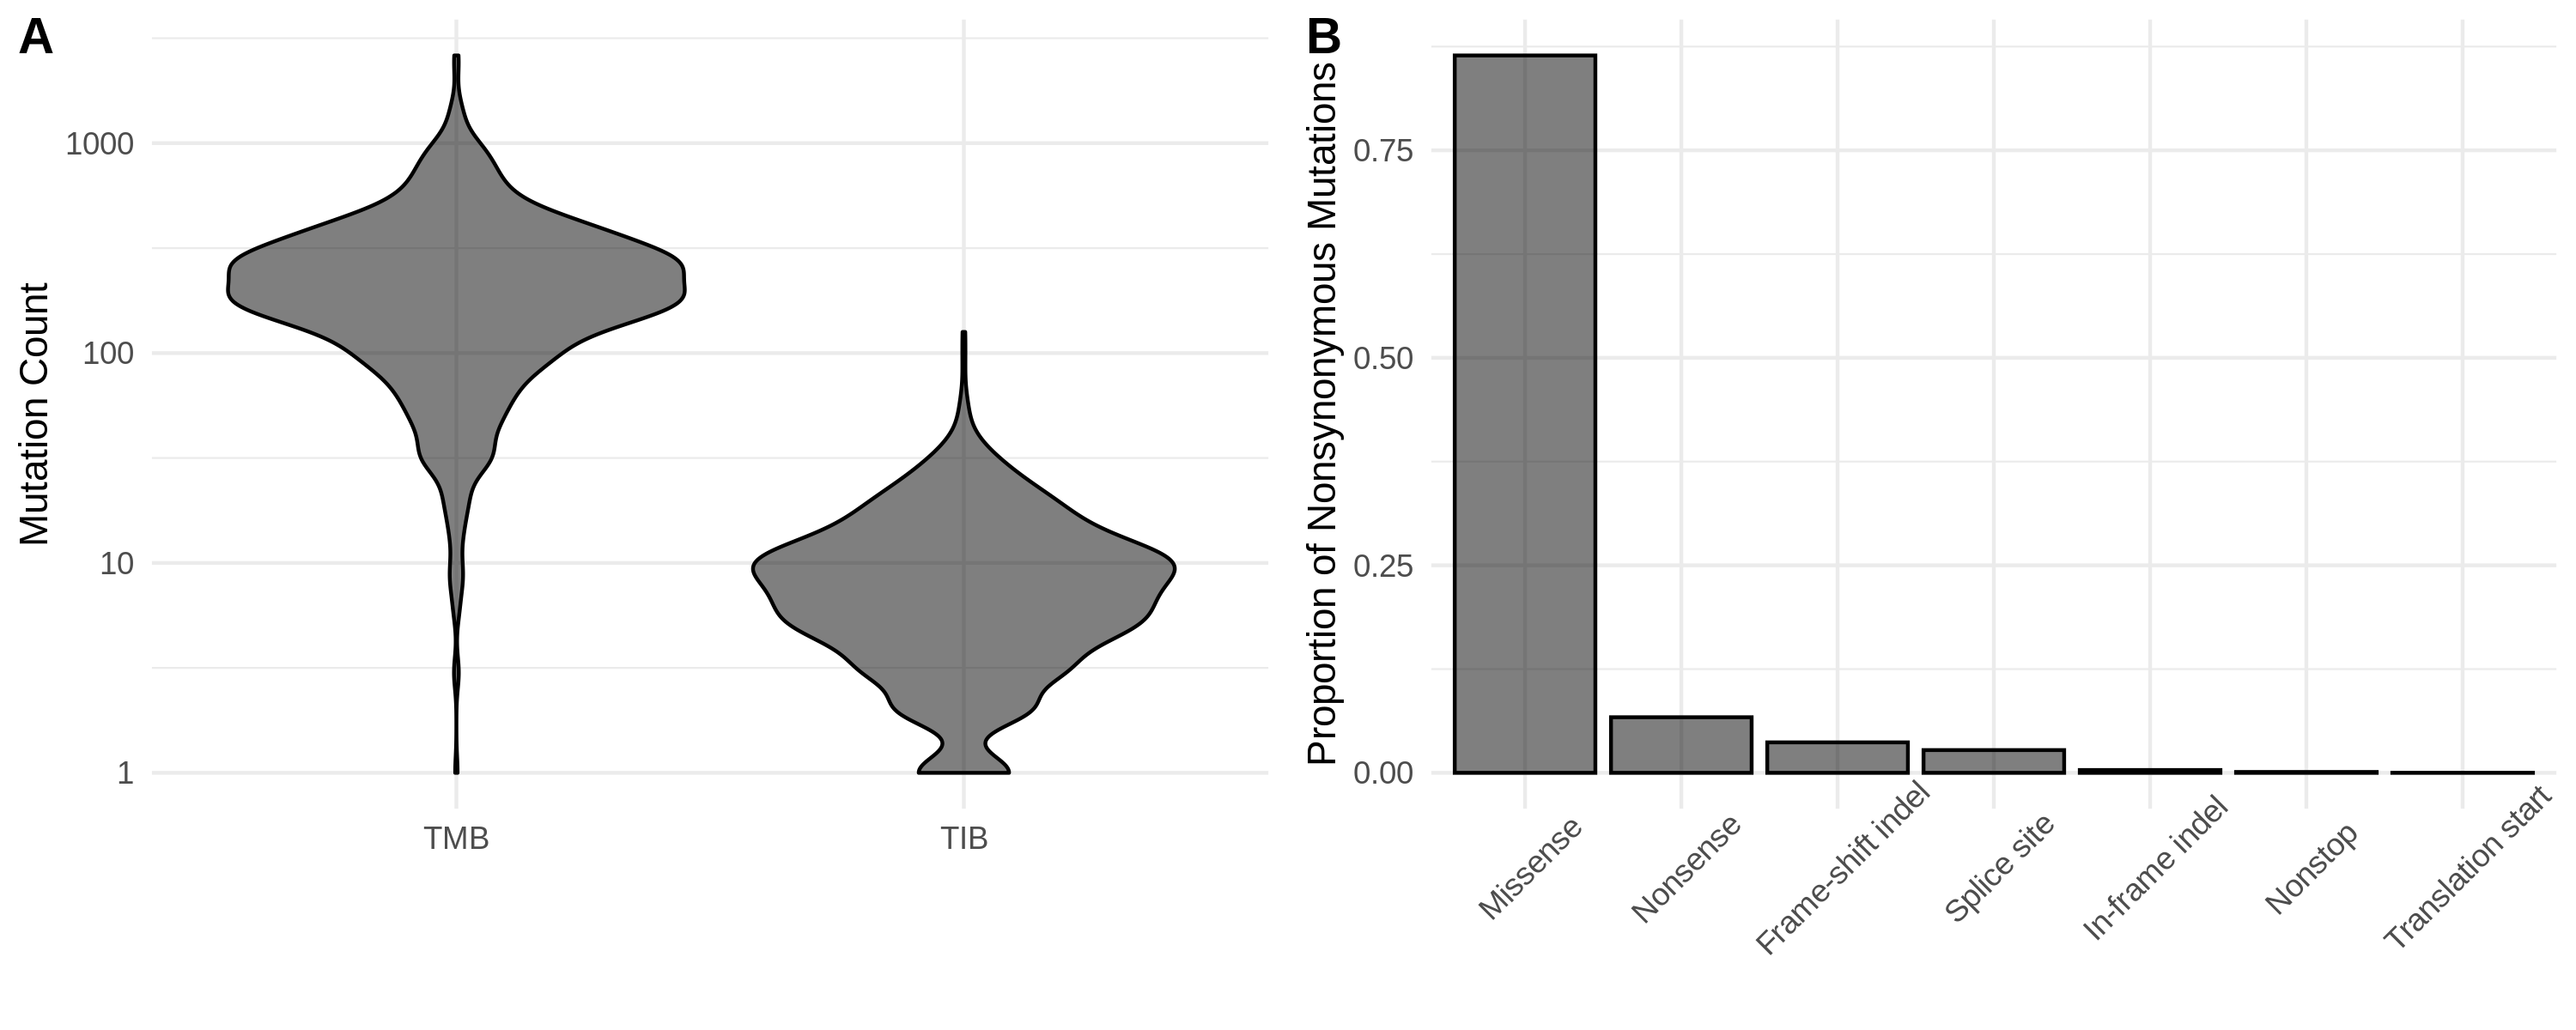
\includegraphics[width=6in]{figures/fig2.png}
\vspace*{-5mm}
\caption{ Dataset-wide distribution of mutations. \textbf{A}: Violin plot of the distribution of \acrshort{tmb} and \acrshort{tib} across training samples. \textbf{B}: The relative frequency of different nonsynonymous mutation types. \label{fig:2}}
\vspace*{-2mm}
\end{figure}

It is useful at this point to introduce the notation used throughout the paper. The set $G$ denotes the collection of genes that make up the exome. For a gene $g \in G$, let $\ell_g$ be the length of $g$ in nucleotide bases, defined by the maximum coding sequence\footnote{Maximum coding sequence is defined as the collection of codons that may be translated for some version of a gene, even if all the codons comprising the maximum coding sequence are never simultaneously translated. Gene coding lengths are extracted from the \emph{Ensembl} database \citep{yates_ensembl_2020}.}.  A gene panel is a subset $P \subseteq G$, and we write $\ell_P := \sum_{g \in P} \ell_g$ for its total length. We let $S$ denote the set of variant types in our data (e.g.~in the dataset mentioned above, $S$ contains the seven possible non-synonymous variants). Now, for $i = 0, 1, \ldots, n$, let $M_{igs}$ denote the count of mutations in gene $g \in G$ of type $s \in S$ in the $i$th sample. Here the index $i=0$ is used to refer to an unseen test sample for which we would like to make a prediction, while the indices $i=1,\ldots,n$ enumerate the samples in our training data set.  In order to define the exome-wide biomarker of particular interest, we specify a subset of mutation types $\bar{S} \subseteq S$, and let
\begin{equation}
T_{i\bar{S}} := \sum_{g \in G} \sum_{s \in \bar{S}} M_{igs},
\label{eq:biomarker}
\end{equation}
for $i=0,\ldots, n$.
% For example, if $\bar{S} = S$, i.e. the set of all non-synonymous mutation types in $S$, then $T_{i\bar{S}}$ is tumour mutation burden. Alternatively, if $\bar{S}$ contains only frameshift insertions and deletions, then $T_{i\bar{S}}$ refers to indel burden. Finally, let 
% \begin{equation}
%   \label{eq:TStest}
% T_{\bar{S}} := \sum_{g \in G}\sum_{s \in \bar{S}} M_{gs}
% \end{equation}
% 
For example, including all non-synonymous mutation types in $\bar{S}$ specifies $T_{i\bar{S}}$ as the \acrshort{tmb} of sample $i$, whereas letting $\bar{S}$ contain only indel mutations gives \acrshort{tib}. 

Our main goal is to predict $T_{0\bar{S}}$ based on $\{M_{0gs}: g \in P, s \in S\}$, where the panel $P \subseteq G$ has length $\ell_P$ satisfying some upper bound. When it is clear from context that we are referring to the test sample and a specific choice of biomarker (i.e.~$\bar{S}$ is fixed), we will simply write $T$ in place of $T_{0\bar{S}}$. 

\subsection{Generative model \label{sec:genmodel}}
We now describe the main statistical model that underpins our methodology. In order to account for selective pressures and other factors within the tumour, we allow the rate at which mutations occur to depend on the gene and type of mutation. Our model also includes a sample-dependent parameter to account for the differing levels of mutagenic exposure of tumours, which may occur due to exogenous (e.g.~UV light, cigarette smoke) or endogenous (e.g.~inflammatory, free radical) factors.  

More precisely, we model the mutation counts $M_{igs}$ as independent Poisson random variables with mutation rates $\phi_{igs} > 0$, i.e. for $i = 0, 1, \ldots, n$, $g \in G$ and $s \in S$, we have
\begin{equation}
    \label{eq:Poisson}
M_{igs} \sim \mathrm{Poisson}(\phi_{igs}),
\end{equation}
where $M_{igs}$ and $M_{i'g's'}$ are independent for $(i,g,s) \neq (i',g',s')$.  Further, to model the dependence of the mutation rate on the sample, gene and mutation type, we use a log-link function and let 
\begin{equation}
    \label{eq:loglink}
\log(\phi_{igs}) =  \mu_i + \log(\ell_g) + \lambda_g + \nu_s + \eta_{gs},
\end{equation} 
for $\mu_i, \lambda_{g},\nu_{s},\eta_{gs} \in \mathbb{R}$, where for identifiability we set $\eta_{gs_1} = 0$, for  some $s_1 \in S$ and all $g \in G$. 

The terms in our model can be interpreted as follows. First, the parameter $\mu_i$ corresponds to the \acrshort{bmr} of the $i$th sample. The offset $\log(\ell_g)$ accounts for a mutation rate that is proportional to the length of a gene, so that a non-zero value of $\lambda_g$ corresponds to increased or decreased mutation rate relative to the \acrshort{bmr}.  The parameters $\nu_s$ and $\eta_{gs}$ account for differences in frequency between mutation types for each gene. 

The model in \eqref{eq:Poisson} and \eqref{eq:loglink} (discounting the unseen test sample $i=0$) has $n + |S| + |G||S|$ free parameters and we have $n|G||S|$ independent observations in the training data set. In principle we could attempt to fit our model directly using maximum likelihood estimation. However, we wish to exploit the fact that most genes do not play an active role in the development of a tumour, and will be mutated approximately according to the \acrshort{bmr}. This corresponds to the parameters $\lambda_g$ and $\eta_{gs}$ being zero for many $g \in G$. We therefore include an $\ell_1$-penalisation term applied to the parameters $\lambda_g$ and $\eta_{gs}$ when fitting our model \citep[see, for example,][]{van_de_geer_high-dimensional_2008}. We do not penalise the parameters $\nu_s$ or $\mu_i$.%, since we expect differences in mutation rate between variant types and between samples.

Writing $\mu = (\mu_1,\ldots, \mu_n)$, $\lambda = (\lambda_g :g \in G)$, $\nu = (\nu_s: s \in S)$ and $\eta = (\eta_{gs}: g\in G, s\in S)$, and given training observations $M_{igs} = m_{igs}$, we let
\[
\mathcal{L}(\mu, \lambda, \nu, \eta) = \sum_{i = 1}^n \sum_{g \in G} \sum_{s \in S} \Bigl( \phi_{igs} - m_{igs} \log \phi_{igs} \Bigr) 
\]
be the negative log-likelihood of the model specified by \eqref{eq:Poisson} and \eqref{eq:loglink}. We then define
\begin{equation}
(\hat{\mu}, \hat{\lambda}, \hat{\nu}, \hat{\eta}) = \argmin_{\mu,\lambda, \nu, \eta} \Bigl\{ \mathcal{L}(\mu, \lambda, \nu, \eta) + \kappa_1 \Bigl(\sum_{g \in G} |\lambda_g|  +  \sum_{g \in G} \sum_{s \in S} |\eta_{gs}| \Bigr) \Bigr\},
\label{eq:genparams}
\end{equation}
where $\kappa_1 \geq 0$ is a tuning parameter that controls the number of non-zero components in $\hat{\lambda}$ and $\hat{\eta}$, which we choose using cross-validation (cf.~Section~\ref{sec:practicalconsiderations}). 
% KEEP We do not penalise main and interaction effects separately in order to have a unique solution, nor do we insist on hierarchical interaction effects (such as in \citet{lim_learning_2015}).
% \tcnote{Different penalty weights on $\lambda$ and $\eta$?}\\
% \jbnote{I think that now we've specified first column of $\eta$ is zero we no longer need to justify this - main effects and interaction terms are too closely intertwined to sensibly penalise separately. If reviewers ask, we can point to literature on interaction term penalisation which does not penalise separately, e.g. \citep{lim_learning_2015}}


\subsection{Proposed estimator \label{sec:linearestimator}}
We now attend to our main goal of estimating a given exome-wide biomarker for the unseen test sample. Fix $\bar{S} \subseteq S$ and recall that we write $T = T_{0\bar{S}}$ for the biomarker's value for the test sample. We wish to construct an estimator of $T$ that only depends on the mutation counts in a gene panel $P \subset G$, subject to a constraint on $\ell_P$. To that end, consider estimators of the form\footnote{Note that our estimator may use the the full set $S$ of variant types, rather than just those in $\bar{S}$. In other words, our estimator may utilise information from every mutation type, not just those that directly constitute the biomarker of interest. This is important when estimating mutation types in $\bar{S}$ that are relatively scarce (e.g. for \acrshort{tib}).}
\[
T(w) := \sum_{g \in G} \sum_{s \in S} w_{gs}M_{0gs},
\]
for $w \in \mathbb{R}^{|G|\times |S|}$.  The weights $w$ are chosen to minimise the expected squared error of $T(w)$ based on the generative model in Section~\ref{sec:genmodel}. 

Of course, setting $w_{gs}= 1$ for $g \in G$ and $s \in \bar{S}$ and $w_{gs} = 0$ otherwise will give $T(w) = T$.  However, our aim is to make predictions based on a concise gene panel. If, for a given $g \in G$, we have $w_{gs} = 0$ for all $s \in S$, then $T(w)$ does not depend on the mutations in $g$ and therefore the gene does not need to be included in the panel. In order to produce a suitable gene panel (i.e.~with many $w_{gs} = 0$), we penalise non-zero components of $w$ when minimising the expected squared error. We define our final estimator via a refitting procedure. This improves the predictive performance by reducing the bias, and is also helpful when applying our procedure to panels with predetermined genes.

Now, under our model in \eqref{eq:Poisson}, we have that $\mathbb{E}M_{0gs} = \var(M_{0gs}) = \phi_{0gs}$, and it follows that the expected squared error of $T(w)$ is
\begin{align}
\label{eq:MSE}
\mathbb{E}\bigl[\{T(w) - T\}^2\bigr] & = \mathrm{Var}(T(w)) + \mathrm{Var}(T) - 2\mathrm{Cov}(T(w), T) + \bigl[\mathbb{E}\{T(w) - T\}\bigr]^2  \nonumber \\
%\\ & = \sum_{g \in G}\sum_{s \in S}w_{gs}^2\mathrm{Var}(M_{gs}) + \sum_{g \in G}\sum_{s \in \bar{S}}\mathrm{Var}(M_{gs}) - 2\sum_{g \in G} \sum_{s \in \bar{S}} w_{gs}\mathrm{Var}(M_{gs})  \\
%& \hspace{60pt} + \Bigl(\sum_{g \in G}\sum_{s \in S}w_{gs}\mathbb{E}M_{gs} - \sum_{g \in G} \sum_{s \in \bar{S}}\mathbb{E}M_{gs} \Bigr)^2
% \\ & = \sum_{g \in G}\sum_{s \in S}w_{gs}^2\phi_{0gs}  + \sum_{g \in G}\sum_{s \in \bar{S}}\phi_{0gs} - 2\sum_{g \in G} \sum_{s \in \bar{S}} w_{gs}\phi_{0gs}   + \Bigl(\sum_{g \in G}\sum_{s \in S}w_{gs}\phi_{0gs} - \sum_{g \in G} \sum_{s \in \bar{S}}\phi_{0gs} \Bigr)^2 \\
& = \sum_{g \in G} \sum_{s \in \bar{S}}(1- w_{gs})^2\phi_{0gs} + \sum_{g \in G} \sum_{s \in S \setminus \bar{S}}w_{gs}^2\phi_{0gs}  \nonumber \\ & \hspace{150pt} + \Bigl(\sum_{g \in G}\sum_{s \in S}w_{gs}\phi_{0gs}
- \sum_{g \in G} \sum_{s \in \bar{S}}\phi_{0gs} \Bigr)^2.
\end{align} 
This depends on the unknown parameters $\mu_0, \lambda_g, \nu_s$ and $\eta_{gs}$, the latter three of which are replaced by their estimates given in \eqref{eq:genparams}.  It is also helpful to then rescale  \eqref{eq:MSE} as follows: write $\hat{\phi}_{0gs} = \ell_g\exp(\hat{\lambda}_g + \hat{\nu}_s + \hat{\eta}_{gs})$, and define
\[
p_{gs}  := \frac{\hat{\phi}_{0gs}}{\sum_{g' \in G} \sum_{s' \in \bar{S}} \hat{\phi}_{0g's'}} = \frac{\ell_g \exp(\hat{\lambda}_g + \hat{\nu}_s + \hat{\eta}_{gs})}{\sum_{g'\in G} \sum_{s'\in \bar{S}} \ell_{g'} \exp(\hat{\lambda}_{g'} + \hat{\nu}_{s'} + \hat{\eta}_{g's'})}.
\]
Then let
\[
f(w) := \sum_{g \in G}\sum_{s \in \bar{S}} p_{gs}(1-w_{gs})^2  + \sum_{g \in G}\sum_{ s\in S \setminus \bar{S}}p_{gs} w_{gs}^2 + K(\mu_0)\big( 1 - \sum_{g \in G}\sum_{s \in S}  p_{gs}w_{gs} \big)^2,
\]
where $K(\mu_0) = \exp(\mu_0)\sum_{g \in G}\sum_{s \in \bar{S}} \ell_{g}\exp(\hat{\lambda}_g + \hat{\nu}_s + \hat{\eta}_{gs})$. Since $f$ is a rescaled version of the error in \eqref{eq:MSE} (with the true parameters $\lambda, \nu, \eta$ replaced by the estimates $\hat{\lambda}, \hat{\nu}, \hat{\eta}$), we will choose $w$ to minimise $f(w)$.  

Note that $f$ only depends on $\mu_0$ via the $K(\mu_0)$ term, which can be interpreted as a penalty factor controlling the bias of our estimator. For example, we may insist that the squared bias term $(1 - \sum_{g \in G}\sum_{s \in S}  p_{gs}w_{gs})^2$ is zero by setting $K(\mu_0) = \infty$. In practice, we propose to choose the penalty $K$ based on the training data; see Section \ref{sec:practicalconsiderations}. 

At this point $f(w)$ is minimised by choosing $w$ to be such that $w_{gs}= 1$ for all $g\in G, s\in\bar{S}$, and $w_{gs} = 0$ otherwise. As mentioned above, in order to form a concise panel while optimising predictive performance, we impose a constraint on the cost of sequencing the genes used in the estimation. More precisely, for a given $w$, an appropriate cost is
\[
\|w\|_{G,0} := \sum_{g \in G} \ell_g\mathbbm{1}\{w_{gs} \neq 0 \ \mathrm{for \ some \ } s \in S \} .
\]
This choice acknowledges that the cost of a panel is roughly proportional to the length of the region of genomic space sequenced, and that once a gene has been sequenced for one mutation type there is no need to sequence again for other mutation types. 

Now, given a cost restriction $L$, our goal is to minimise $f(w)$ such that $\|w\|_{G,0} \leq L$. In practice this problem is non-convex and so computationally infeasible. As is common in high-dimensional optimisation, we consider a convex relaxation as follows: let $\|w\|_{G,1} := \sum_{g \in G} \ell_g \|w_g\|_2$, where $w_g = (w_{gs}: s\in S) \in \mathbb{R}^{|S|}$, for $g \in G$,  and $\|\cdot\|_2$ is the Euclidean norm.  Define\footnote{Note that $\hat{w}^{\text{first-fit}}$ and $\hat{w}^{\text{refit}}$ defined in \eqref{eq:wrefit} are unique; see Section \ref{sec:practicalconsiderations}.}
\begin{equation}
    \label{eq:wfirstfit}
\hat{w}^{\text{first-fit}} \in \argmin\limits_{w} \bigl\{ f(w) +\kappa_2\|w\|_{G,1} \bigr\},
\end{equation}
where $\kappa_2 \geq 0$ is chosen to determine the size of the panel selected.

The final form of our estimator is obtained by a refitting procedure. First, for $P\subseteq G$, let
\[
W_{P} := \{ w \in \mathbb{R}^{|G| \times |S|} : w_g = (0, \ldots, 0) \ \ \text{for} \ \ g \in G\setminus P \}.
\] 
Let $\hat{P} := \{g \in G: \ \|\hat{w}^{\text{first-fit}}_g\|_2 > 0 \}$ be the panel selected by the first-fit estimator in~\eqref{eq:wfirstfit}, and define  
\begin{equation} 
\label{eq:wrefit}
\hat{w}^{\text{refit}} \in  \argmin\limits_{w \in W_{\hat{P}}} \bigl\{f(w)\bigr\}.
\end{equation}
We then estimate $T$ using $\hat{T} := T(\hat{w}^{\text{refit}})$, which only depends on mutations in genes contained in the selected panel $\hat{P}$.  The performance of our estimator is investigated in Section~\ref{sec:experimentalresults}, for comparison we also include the performance of the \emph{first-fit estimator} $T(\hat{w}^{\mathrm{first-fit}})$.

%We could use $T(\hat{w}^{\text{first-fit}})$ as our estimator of $T$, and indeed we will include the performance of this approach in our numerical comparison in Section~\ref{sec:experimentalresults}. Our final proposed estimator is motivated by the refitted \acrshort{lasso} procedure \citep[see][]{chzhen_lasso_2019}, which in the case of standard linear regression can improve predictive performance by reducing bias. 
%At this point we could define our estimator as $\hat{T} := T(\hat{w}^{\text{first-fit}})$, and indeed we will show results for such an estimator in subsequent sections (referred to as the 'first-fit $\hat{T}$ estimator'). However our final proposed estimator is motivated by the refitted lasso procedure \citep[see][]{chzhen_lasso_2019}, which in the case of standard linear regression can improve predictive performance by reducing shrinkage bias. Informally, we allow our first estimator to perform variable selection only and fit a new estimator on the selected covariates.  Indeed, let $\hat{P} := \{g \in G: \ \|\hat{w}^{\text{first-fit}}_g\|_2 > 0 \}$ be the panel selected by our procedure above, and for $P\subseteq G$ let
% and, for $P\subseteq G$, let
% \[
% f_{P}(w) := \sum_{g \in P}\sum_{s \in \bar{S}} p_{gs}(1-w_{gs})^2  + \sum_{g \in P }\sum_{ s\in S \setminus \bar{S}}p_{gs} w_{gs}^2 + K(\mu_0)\big( 1 - \sum_{g \in P}\sum_{s \in S}  p_{gs}w_{gs} \big)^2
% \]
% be the portion of $f$ corresponding to the genes in $P$, and \[ W_{P} := \{ w \in \mathbb{R}^{|G| \times |S|} : w_g = (0, \ldots, 0) \ \ \text{for} \ \ g \in G\setminus P \}. \] Finally, then, our proposed estimator of $T$ is given by $\hat{T} := T(\hat{w}^{\text{refit}}),$ where   \begin{equation} \label{eq:wrefit}\hat{w}^{\text{refit}} \in  \argmin\limits_{w \in W_{\hat{P}}} \bigl\{f(w)\bigr\}.\end{equation}
% Refitting as described here has two empirical effects on our coefficients. Firstly, the coefficients of $\hat{w}^{\text{refit}}$ are less clustered towards zero than for $\hat{w}^{\text{first-fit}}$. Secondly, they are more uniform. When refitting is used, our estimator $\hat{T}$ becomes much more similar to a density-based estimator an overall scaling factor to calibrate predictions based on it. This learned scaling will give an advantage over other density-based estimates when measuring absolute prediction accuracy (as opposed to correlation), which we do in Section~\ref{sec:experimentalresults}.


\subsection{Panel augmentation \label{sec:panelaugmentation}}
In practice, when designing gene panels a variety of factors contribute to the choice of genes included. For example, a gene may be included due to its relevance to immune response or its known association with a particular cancer type. If this is the case, measurements for these genes will be made regardless of their utility for predicting exome-wide biomarkers. When implementing our methodology, therefore, there is no additional cost to incorporate observations from these genes into our prediction if they will be helpful. Conversely researchers may wish to exclude genes from a panel, or at least from actively contributing to the estimation of a biomarker, for instance due to technical difficulties in sequencing a particular gene. 

We can accommodate these restrictions by altering the structure of our regularisation penalty in~\eqref{eq:wfirstfit}.  Suppose we are given (disjoint) $P_0, Q_0 \subseteq G$ to be included and excluded from our panel, respectively. In this case, we replace $\hat{w}^{\text{first-fit}}$ in~\eqref{eq:wfirstfit} with 
\begin{equation} \label{eq:augment}
\hat{w}_{P_0, Q_0}^{\text{first-fit}} \in \argmin\limits_{w \in W_{G \setminus Q_0}} \bigl\{ f(w) + \kappa_2 \sum_{g \in G\setminus P_0} l_g \|w_g\|_2 \bigr\}.  
\end{equation}
Excluding the elements of $P_0$ from the penalty term means that $\hat{w}_{P_0, Q_0}^{\text{first-fit}} \neq 0$ for the genes in $P_0$, while restricting our optimisation to $W_{G \setminus Q_0}$ excludes the genes in $Q_0$ by definition. This has the effect of augmenting the predetermined panel $P_0$ with additional genes selected to improve predictive performance. We then perform refitting as described above. We demonstrate this procedure by augmenting a commercially available gene panel in Section~\ref{sec:augmentation}.

\subsection{Practical considerations \label{sec:practicalconsiderations}}
In this section, we discuss some practical aspects of our proposal.  Our first consideration concerns the choice of the tuning parameter $\kappa_1$ in $\eqref{eq:genparams}$.  As is common for the \acrshort{lasso} estimator in generalised linear regression \citep[see, for example,][] {michoel_natural_2016, friedman_glmnet_2020}, we will use 10-fold cross-validation.  To highlight one important aspect of our cross-validation procedure, recall that we consider the observations $M_{igs}$ as independent across the sample index $i \in \{1, \ldots, n\}$, the gene $g\in G$ and the mutation type $s\in S$. Our approach therefore involves splitting the entire set $\{(i,g,s): i = 1, \ldots, n, g \in G, s \in S\}$ of size $n|G||S|$ (as opposed to the sample set $\{1, \ldots, n\}$) into 10 folds uniformly at random. We then apply the estimation method in \eqref{eq:genparams} to each of the 10 folds separately, using different values of $\kappa_1$, and select the value that results in the smallest average deviance across the folds. The model is then refitted using all the data for this value of $\kappa_1$. 

The estimated coefficients in \eqref{eq:wfirstfit} depend on the choice of $K(\mu_0)$ and $\kappa_2$.  As mentioned above, we could set $K(\mu_0) = \infty$ to give an unbiased estimator, however in practice we found that a finite choice of $K(\mu_0)$ leads to improved predictive performance. Our recommendation is to use $K(\mu_0) = K(\max_{i=1,\ldots, n}\{\hat{\mu}_i\})$, where $\hat{\mu}_i = \log(T_i/\sum_{g,s}\ell_g\exp(\hat{\lambda}_g + \hat{\nu}_s + \hat{\eta}_{gs}))$ is a pseudo-MLE (in the sense of \citet{gong_pseudo_1981}) for $\mu_i$, so that the penalisation is broadly in proportion with the values observed in the training dataset. The tuning parameter $\kappa_2$ controls the size of the gene panel selected in \eqref{eq:wfirstfit}: given a panel length $L$, we set $\kappa_2(L) = \max \{\kappa_2: \ \ell_{\hat{P}} \leq L \}$ in order to produce a suitable panel. % of length less than or equal to $L$.


The convex optimisation problem in \eqref{eq:wfirstfit} can be solved by any method designed for the group \acrshort{lasso}; see, for example, \citet{yang_fast_2015}. In our experiments in Section~\ref{sec:experimentalresults}, we use the \texttt{gglasso} R package \citep{yang_gglasso_2020}. Note also that the solutions to \eqref{eq:wfirstfit} and \eqref{eq:wrefit} are unique; see \citet[Theorem~1]{roth_group-lasso_2008}.

Finally we describe a heuristic procedure for producing prediction intervals around our point estimates.  In particular, for a given confidence level $\alpha \in (0,1)$, we aim to find an interval $[\hat{T}_{\mathrm{L}}, \hat{T}_{\mathrm{U}}]$ such that $\mathbb{P}\bigl(\hat{T}_{\mathrm{L}} \leq T \leq \hat{T}_{\mathrm{U}}\bigr) \geq 1- \alpha.$  To that end, let $t_\alpha := \mathbb{E}\{(\hat{T} - T)^2\}/\alpha$, then by Markov's inequality, we have that $\mathbb{P}(|\hat{T} - T|^2 \geq t_\alpha) \leq \alpha$. It follows that $[\hat{T} - t_\alpha^{1/2} , \hat{T}+ t_\alpha^{1/2}]$ is a $(1-\alpha)$-prediction interval for $T$. Of course, the mean squared error $\mathbb{E}\{(\hat{T}-T)^2\}$ in \eqref{eq:MSE} depends on the parameters $\lambda, \eta, \nu$ and $\mu_0$, which are unknown.  Our heuristic approach is to plug-in the estimates $\hat{\lambda}, \hat{\eta}, \hat{\nu}$ (see \eqref{eq:genparams}) and replace $\mu_0$ with $\log(\hat{T}/\sum_{g,s}\ell_g\exp(\hat{\lambda}_g + \hat{\nu}_s + \hat{\eta}_{gs}))$. While this is not an exact $(1-\alpha)$-prediction interval for $T$,  we will see in our experimental results in Sections~\ref{sec:tmb}~and~\ref{sec:indel} that in practice this approach does provide intervals with valid empirical coverage.  

\section{Experimental results \label{sec:experimentalresults}}
In this section we demonstrate the practical performance of our proposal using the dataset from \citet{campbell_distinct_2016}, which we introduced in Section~\ref{sec:dataterminology}. Our main focus is the prediction of \acrshort{tmb} due to its stature as an established biomarker, and we show that our approach is competitive with existing state-of-the-art methods. We also analyse the suitability of our generative model, consider the task of predicting the recently proposed biomarker \acrshort{tib}, and include a panel augmentation case study with the Foundation~One gene panel.

Since we are only looking to produce estimators for \acrshort{tmb} and \acrshort{tib}, we group mutations in two categories so that $|S|=2$. These are \emph{indel mutations} and \emph{all other non-synonymous mutations}. This simplifies the presentation of our results and reduces the computational cost of fitting the generative model.  In order to assess the performance of each of the methods in this section, we randomly split the dataset into training, validation and test sets, which contain $n = 800, \ n_{val} = 171$ and $n_{test} = 173$ samples, respectively.  Mutations are observed in $|G| = 17358$ genes. Our training set comprises samples with an average TMB of 252 and TIB of 9.25. 


\tcnote{we are here!} 
%In the following sections, we describe the fitted generative model and investigate the extent to its structure is reasonable, then separately address the performance of derived estimators of \acrshort{tmb} and \acrshort{tib}. We conclude with a case study into augmenting the Foundation~1 panel to predict \acrshort{tmb}.

\subsection{Generative model fit and validation \label{sec:genmodelfit}}
The first step in our analysis is to fit the model proposed in Section \ref{sec:genmodel} using only the training dataset. In particular, we obtain estimates of the model parameters using equation~\eqref{eq:genparams}, where the tuning parameter $\kappa_1$ is determined using 10-fold cross-validation as described in Section~\ref{sec:practicalconsiderations}.  The results of the cross-validation procedure are presented in Figure~\ref{fig:genmodelstats}. The best choice of $\kappa_1$ produces estimates of $\lambda$ and $\eta$ with $40.2\%$ and $76.2\%$ sparsity respectively, i.e. that proportion of their components are estimated to be exactly zero. We plot $\hat{\lambda}$ and $\hat{\eta}$ for this value of $\kappa_1$ in Figures \ref{fig:manhat_plot} and \ref{fig:manhat_plot_indel}. Genes with $\hat{\lambda}_g = 0$ are interpreted as mutating according to the background mutation rate, and genes with $\hat{\eta}_{\text{g,indel}} = 0$ are interpreted as having no specific selection pressure for or against indel mutations. In Figures \ref{fig:manhat_plot} and \ref{fig:manhat_plot_indel} we highlight genes with large parameter estimates, some of which have known biological relevance in oncology; see Section~\ref{sec:conclusion} for further discussion.   
\begin{figure}[htbp]
\centering
\vspace*{-5mm}
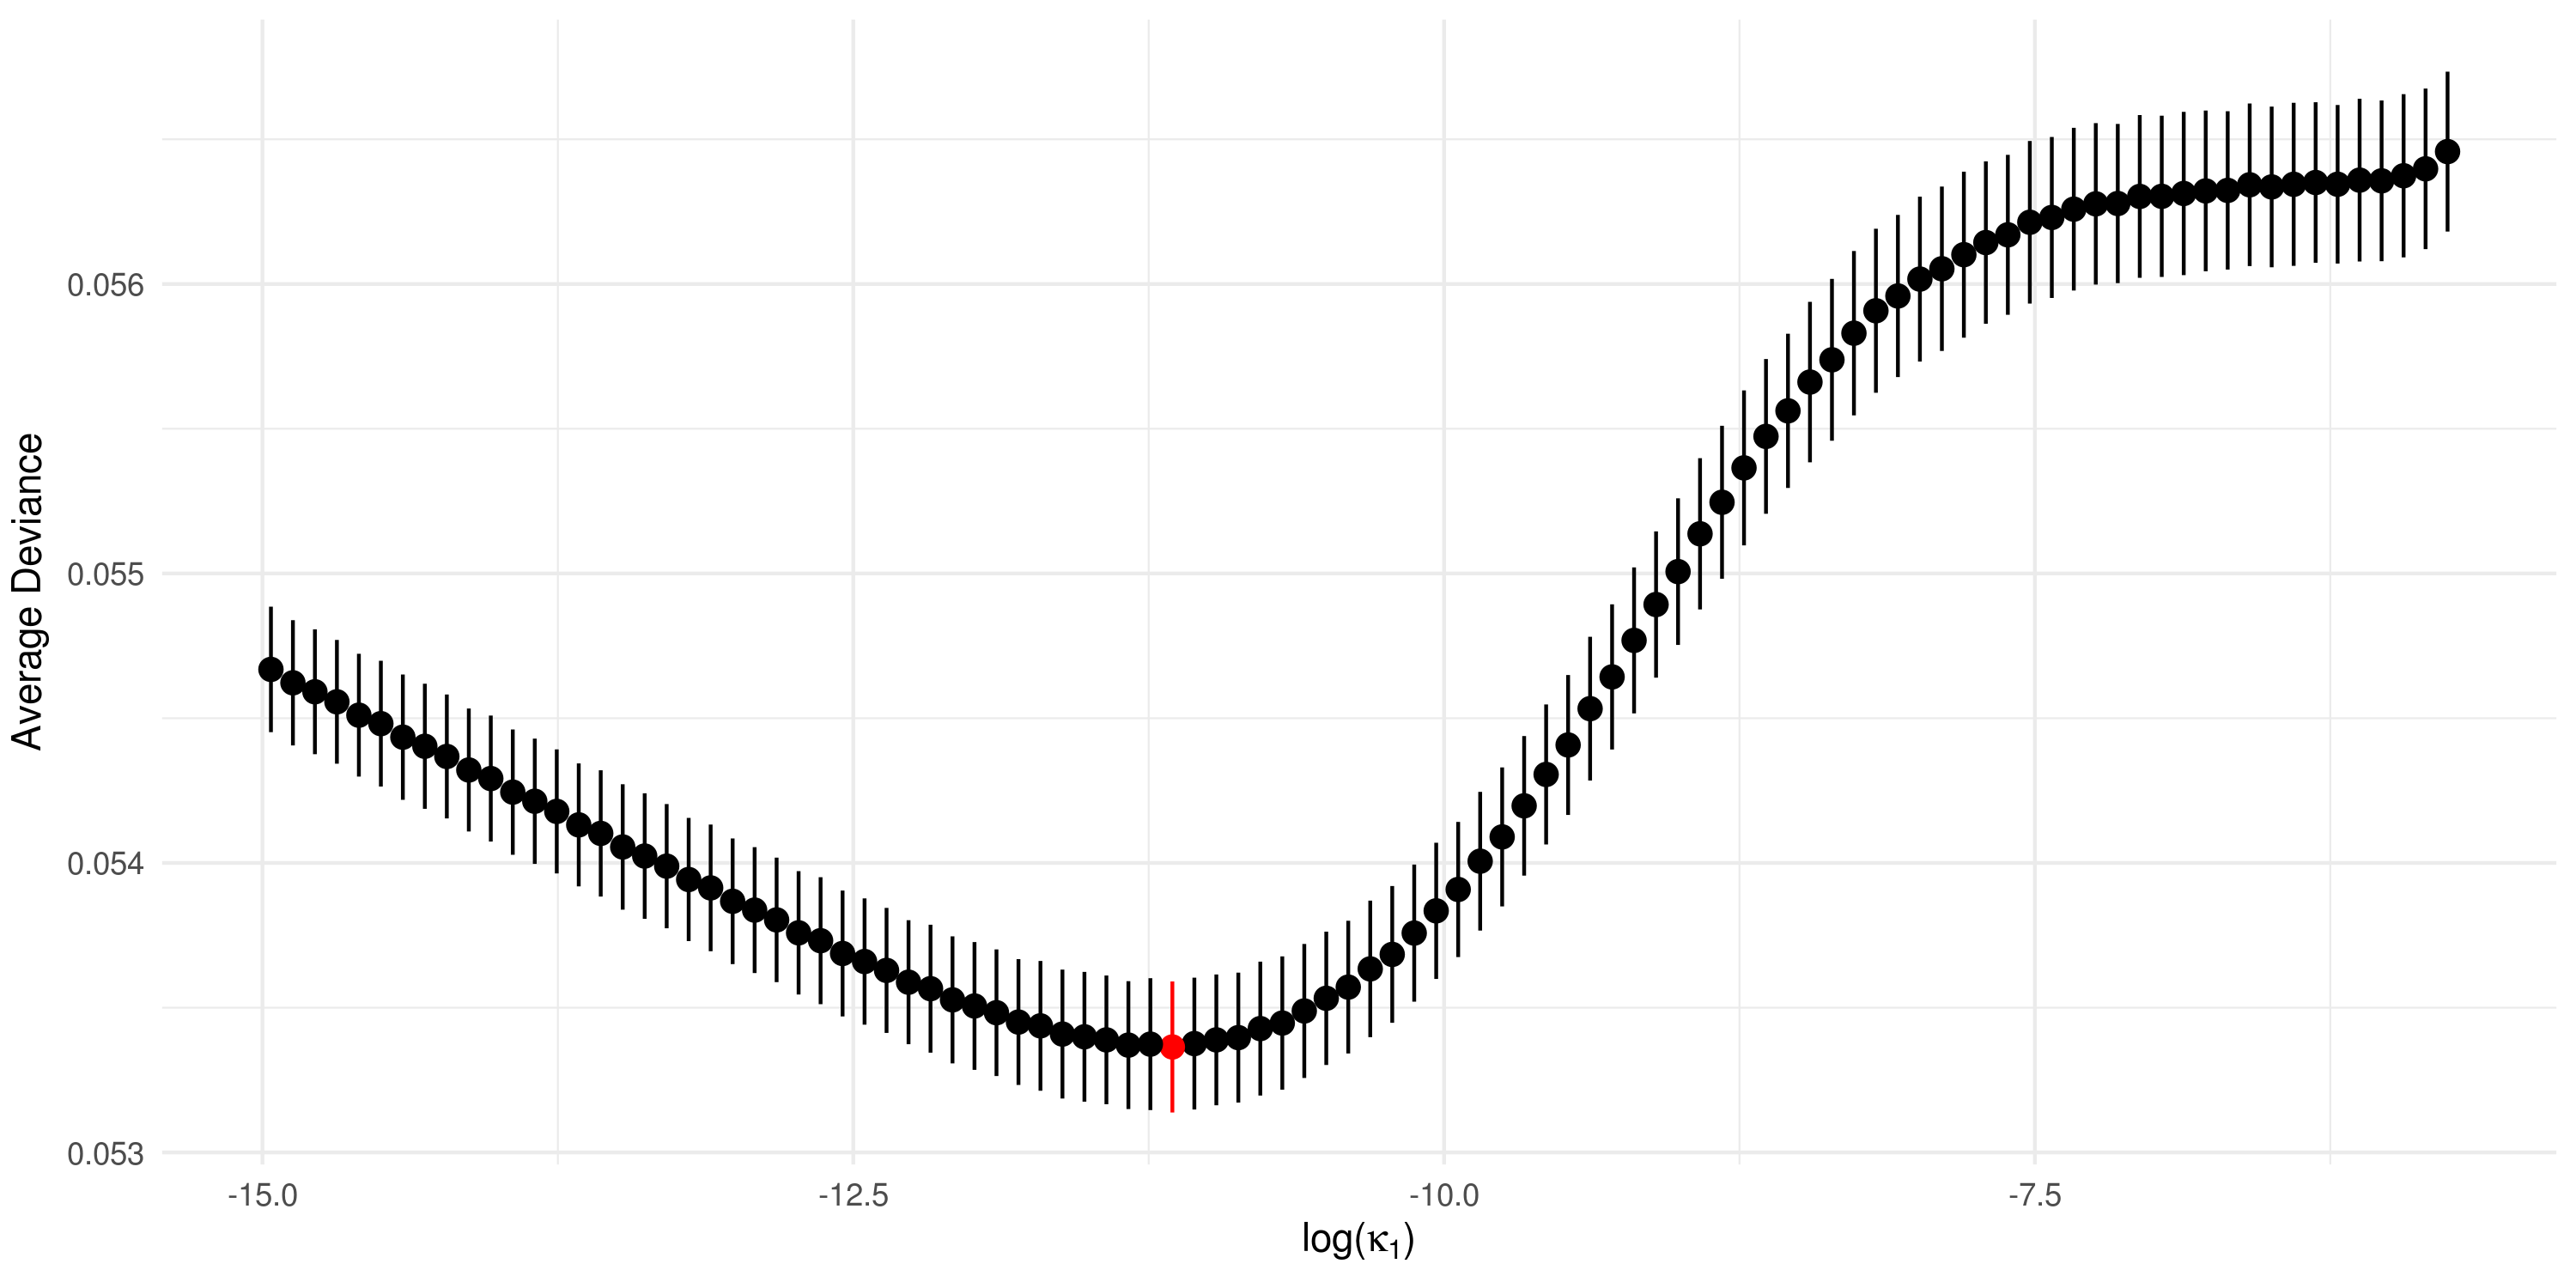
\includegraphics[width=4in]{figures/fig3.png}
\vspace*{0mm}
\caption{The average deviance (with one standard deviation) across the 10 folds in our cross-validation procedure plotted against $\log(\kappa_1)$. The minimum deviance is highlighted red.\label{fig:genmodelstats}}
\vspace*{-2mm}
\end{figure}

\begin{figure}[htbp]
\centering
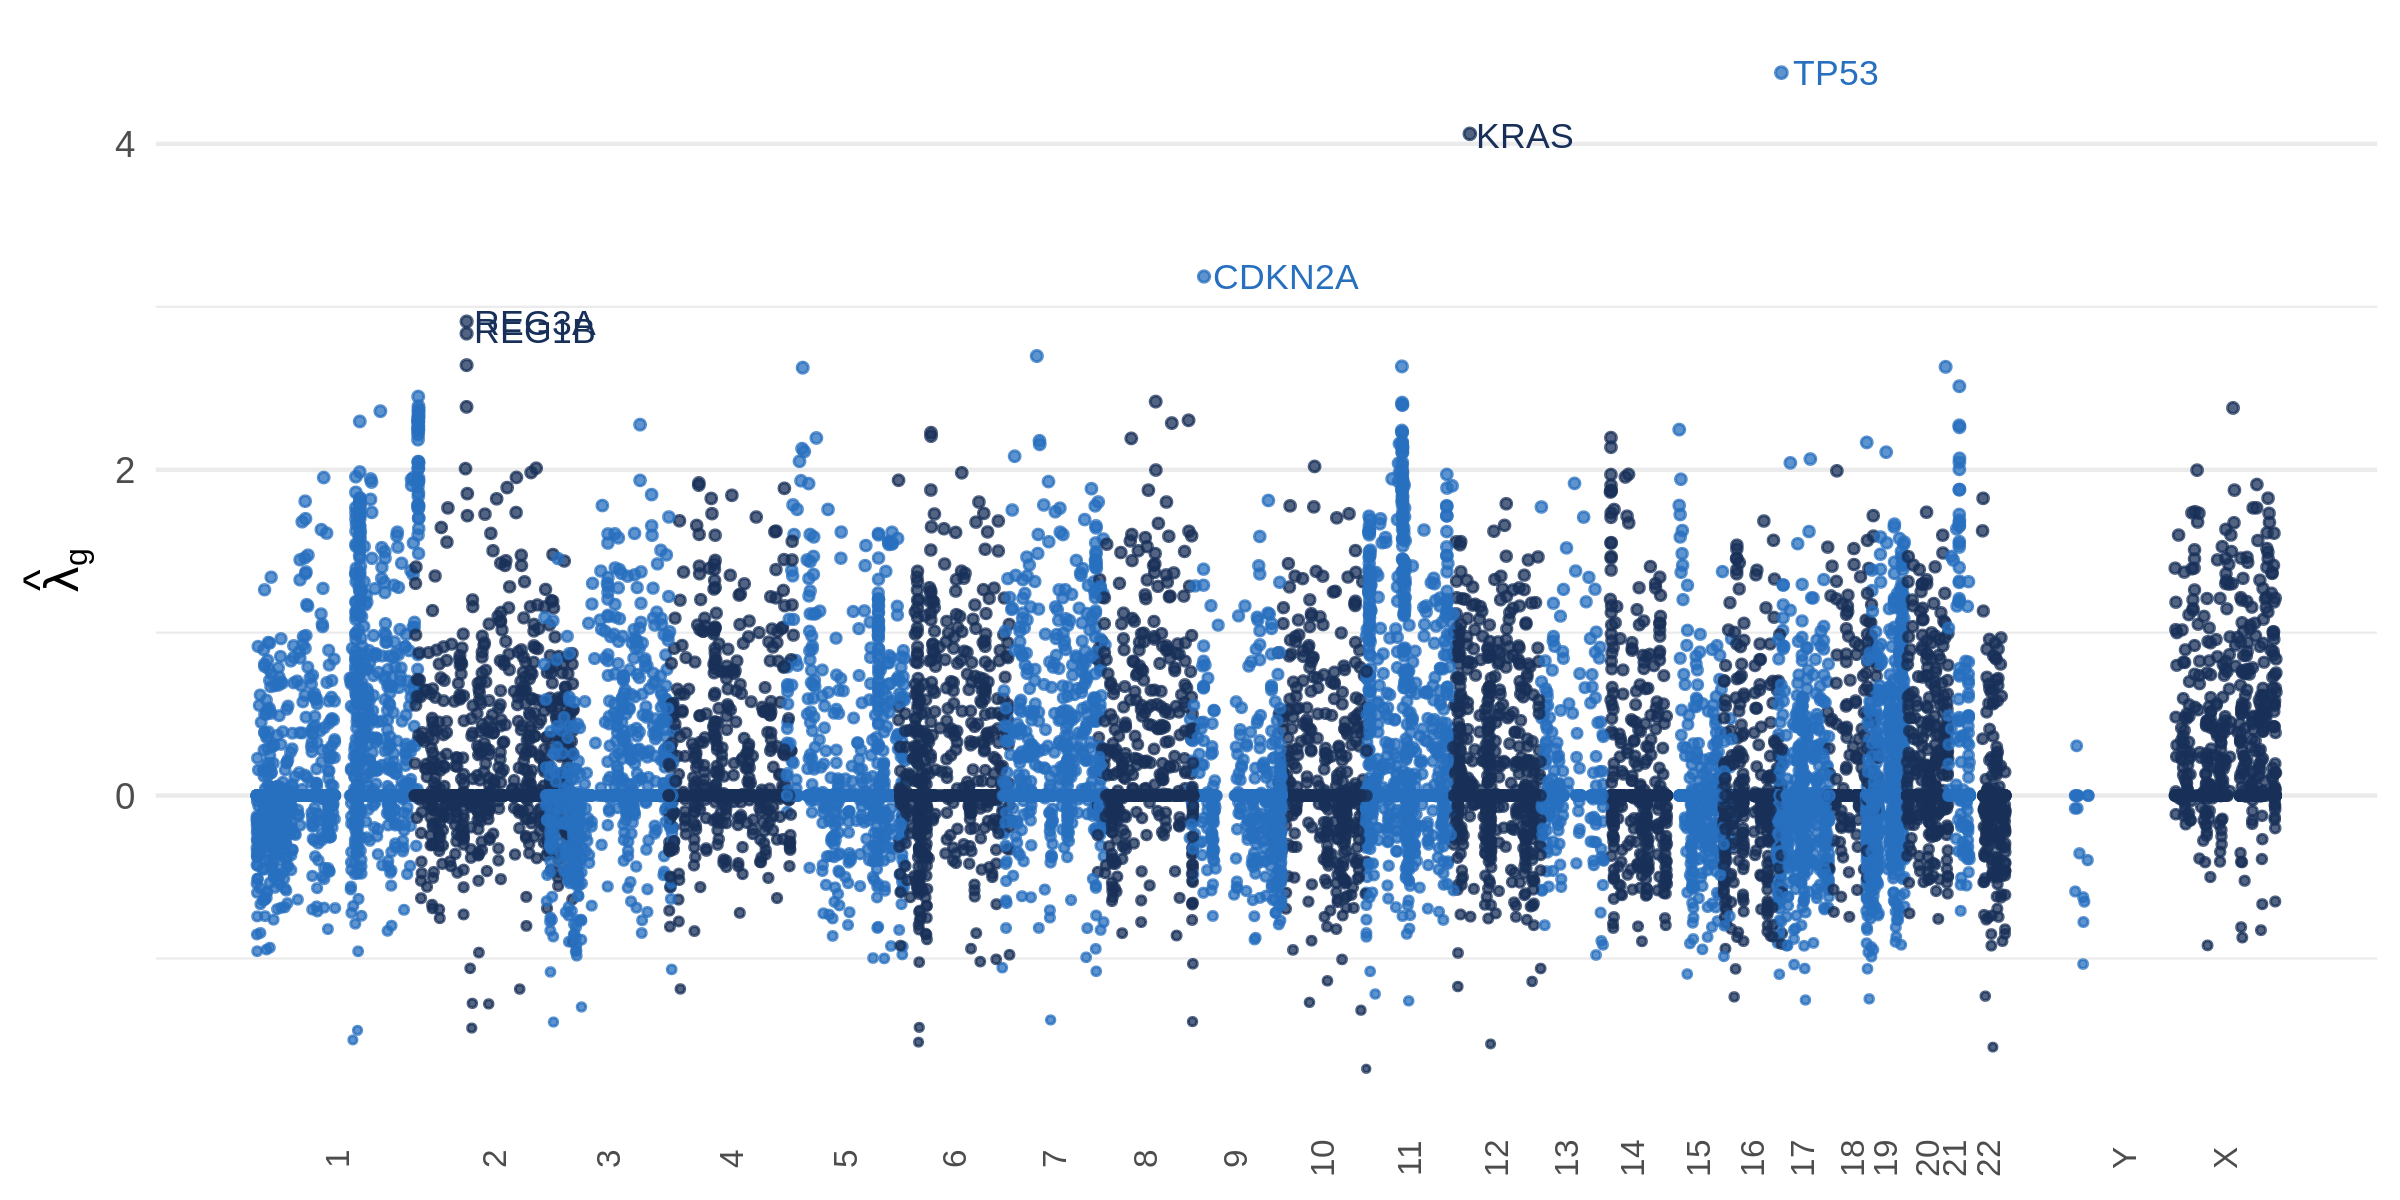
\includegraphics[width=6in]{figures/fig4.png}
\vspace*{0mm}
\caption{Manhattan plot of fitted parameters $\hat{\lambda}_g$ and their associated genes' chromosomal locations. The genes with the five largest positive parameter estimates are labelled. \label{fig:manhat_plot}}
\end{figure}

\begin{figure}[htbp]
\centering
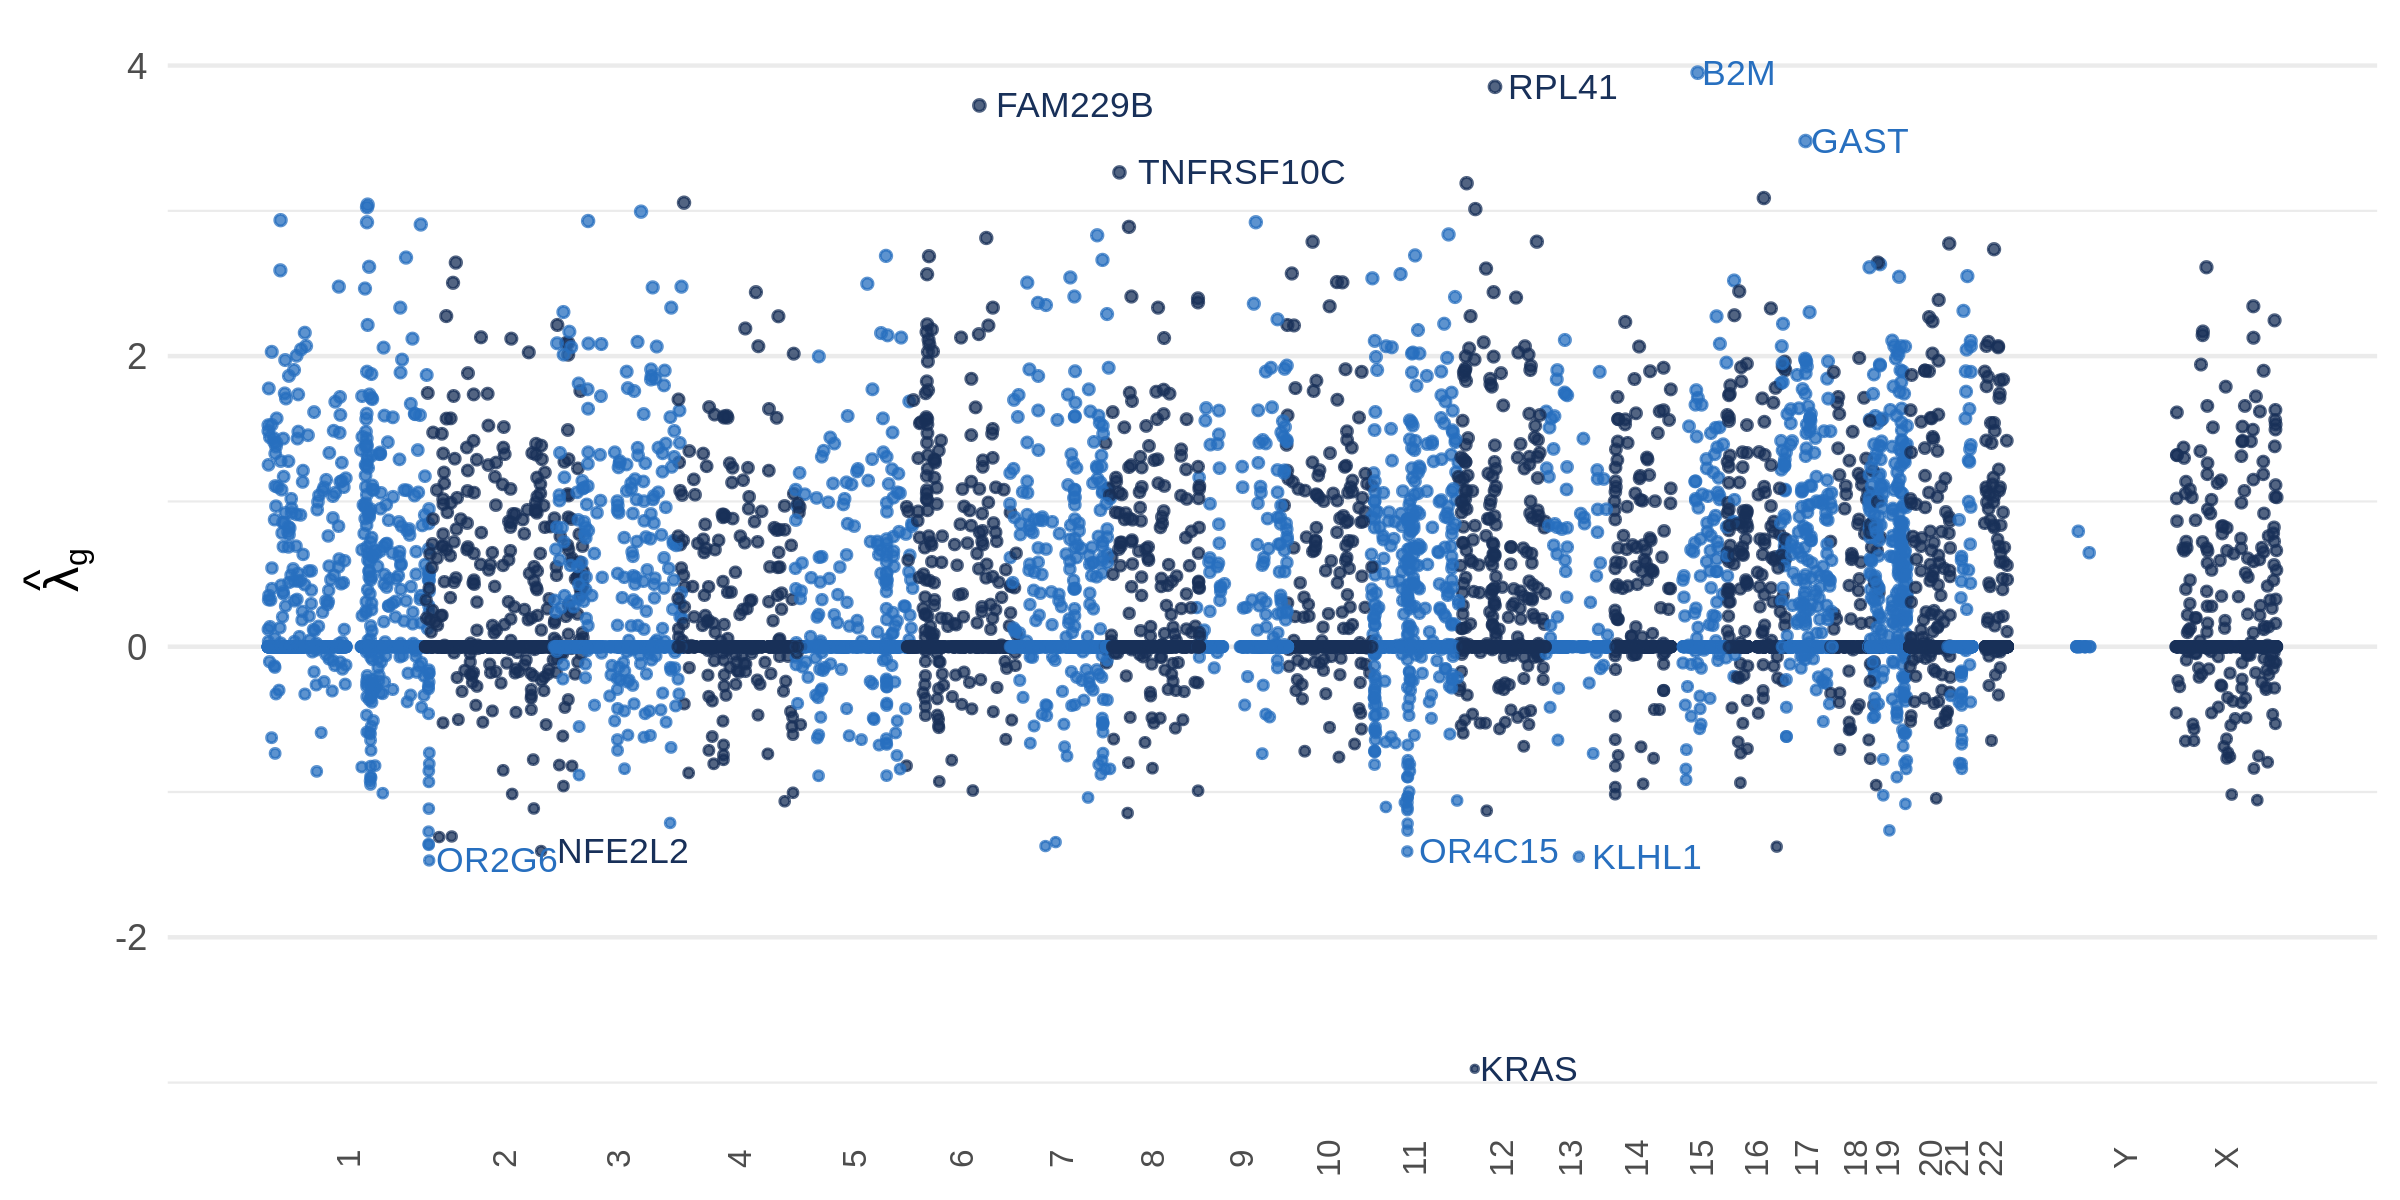
\includegraphics[width=6in]{figures/fig5.png}
\caption{Manhattan plot of fitted parameters $\hat{\eta}_{g,\text{indel}}$ and their associated genes' chromosomal locations. The five largest positive and negative genes are labelled.  \label{fig:manhat_plot_indel}}
\end{figure}
In order to provide some validation of the model formulation in \eqref{eq:loglink}, we compare our model with the following alternatives: 
%performed \jbnote{'deviance comparisons'} on our model against a range of alternatives. 
\begin{enumerate}[(i)]
\item Saturated model: each observation has an associated free parameter (i.e. $\phi_{igs} > 0$ in \eqref{eq:Poisson} is unrestricted);
\item No sample-specific effects:  $\mu_i = 0$ for all $i \in \{1,\ldots, n\}$;
\item No gene-specific effects: $\lambda_g = \eta_{gs} = 0$ for all $g \in G$ and $s\in S$; 
\item No gene/mutation type interactions: $\eta_{gs} =0$ for all $g \in G$ and $s\in S$.
\end{enumerate}

In Table~\ref{table:goodnessoffit} we present the residual deviance and the residual degrees of freedom between our model and each of the models above. First note that the decrease in deviance between our model and model (i) is very small relative to the additional degrees of freedom associated with the saturated model; this suggests that our model is more appropriate. On the other hand, when comparing our model with the alternatives in (ii)-(iv), the decrease in deviance large relative to the increase in degrees of freedom, and our model is therefore preferred.    

%Other than these restrictions we fitted each submodel in exactly the same way as described in Section \ref{sec:genmodel}. 
%The results of these comparisons are given in Table \ref{table:goodnessoffit}. We see that making any of the restrictions discussed severely inhibits the explanatory power of the generative model, even when allowing for the residual degrees of freedom in the larger model. Furthermore a saturated model does not offer nearly enough improved prediction to justify the large increase in degrees of freedom. 

%We see strong evidence that it is necessary to incorporate both sample-specific and gene-specific parameters into a model of mutation, but that a saturated model does not nearly give enough improvement in prediction to justify its vastly increased degrees of freedom. We find $p$-values indistinguishable from 0 and 1 - these should not be interpreted too strongly, as various high-dimensional and model selection effects can come to bear when quantifying such comparisons. 

%Modern methods for testing goodness-of-fit of high dimensional generalised linear models such as proposed by \citet{jankova_goodness--fit_2019} are discussed in Appendix \ref{app:goodnessoffit}, including a proposal for using such methodology to predict genes containing hotspot codons. 

\begin{table}[ht]
\begin{center}
\caption{Model comparisons on the basis of residual deviance statistics. \label{table:goodnessoffit}}
\begin{tabular}{ | c | c | c | c  | c |}
\hline
Comparison  & Residual  & Residual Degrees & dev/df & $p$-value \\
Model            & Deviance (dev)             & of Freedom (df)  &        &           \\
\hline
(i) &  $7.50 \times 10^5$  & $2.80\times 10^7$  &  $2.68 \times 10^{-2}$   &  1.00 \\
\hline
(ii)  &  $1.61 \times 10^5$  &  $8.00 \times 10^2$  &  $2.01 \times 10^2$ &  0.00\\
(iii)  &  $2.00 \times 10^5$ & $3.49 \times 10^4$  & $5.74 \times 10^0$&  0.00 \\
(iv) & $1.09 \times 10^5$ & $1.75 \times 10^4$ & $1.09 \times 10^1$ & 0.00 \\
\hline
\end{tabular}
\vspace*{-10mm}
\end{center}
\end{table}


\subsection{Predicting tumour mutation burden \label{sec:tmb}}
We now demonstrate the excellent practical performance of our procedure for estimating \acrshort{tmb}. Recall that \acrshort{tmb} is given by equation~\eqref{eq:biomarker} with $\bar{S}$ being the set of all non-synonymous mutation types. First it is shown that our method can indeed select gene panels of size specified by the practitioner and that good predictions can be made even with small panel sizes (i.e.~$\leq$ 1Mb). We then compare the performance of our proposal with state-of-the-art estimation procedures based on a number of widely used gene panels.

In order to evaluate the predictive performance of an estimator we calculate the $R^2$ score on the validation data. More precisely, given predictions of \acrshort{tmb}, $\hat{t}_1, \ldots, \hat{t}_{n_{val}}$, for the observations in the validation set with true \acrshort{tmb} scores $t_1, \ldots, t_{n_{val}}$. Let $\bar{t} := \frac{1}{n_{val}} \sum_{i=1}^{n_{val}} t_i$, and let 
    \[
    R^2 = 1- \frac{\sum_{i =1}^{n_{val}}(t_i - \hat{t}_i)^2}{\sum_{i = 1}^{n_{val}}(t_i - \bar{t})^2}. 
    \]
 While it's not the focus of our approach, other works have been interested in separating tumours into two classes (High \acrshort{tmb}, Low \acrshort{tmb}) \citep{buttner_implementing_2019, wu_designing_2019}. We therefore also report the estimated area under the precision-recall curve (\acrshort{auprc}) for a classifier based on our approach. The \acrshort{auprc} is calculated as follows: first, in line with major clinical studies \citep[see, for example,][]{hellmann_nivolumab_2018, ramalingam_abstract_2018}, the true class membership of a tumour is defined according to whether it has $t^* := 300$ or more exome mutations (approximately 10 Mut/Mb). This gives 53 (30.8\%) tumours with high \acrshort{tmb} and 119 (69.2\%) with low \acrshort{tmb} in the validation set. Now, for a cutoff $t \geq 0$, let 
 \[
 p(t) := \frac{\sum_{i=1}^{n_{val}} \mathbbm{1}_{\{\hat{t}_i \geq t, \ t_i \geq t^*\}}}{\sum_{i=1}^{n_{val}} \mathbbm{1}_{\{\hat{t}_i \geq t\}}}; \quad  r(t) := \frac{\sum_{i=1}^{n_{val}} \mathbbm{1}_{\{\hat{t}_i \geq t, \ t_i \geq t^*\}}}{\sum_{i=1}^{n_{val}} \mathbbm{1}_{\{t_i \geq t^*\}}}
 \]
 be the estimated (over the validation set) precision and recall, respectively, of a classifier that assigns a tumour to the High \acrshort{tmb} class if its estimated \acrshort{tmb} is greater than or equal to $t$.  The precision-recall curve is $\{(r(t),p(t)): t \in [0, \infty)\}$. Note that a perfect classifier achieves a \acrshort{auprc} of 1, whereas a random guess in this case would have an average \acrshort{auprc} of 0.308 (the prevalence of the High \acrshort{tmb} class).
% although standardisation of TMB thresholds is an open endeavour \citep{chang_p086_2018, stenzinger_tumor_2019}. 
%$R^2$ score and Area Under Precision/Recall Curve (\acrshort{auprc}). 

%For predictions $\hat{t}_i \ (i \in \{1,\ldots, n_{val}\})$, where $n_{val}$ is the number of validation samples, of true TMB scores $t_i$ with mean $\bar{t}_i$, we take  

\begin{figure}[ht]
\centering
\vspace{-5mm}
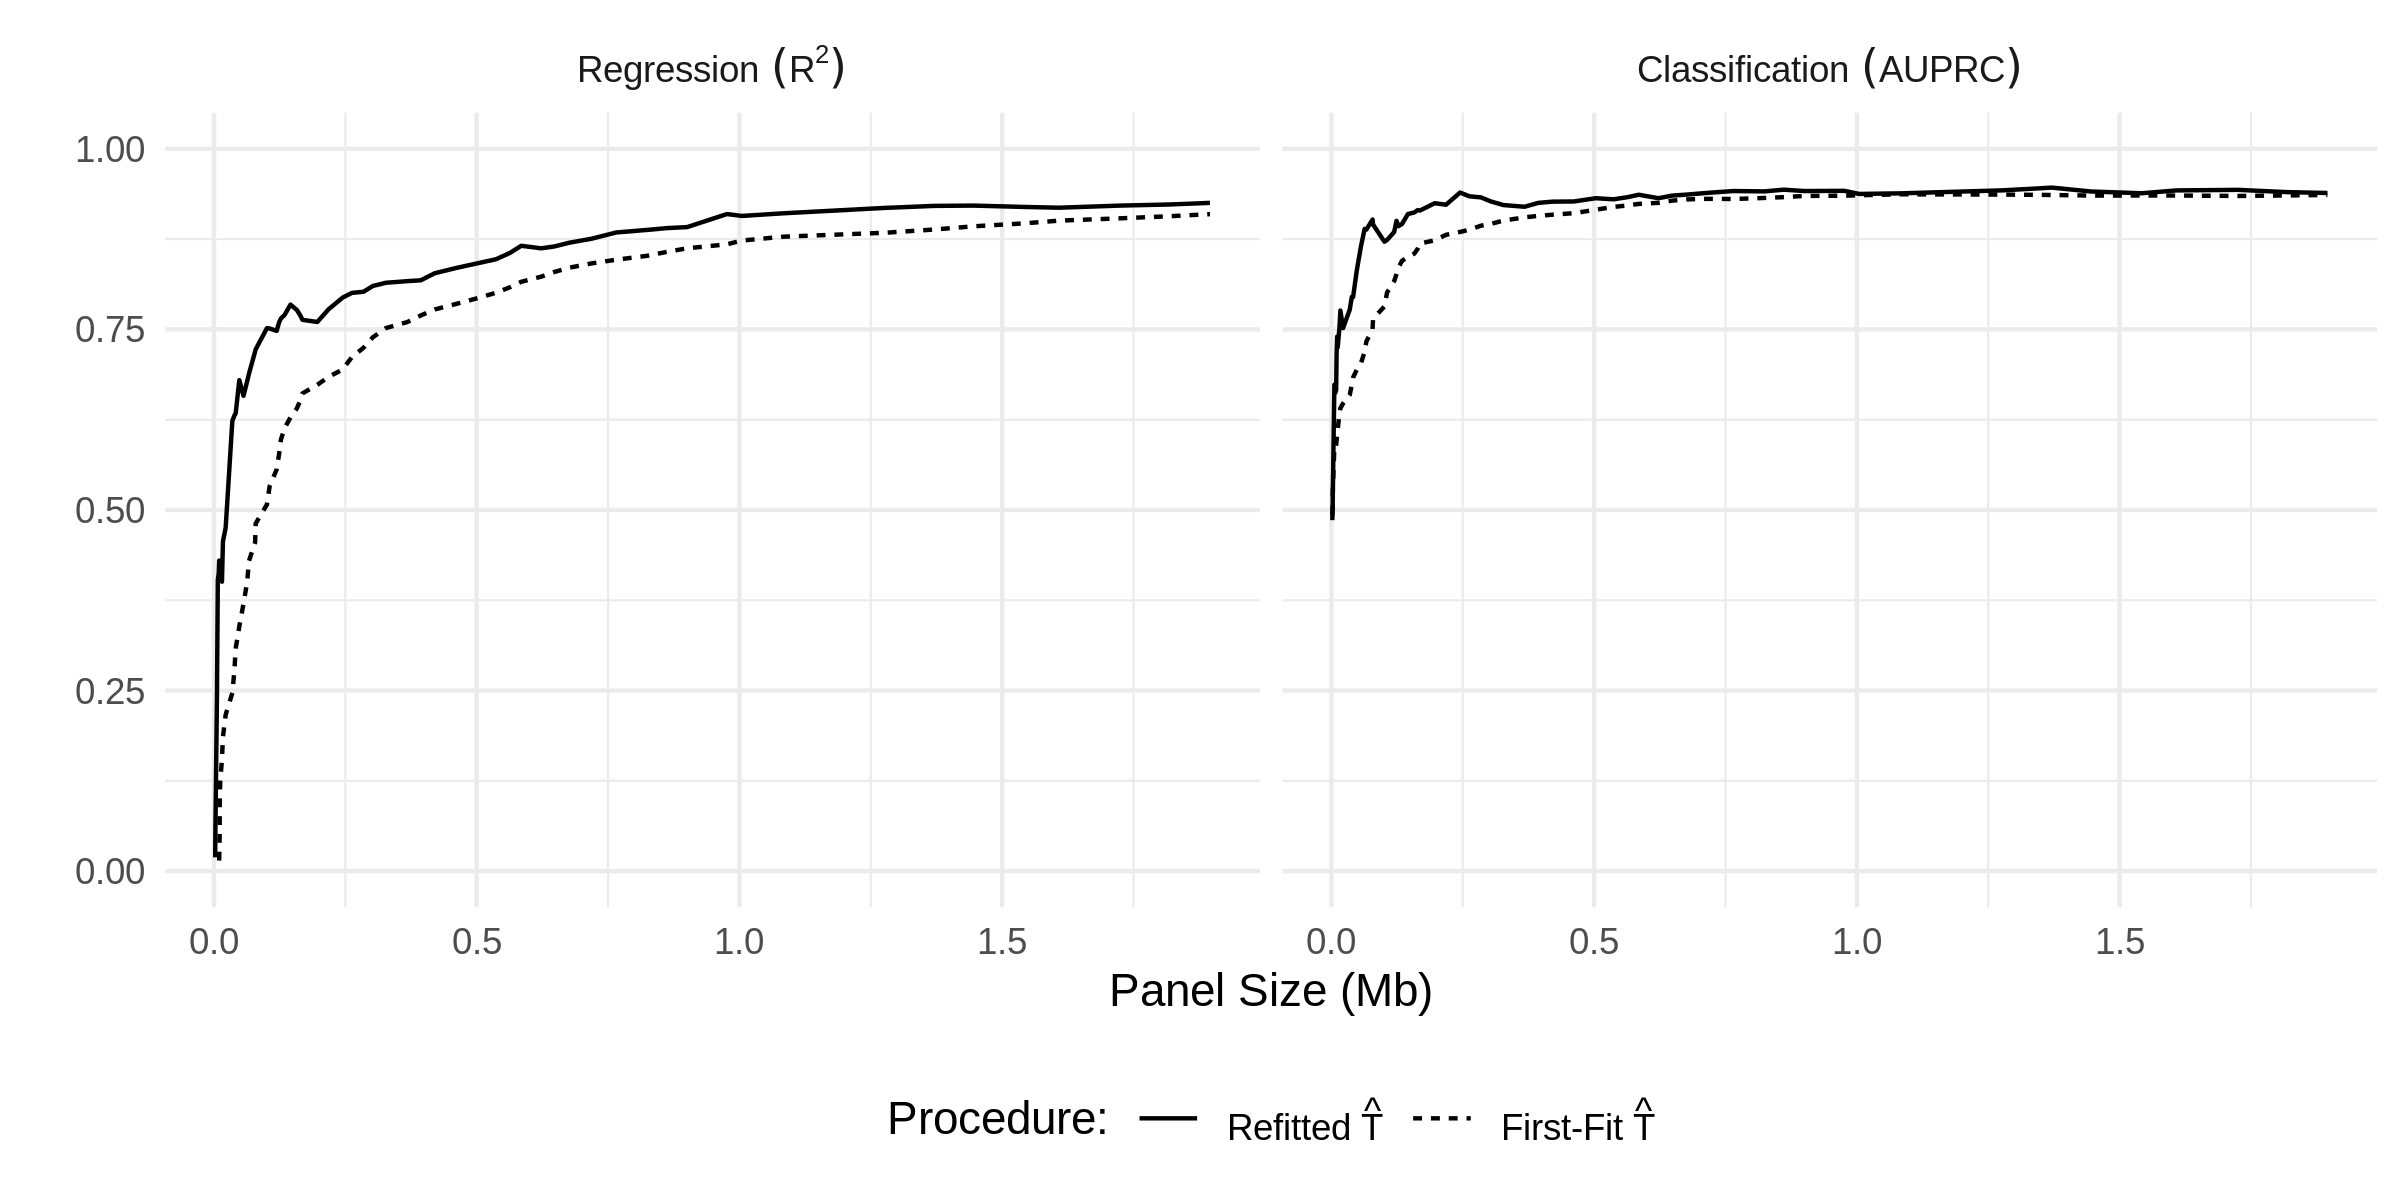
\includegraphics[width=6in]{fig6.png}
\vspace*{-5mm}
\caption{Performance of our first-fit and refitted estimators of \acrshort{tmb} as the selected panel size varies. \textbf{Left}: $R^2$, \textbf{Right}: \acrshort{auprc}. \label{fig:EstimatorPerformance}}
\vspace*{-2mm}
\end{figure}

To estimate \acrshort{tmb} we apply our procedure in Section~\ref{sec:linearestimator} with $\bar{S} = S$, where the model parameters are estimated as described in Section~\ref{sec:genmodelfit}. In Figure~\ref{fig:EstimatorPerformance}, we present the $R^2$ and \acrshort{auprc} for the first-fit and refitted estimators (see~\eqref{eq:wfirstfit} and~\eqref{eq:wrefit}, respectively) as the selected panel size varies from 0Mb to 2Mb in length. We see that we obtain a more accurate prediction of \acrshort{tmb}, both in terms of regression and classification, as the panel size increases, and that good estimation is possible even with very small panels (as low as 0.25Mb). %For panels less than length 0.25Mb, estimation of \acrshort{tmb} is challenging. 
Finally, as expected, the refitted estimator slightly outperforms the first-fit estimator. 

%We see elevated performance in our refitted estimator compared to the first-fit, and a sharp increase in predictive performance up to panel size around 0.25Mb, and then stably increasing performance for larger panel sizes. We see a similar trend with an even sharper corner when it comes to classification performance, as shown in Figure~\ref{fig:TvLvRF_class}.


% \begin{figure}[htbp]
% \centering
% 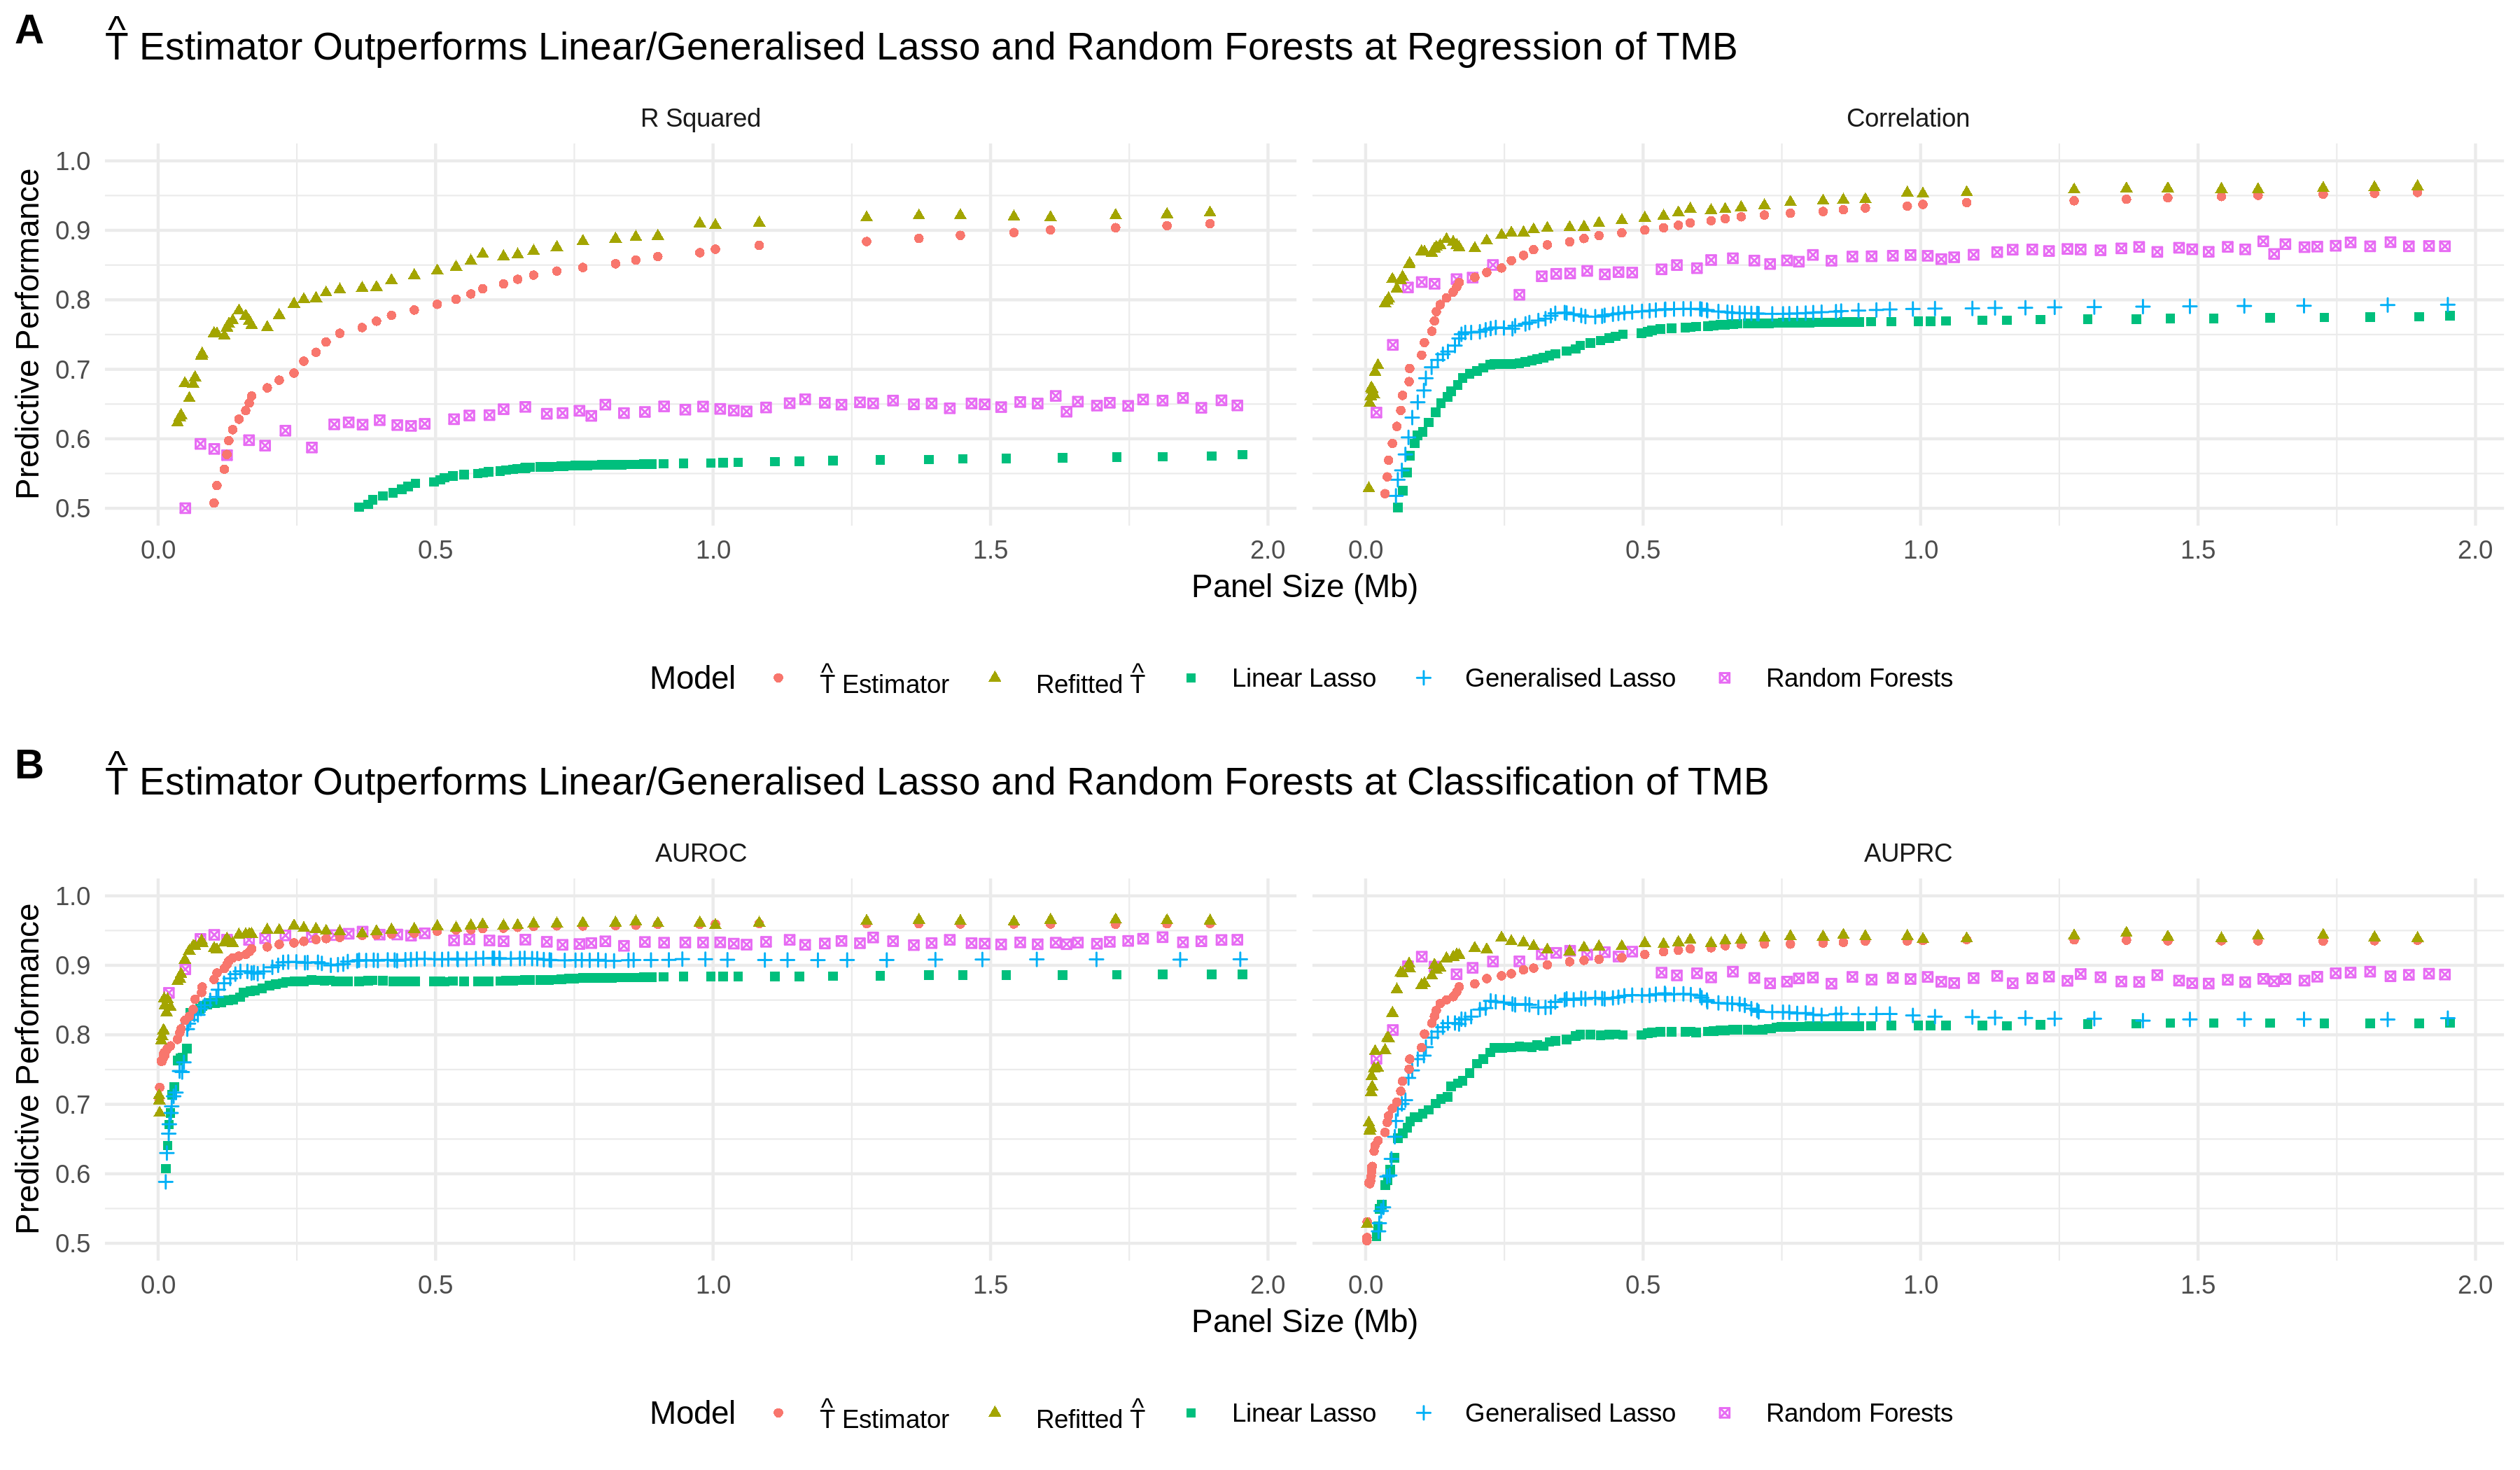
\includegraphics[width=6in]{ComparisonWithLassos.png}
% \caption{\jbnote{Get rid of correlation. Separate into three plots (second two may well disappear}\textbf{A}: Performance of regression to predict \acrshort{tmb} at different panel sizes, utilising a range of panel selection/prediction techniques (linear/generalised lasso and random forests). Regression metrics $R^2$ and correlation are shown on our validation dataset. \textbf{B}: The same comparisons, this time for classification, using area under receiver-operator characteristic and precision-recall curves as predictive metrics. \label{fig:TvLvPwithCRP}}
% \end{figure}

We now compare our method with state-of-the-art estimators applied to commonly used gene panels. The four next generation sequencing panels, Foundation~One \citep{frampton_development_2013}, MSK-IMPACT \citep{cheng_memorial_2015}, TST-170 \citep{heydt_evaluation_2018} and TSO-500 \citep{pestinger_use_2020}, are chosen for their relevance to \acrshort{tmb}. For each panel $P \subseteq G$, we use four different methods to predict \acrshort{tmb}:
\begin{enumerate}[(i)]
 \item Our refitted estimator applied to the panel $P$: we estimate \acrshort{tmb} using $T(\hat{w}_P)$, where $\hat{w}_P \in \argmin_{w \in W_P} \{f(w)\}$. 
 \item \acrshort{ectmb}: the procedure proposed by \citet{yao_ectmb_2020}.
%  \item A ridge regression model, learned on the training dataset and on the genes in the panel, and optimised by cross-validation.
 \item A count estimator: we estimate \acrshort{tmb} with $\frac{\ell_G}{\ell_P} \sum_{g \in P} \sum_{s \in S}M_{0gs}$, i.e. simply rescaling the mutation burden in the genes of $P$. 
 \item A linear model: we estimate \acrshort{tmb} with ordinary linear regression of \acrshort{tmb} against $\{M_{0gs}: g \in P, s \in S\}$.
\end{enumerate}
We include our refitted estimator applied to the panel $P$ in order to demonstrate the utility of our approach, even with a prespecified panel. The second approach is a recent method, based on a negative binomial model. The third and fourth are simple and standard practical procedures for inferring \acrshort{tmb} from targeted gene panels. 


\begin{figure}[htbp]
\centering
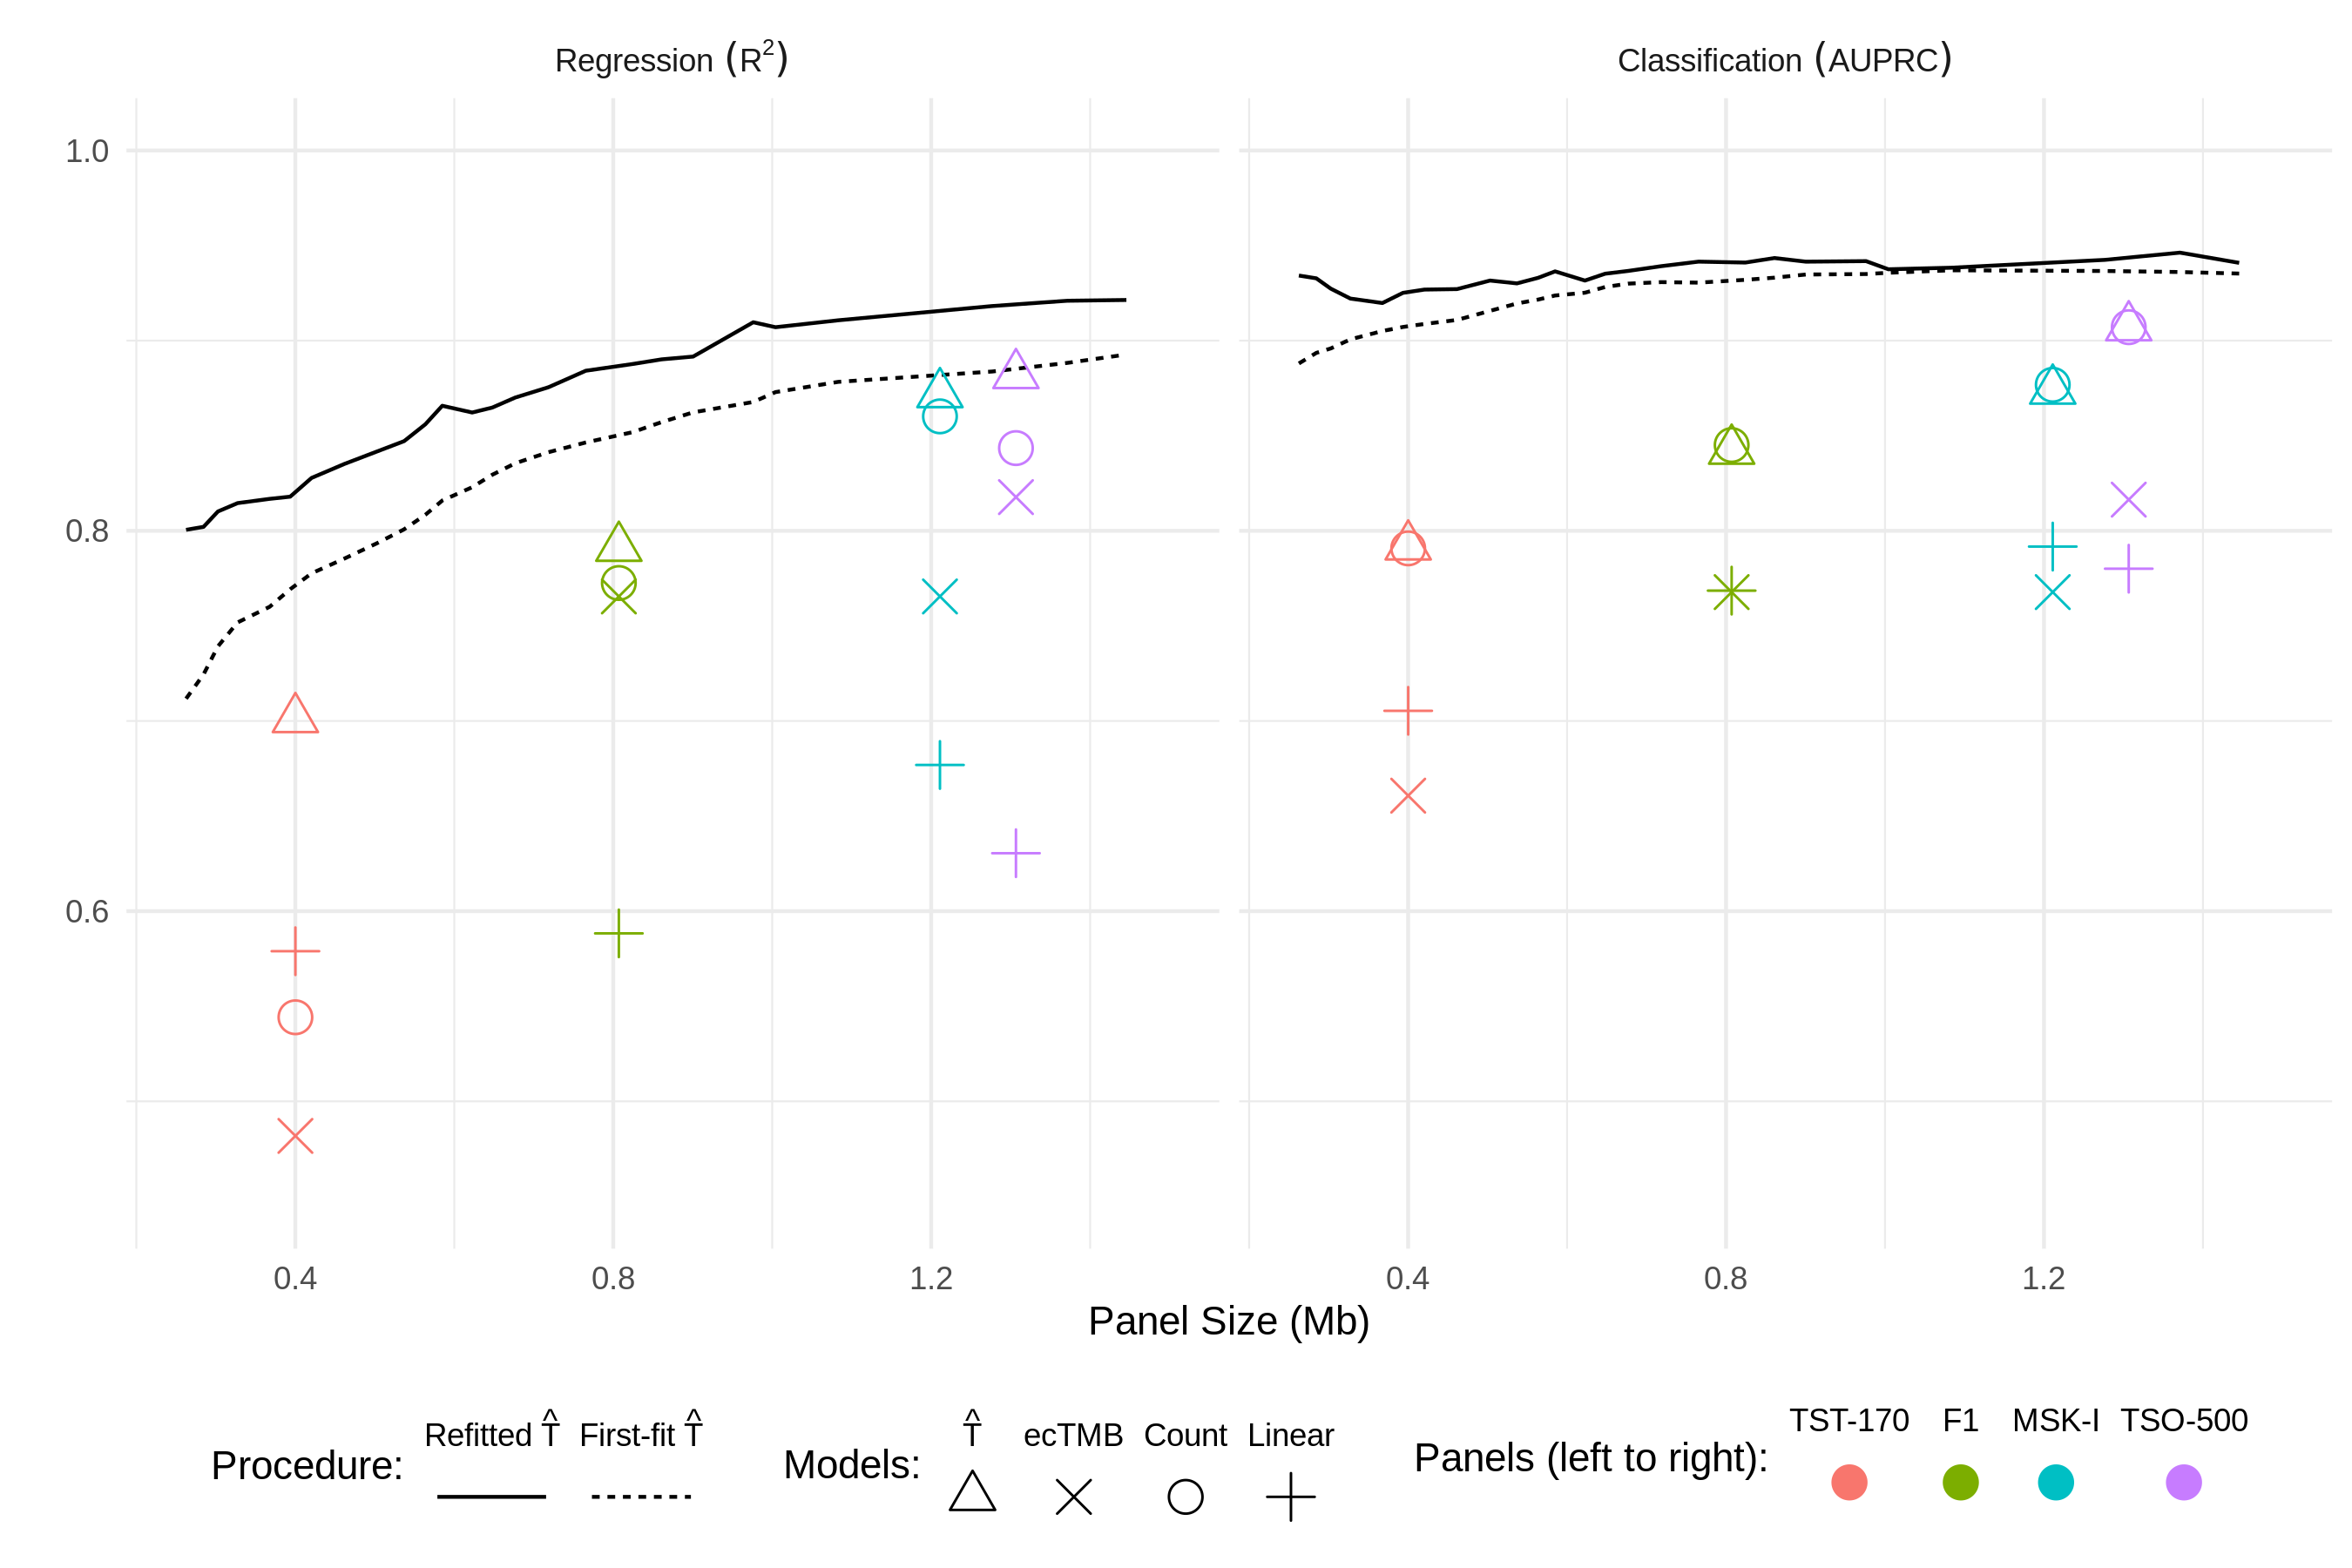
\includegraphics[width=6in]{fig7.png}
\vspace*{-5mm}
\caption{The performance of our \acrshort{tmb} estimator in comparison to existing approaches. \textbf{Left}: $R^2$, \textbf{Right}: \acrshort{auprc}. \label{fig:commercial_comparison}}
\vspace*{-2mm}
\end{figure}

We present results of these comparisons in  Figure~\ref{fig:commercial_comparison}. For each of the four panels considered here, we see that our refitted estimator applied to the panel outperforms all existing approaches in terms of regression performance, demonstrating that making predictions based on our generative model has tangible benefit. Furthermore, we see that by first selecting a panel based on the data, we are able to improve predictive accuracy even further. For instance, in comparison to predictions based on the Foundation 1 panel, our procedure with a selected panel of the same size achieves an $R^2$ of 0.88. The best available existing method based on the panel, in this case the count estimator, has an $R^2$ of 0.77. Similar results are seen for all panels included here.   In terms of classification performance, we see that good predictions based on given panels are possible using the count estimator and our refitted estimator applied to the panel. However, we see that by selecting a panel our approach is more accurate. In particular, even with the smallest panel size presented in Figure~\ref{fig:commercial_comparison}, our method is competitive with those based on the large panels.  

\begin{figure}[htbp]
\centering
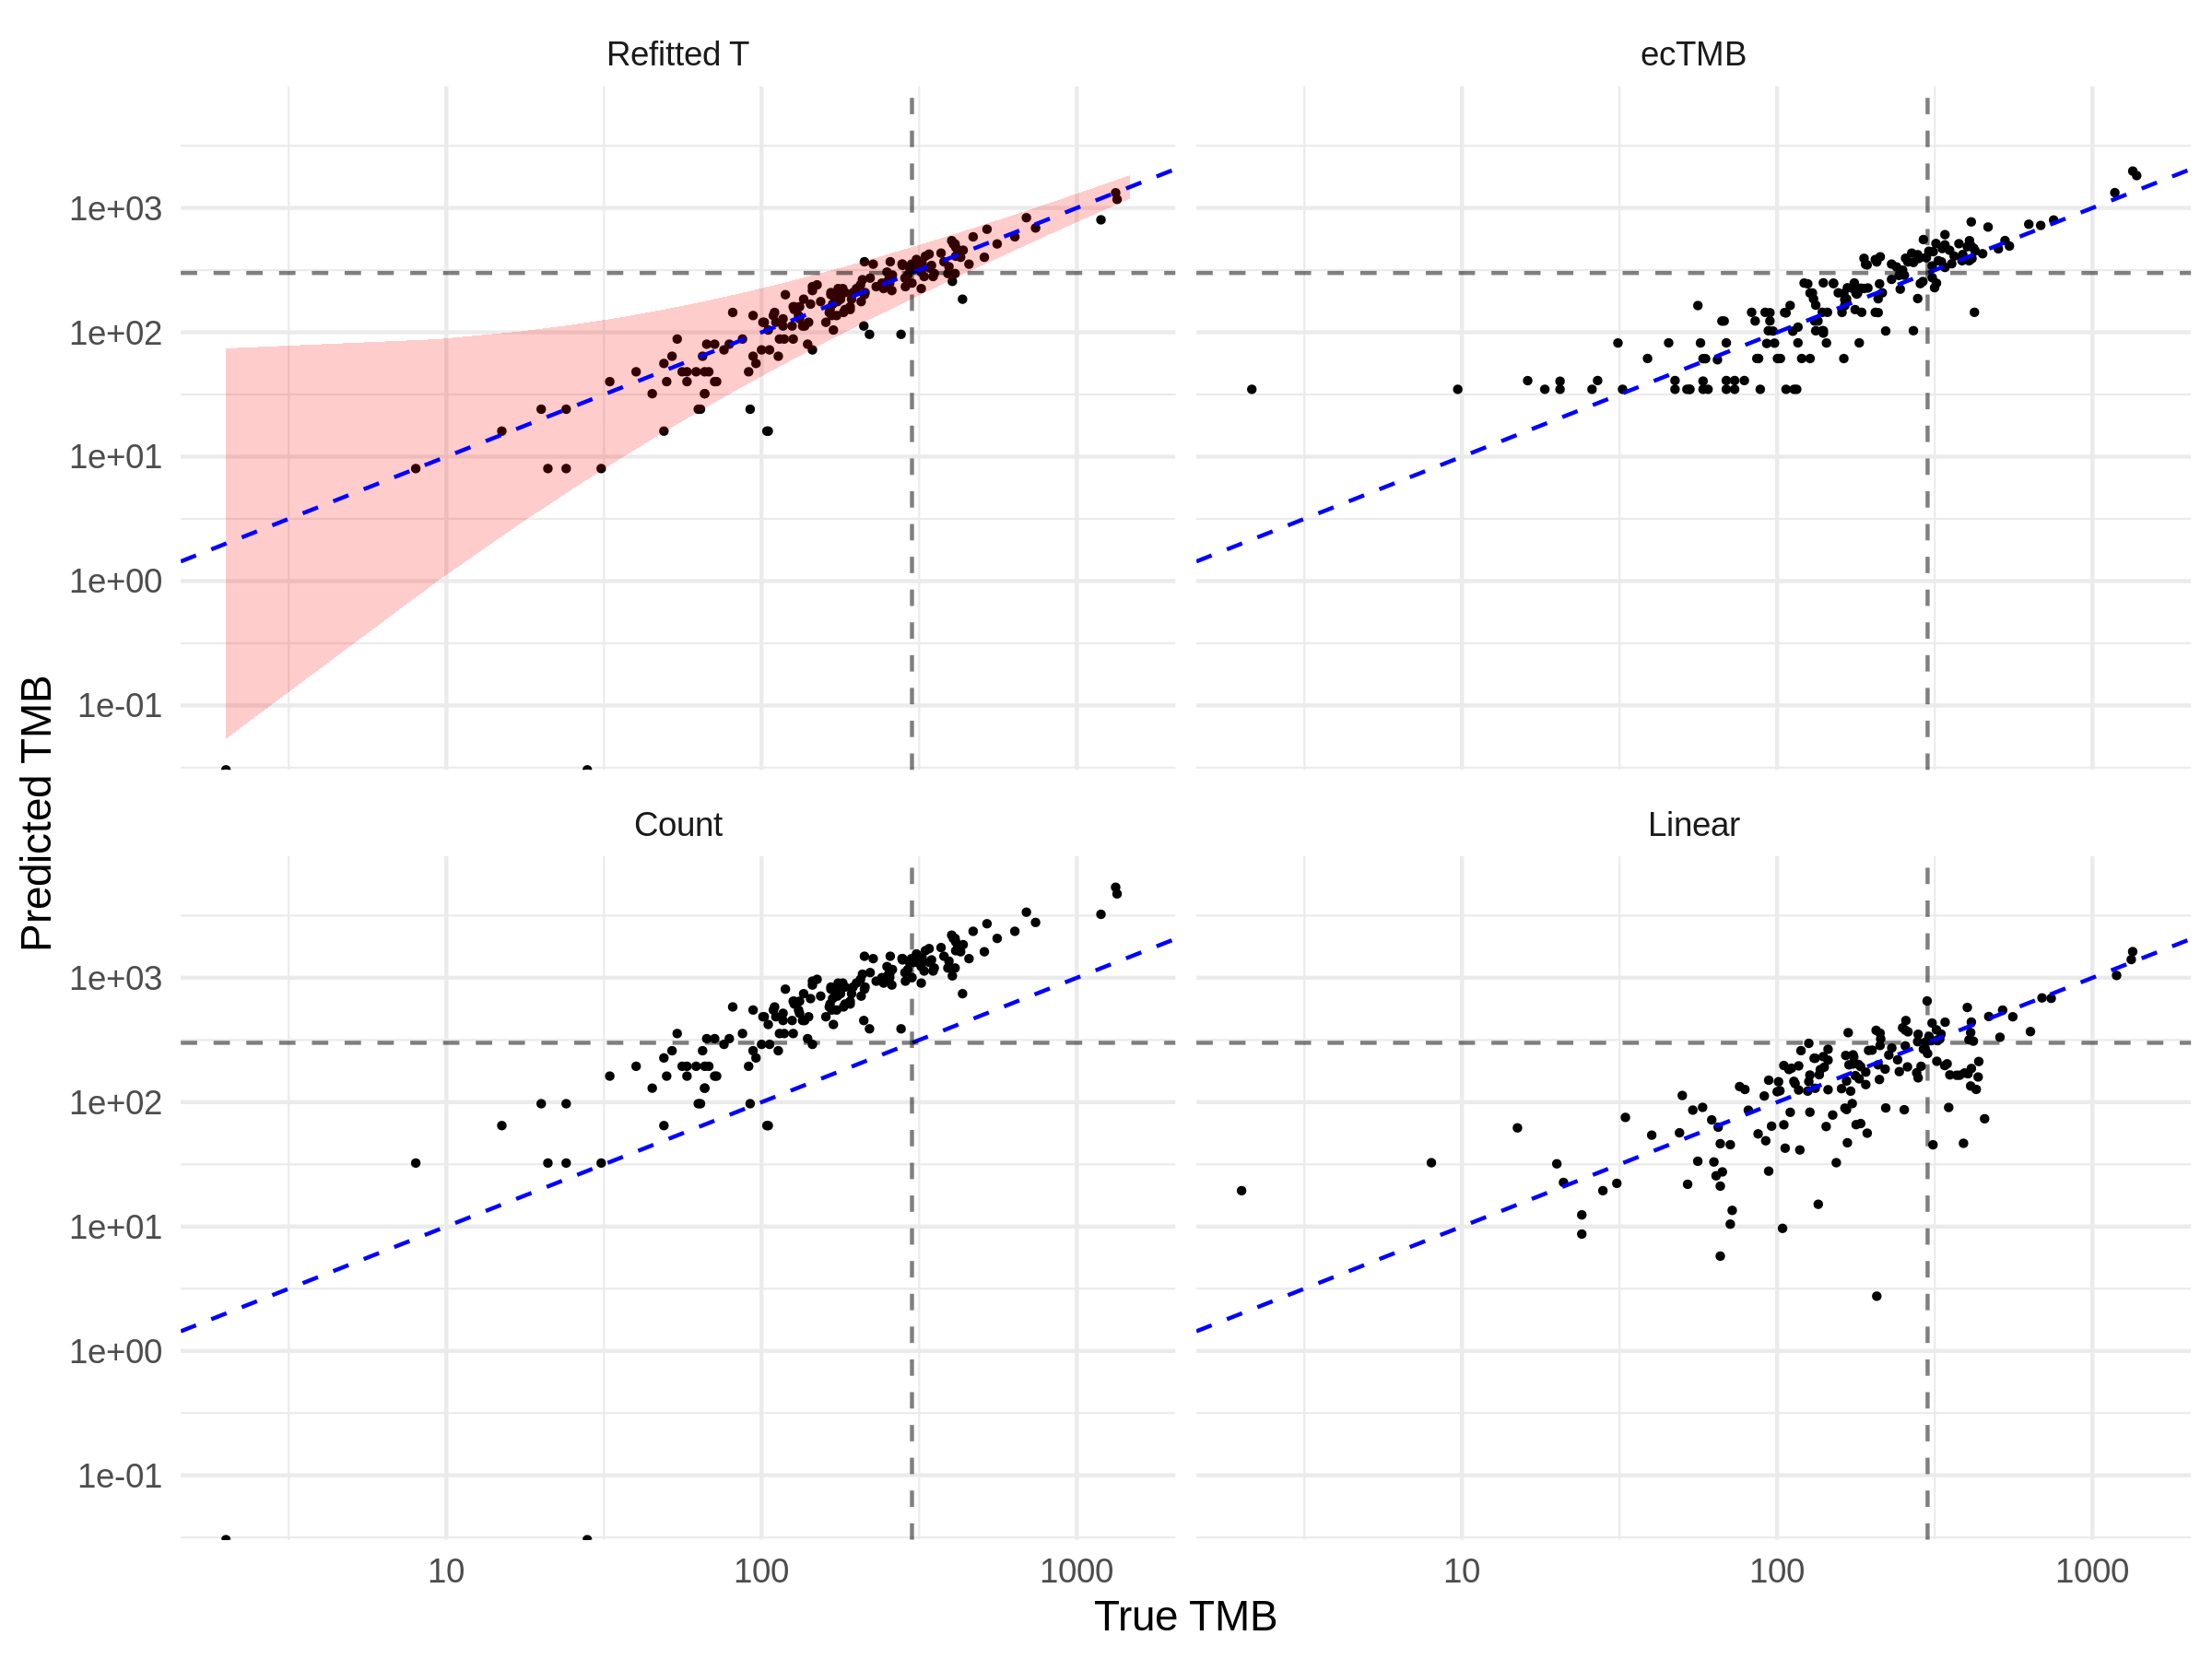
\includegraphics[width=6in]{fig8.png}
\vspace*{-5mm}
\caption{Prediction of TMB on the test dataset. Dashed blue (diagonal) line represents perfect prediction, and the black dashed lines indicate true and predicted TMB values of 300. %Red shaded area delineates region for which 90\% prediction intervals contain truth.
\label{fig:OneMBPredictions}}
\vspace*{-2mm}
\end{figure} 

Finally in this section we demonstrate the practical performance of our method using the test set, which until this point has been reserved. Based on the validation results above, we take the panel of size ~1Mb selected by our procedure and use our refitted estimator on that panel to predict \acrshort{tmb} for the samples in the test set. For comparison, we also present predictions from \acrshort{ectmb}, count-based and linear regression estimators applied to the same panel. In Figure~\ref{fig:OneMBPredictions} we see that our procedure performs very well; we obtain an $R^2$ value (on the test data) 0.89.  The other methods perform less well, with $R^2$ values of 0.72 (\acrshort{ectmb}), -19.2 (count) and 0.67 (linear). The count estimator here gives predictions which are reasonably well correlated to the true values of \acrshort{tmb} but are positively biased. This is as expected, since our selection procedure tends to favour genes with higher overall mutation rates. 
We also include a red shaded region comprising all points for which heuristic 90\% prediction intervals (as described in Section~\ref{sec:practicalconsiderations}) include the true value. We find in this case that 93.0\% of the observations in the test set fall within this region, and we therefore have valid empirical coverage.

% We see that, as expected, the count-based estimator ($R^2=-19.2$) drastically overestimates TMB, while linear regression suffers from overfitting ($R^2 = 0.67$). Estimates from the ecTMB procedure do fairly well ($R^2 = 0.72$) aside from for samples with low true TMB. 



%We see, perhaps surprisingly, that for the commercial panels ridge regression models in general performed the most poorly, despite having access within their parameter space to both of the other models. This  emphasises the issues that linear models constructed without proper justification face from overfitting, even when regularisation is introduced. We see in general that in general the density and $\hat{T}$ estimators perform similarly when measured by \acrshort{auprc}. No commercial panel achieves performance in either metric that exceeds that of a $\hat{T}$-selected panel of the same size, and particularly for classification $\hat{T}$-selected panels of far smaller size seem to produce results comparable to those of the predefined panels. We see this as a positive sign that our method has utility both for selecting \acrshort{tmb} predictive panels, and for improving the predictions of preselected panels.



% \begin{figure}[htbp]
% \centering
% 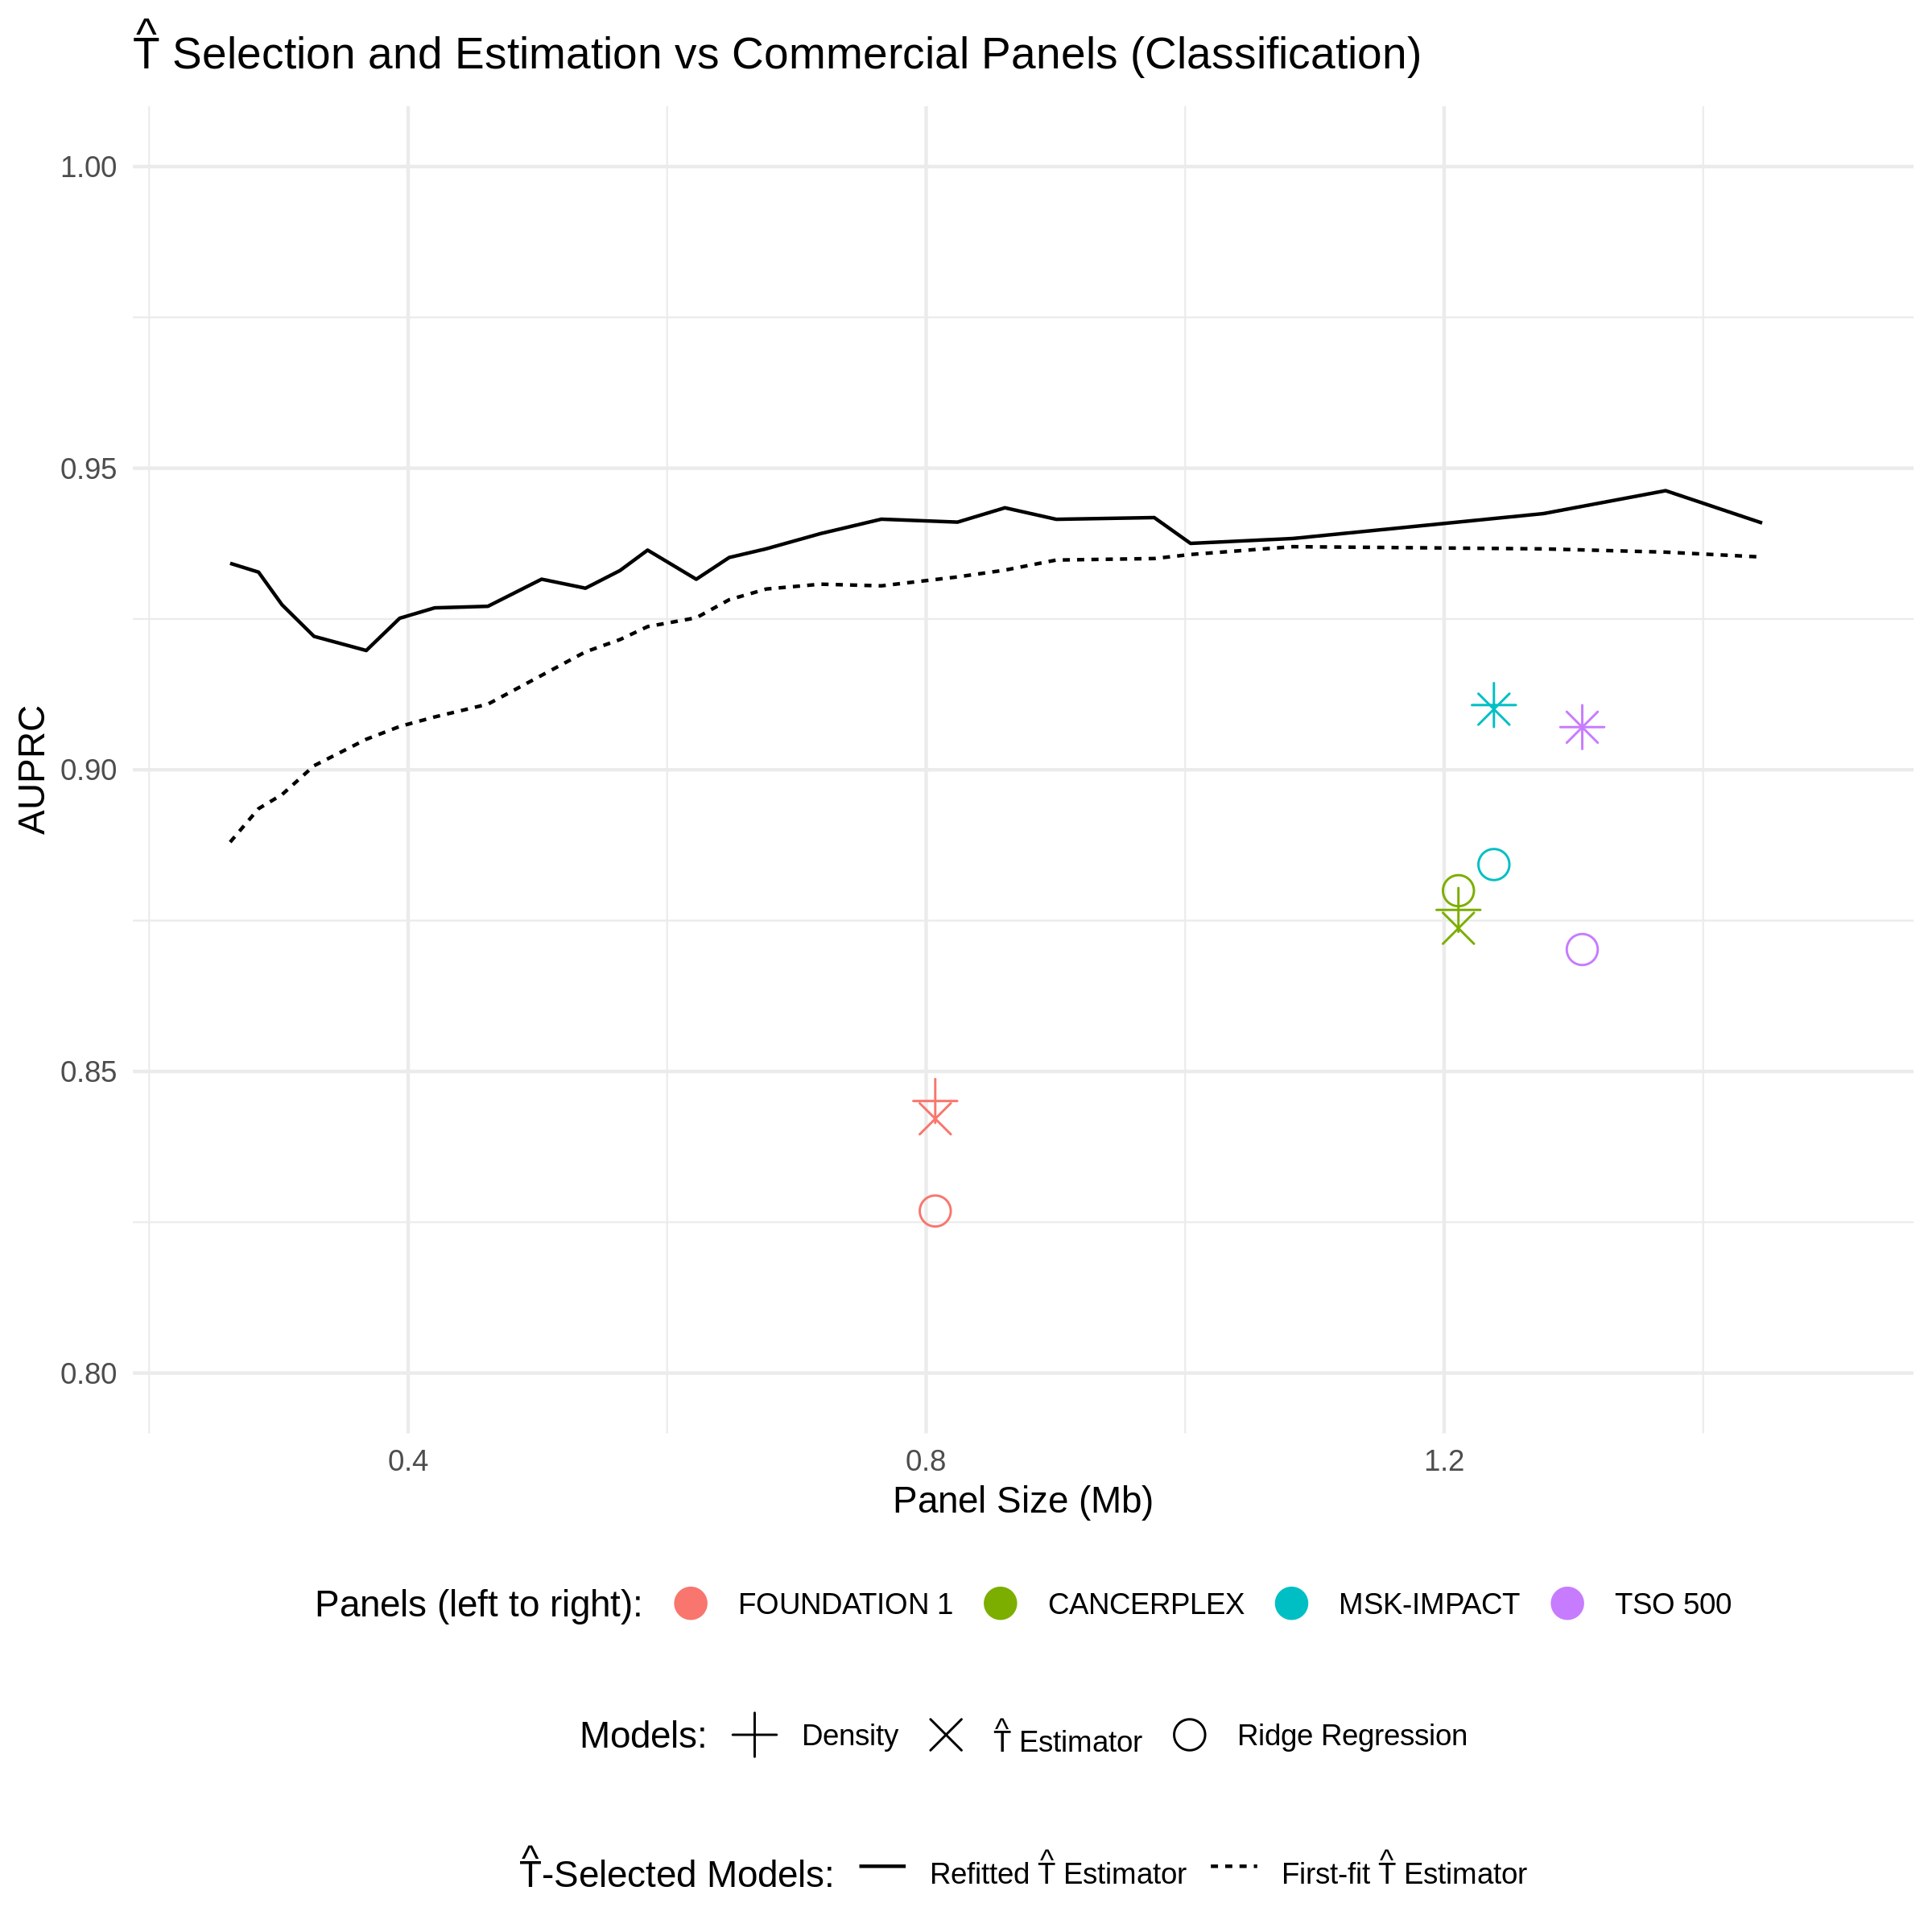
\includegraphics[width=4in]{commercial_classification.png}
% \caption{\jbnote{cut off at 0.8, move legend to caption?}\label{fig:commercial_classification}}
% \end{figure}

% % \begin{figure}
% % \centering
% % 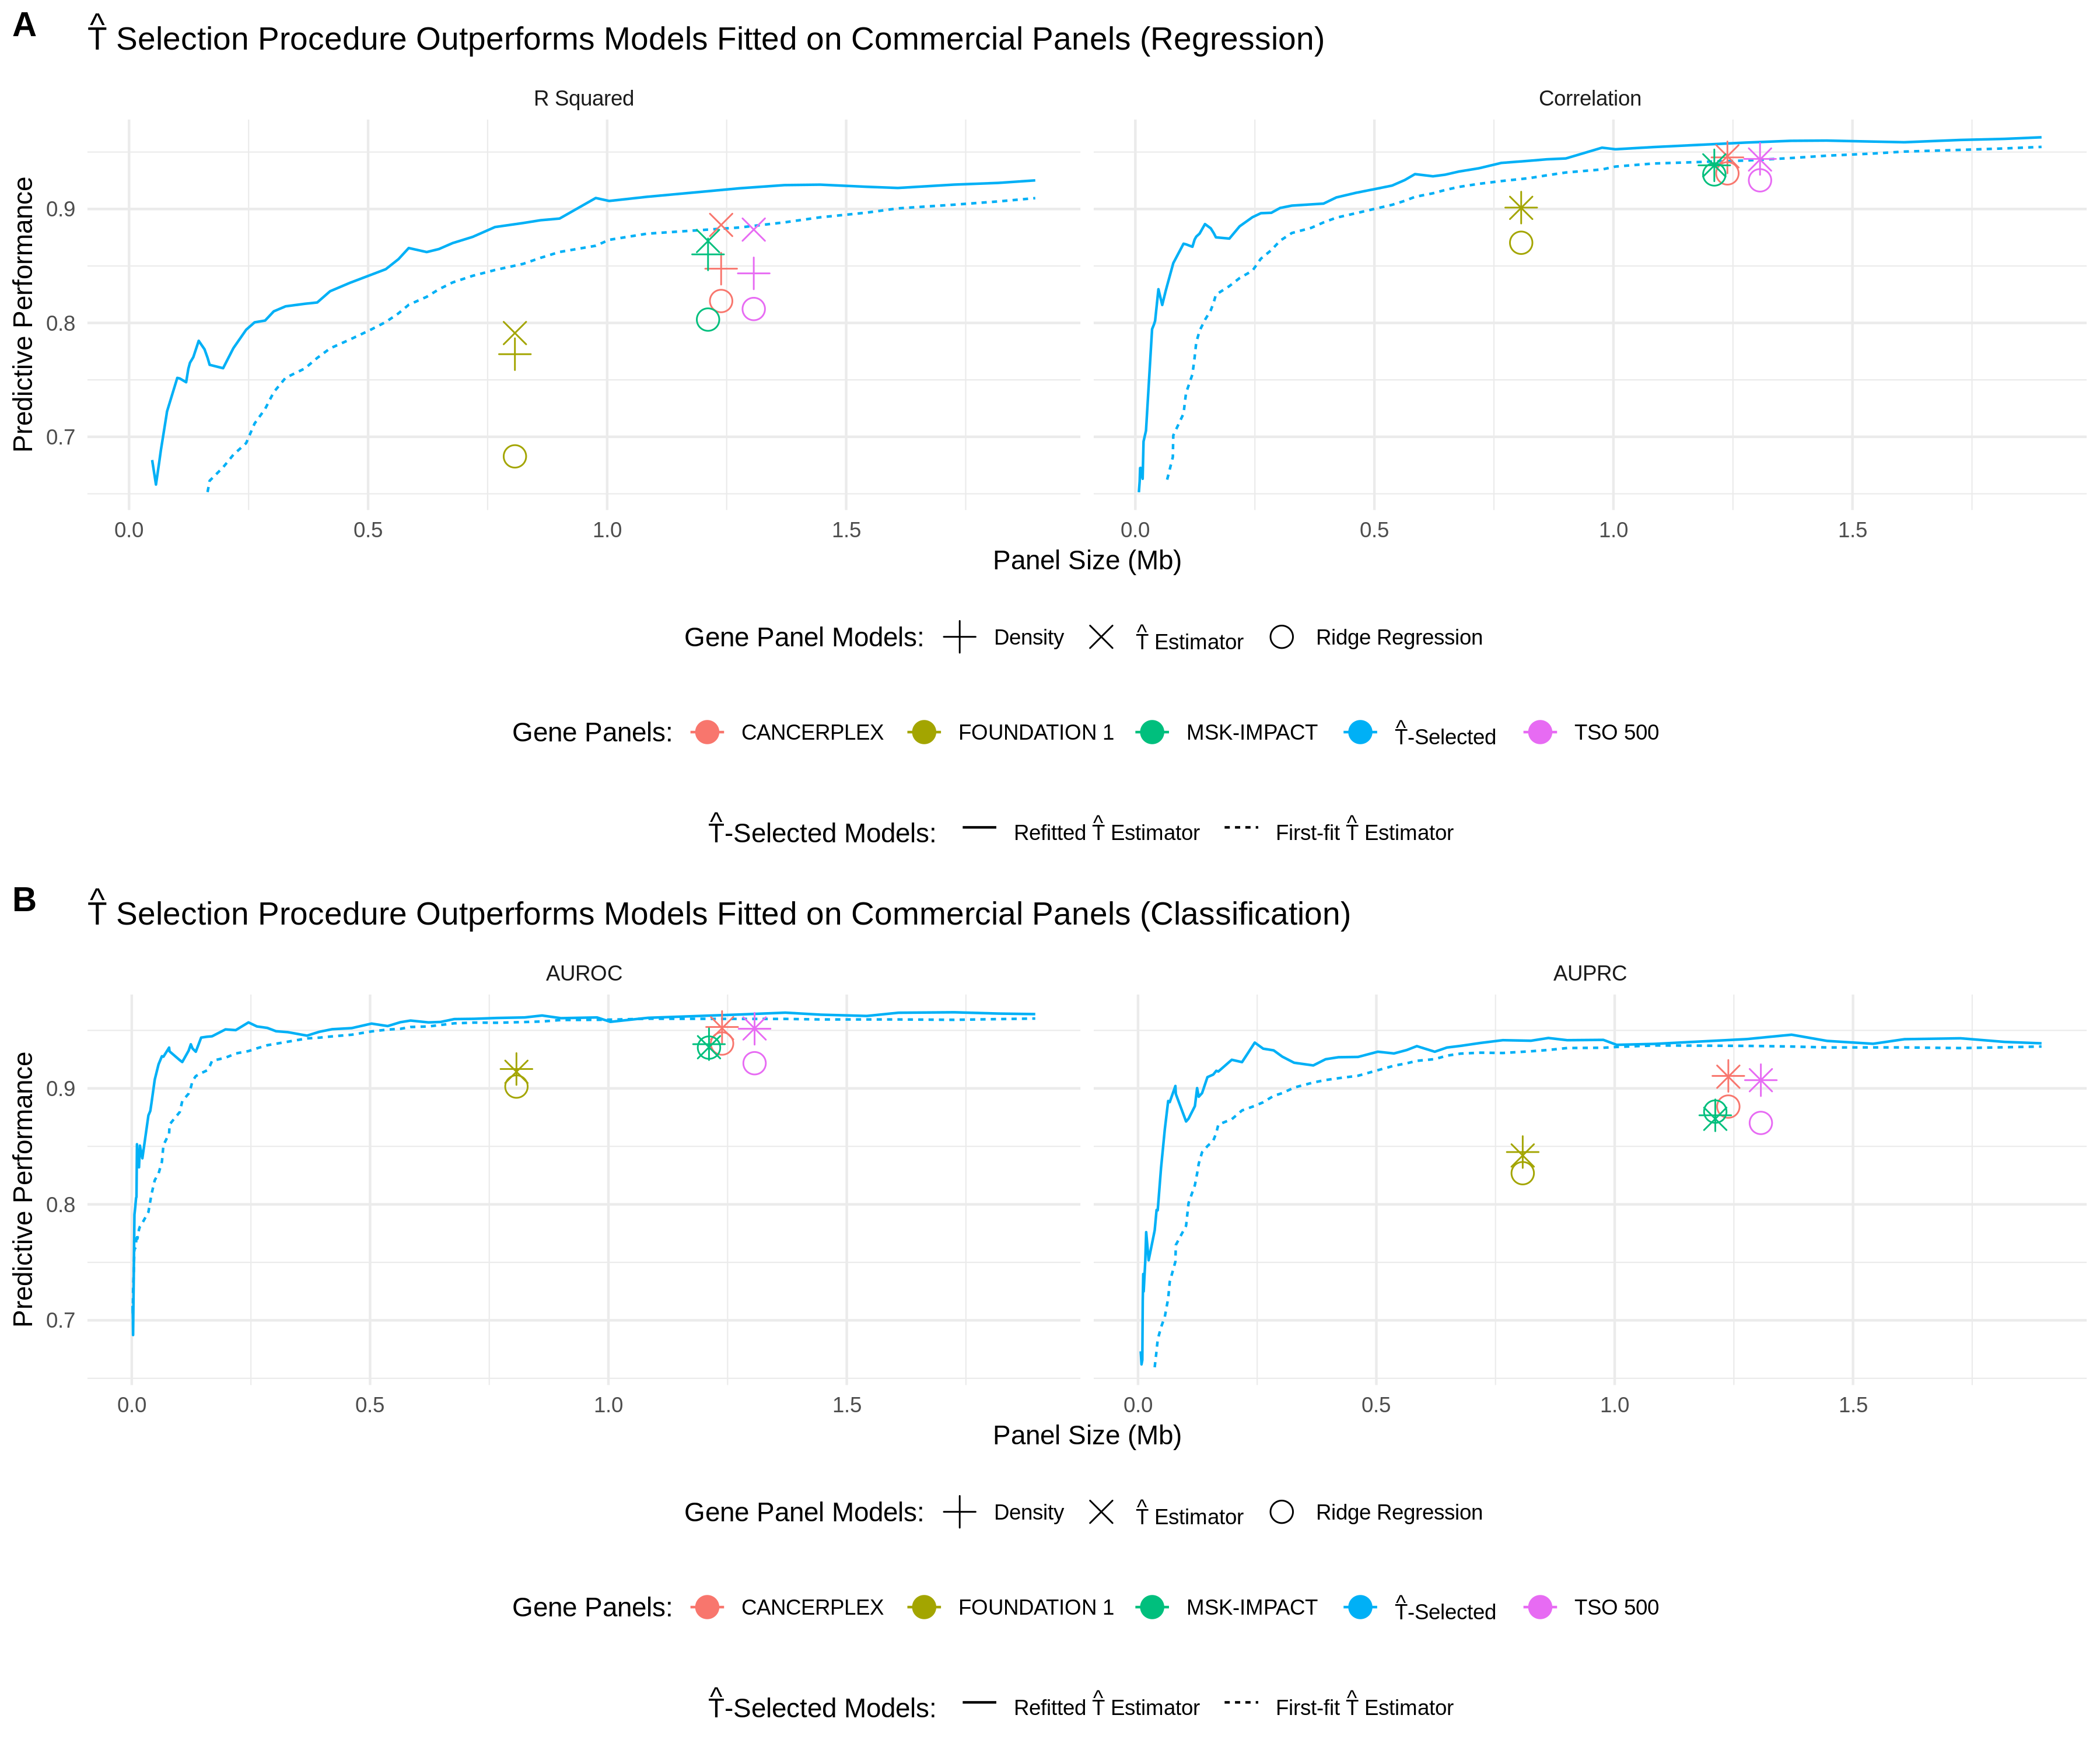
\includegraphics[width=6in]{panel_comparisons.png}
% % \caption{\jbnote{Get rid of correlation. Separate into three plots.}Comparing the predictive performance of gene panels (of varying size) selected by our methodology to commercially available gene panels. \textbf{A}: For prediction of \acrshort{tmb}, we give $R^2$ and correlation metrics. Points refer to commercial panels, with regression performed via three techniques. Lines refer to first-fit and refitted $\hat{T}$ estimators. \textbf{B}: The same comparisons for classification performance (measured by area under ROC curve and area under precision/recall curve). \label{fig:PanelComparisons}}
% % \end{figure}
% \begin{figure}[htbp]
% \centering
% 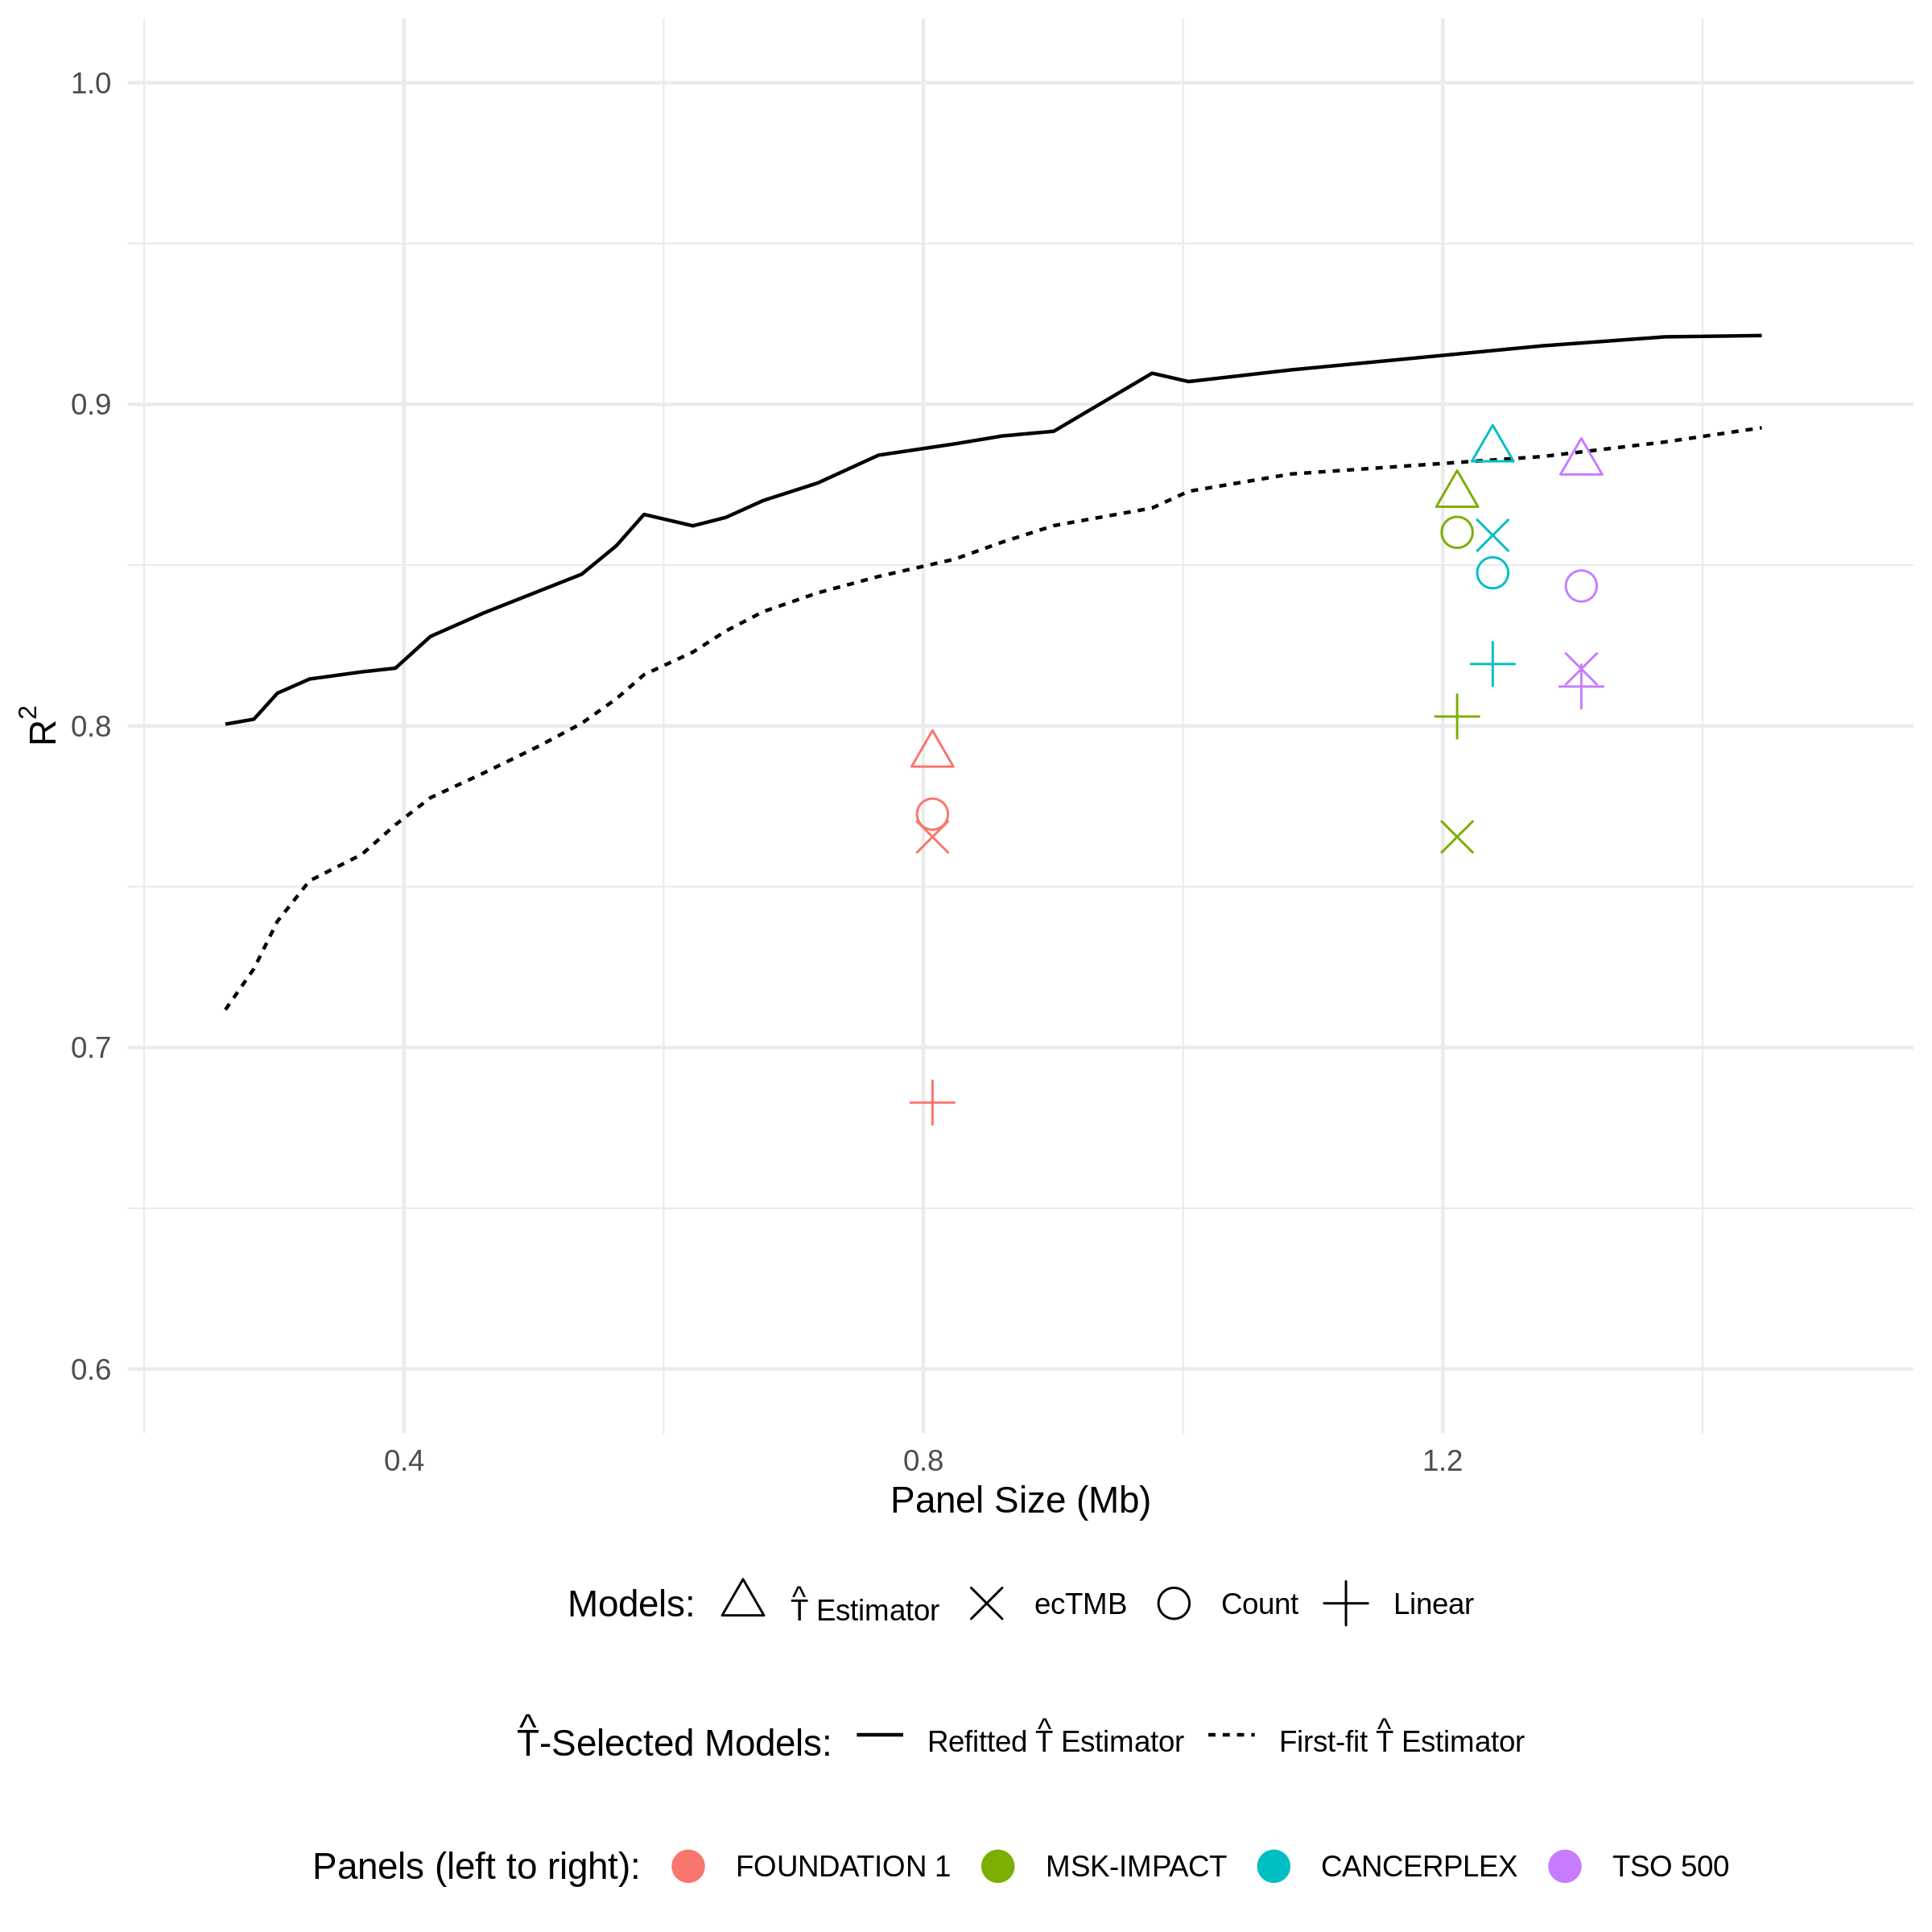
\includegraphics[width=4in]{commercial_regression_ectmb.png}
% \caption{\label{fig:commercial_regression}}
% \end{figure}

% \begin{figure}[htbp]
% \centering
% 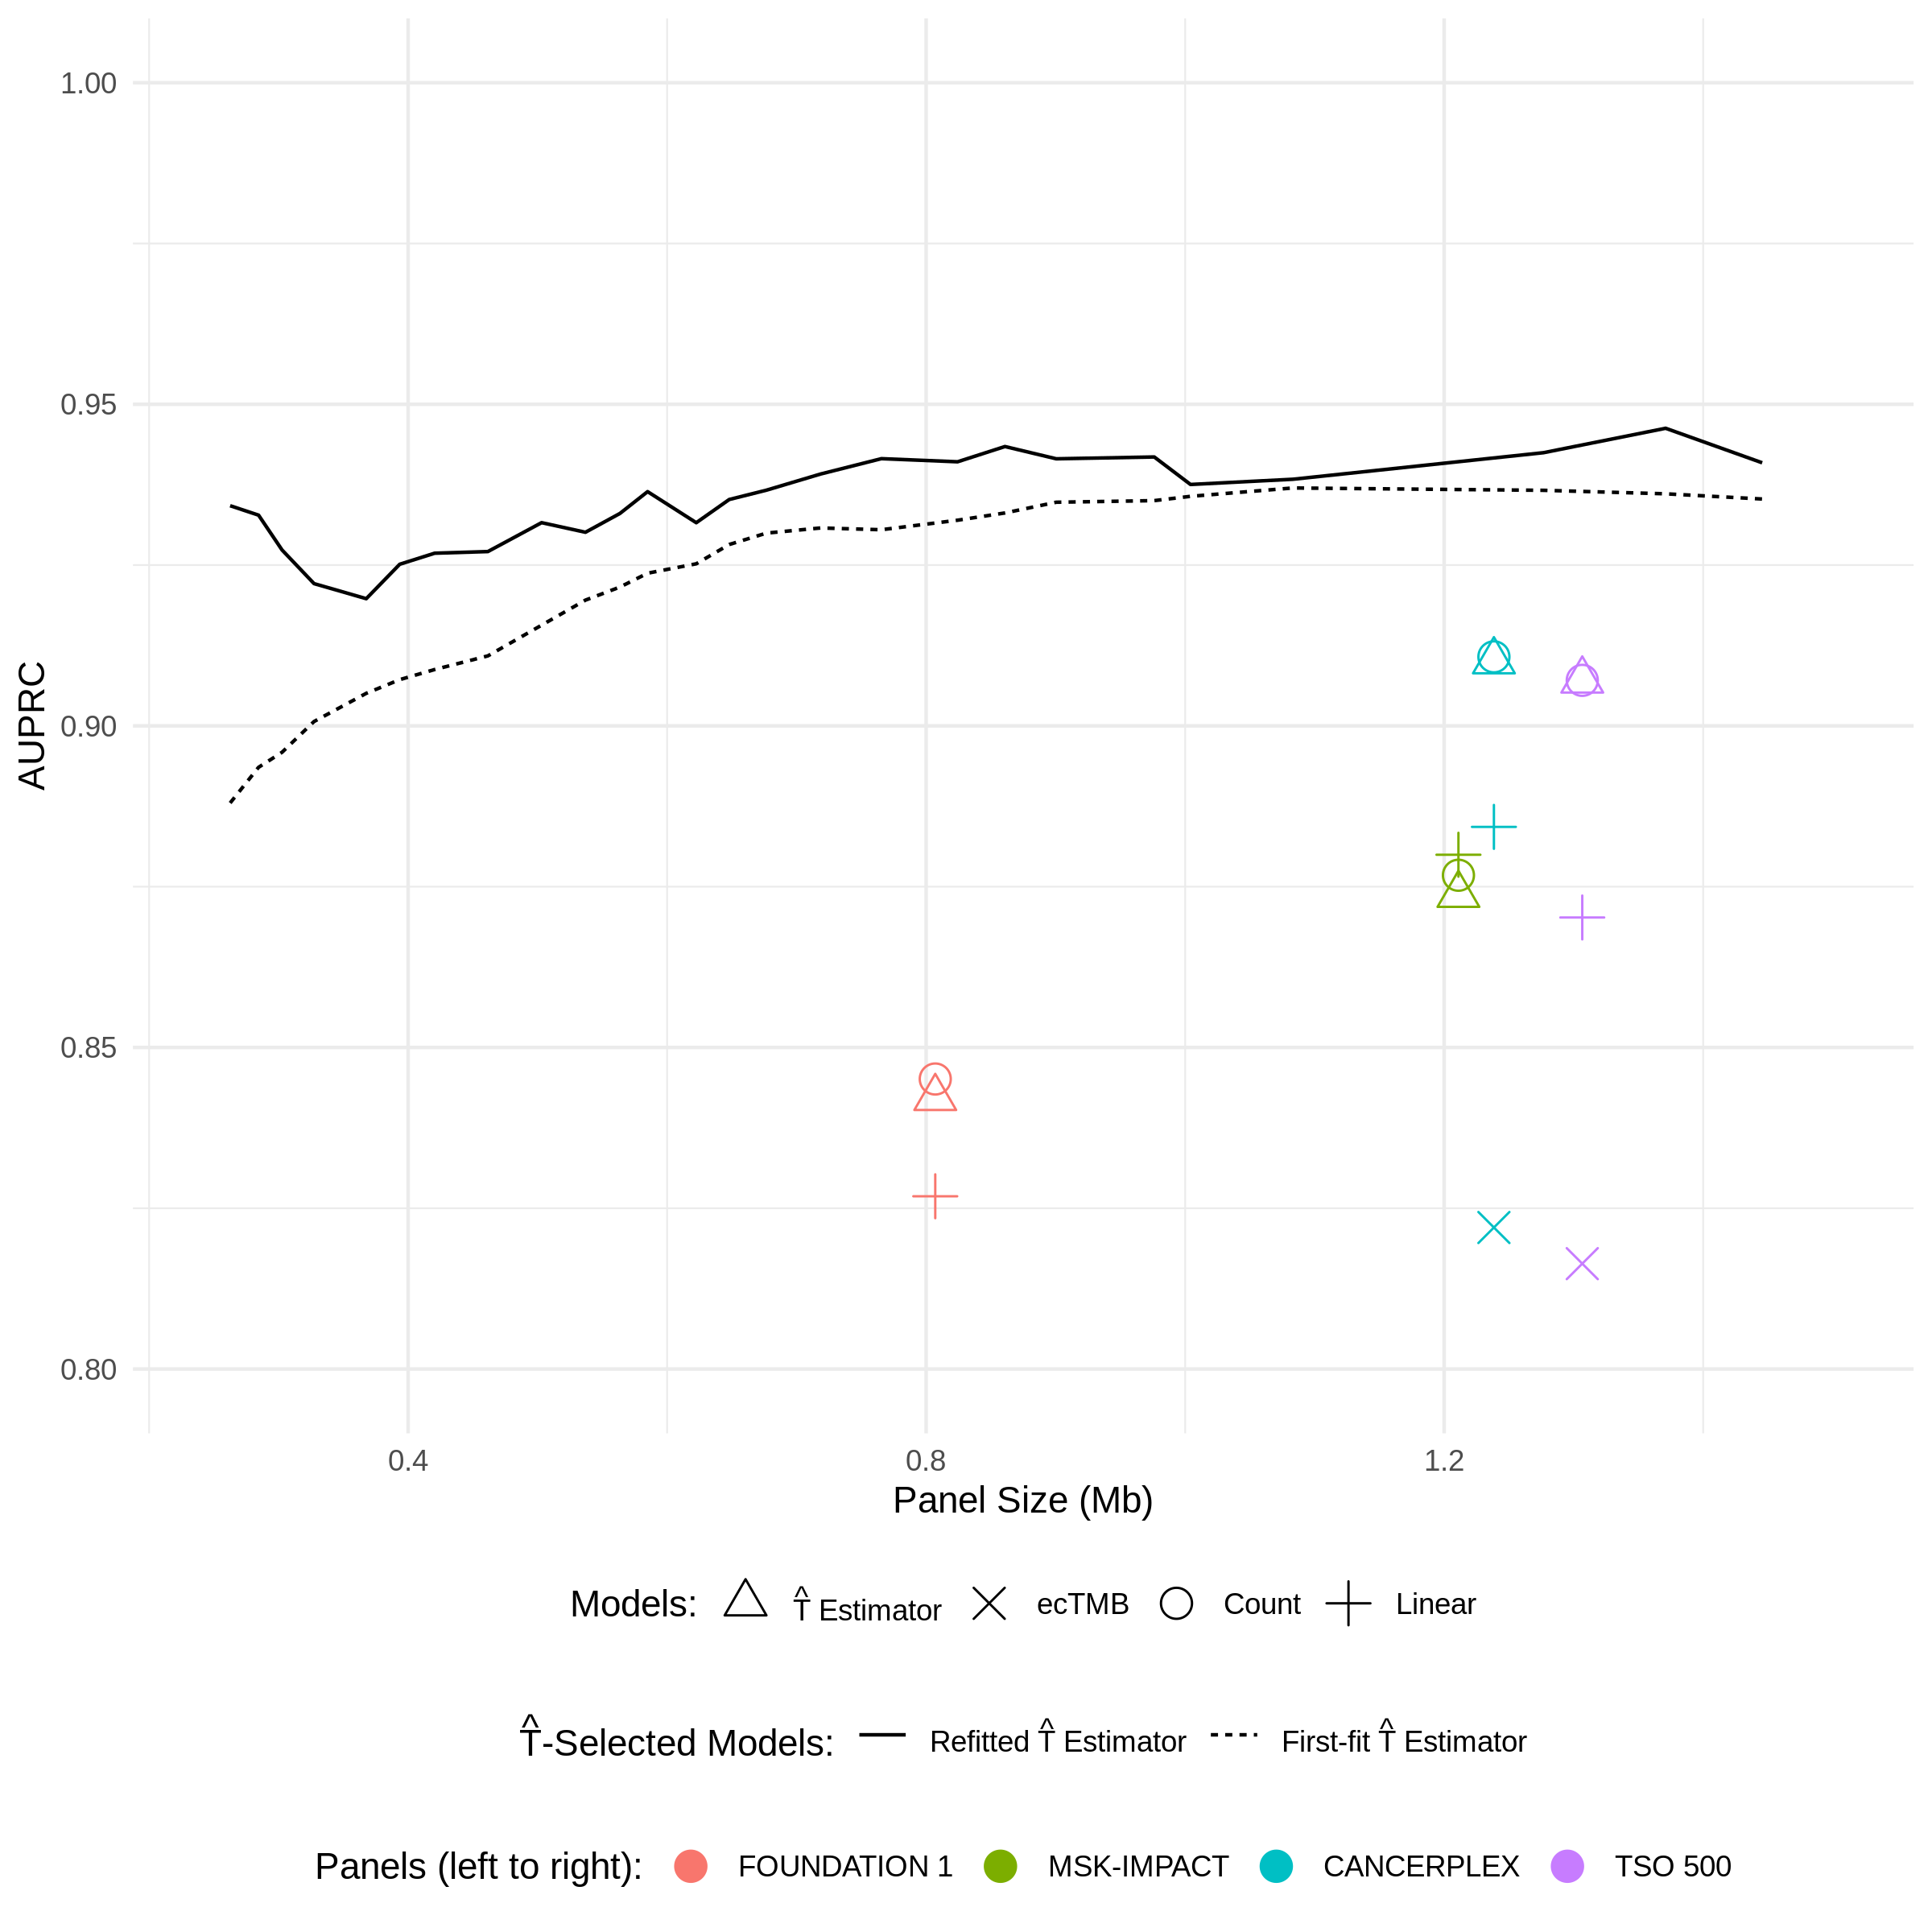
\includegraphics[width=4in]{commercial_classification_ectmb.png}
% \caption{\jbnote{cut off at 0.8, move legend to caption?}\label{fig:commercial_classification}}
% \end{figure}


\subsection{Predicting tumour indel burden \label{sec:indel}}
In this section we demonstrate how our method can be used to estimate \acrshort{tib}. 
This is more challenging than estimating \acrshort{tmb} due to the low abundance of indel mutations relative to other variant types, and issues sequencing genomic loci of repetitive nucleotide constitution \citep{narzisi_challenge_2015}. Indeed, in contrast to the previous section, we are not aware of any existing methods designed to estimate \acrshort{tib} from targeted gene panels. We therefore investigate the performance of our method across a much wider range of panel sizes in order to ascertain the feasibility of targeted \acrshort{tib} estimation. Our results demonstrate that accurate classification of \acrshort{tib} status is still possible, even though estimating the precise value of \acrshort{tib} is difficult with small panels.  

We let $S_{\text{indel}}$ be the set of all frameshift insertion and deletion mutations, and apply our method introduced in Section~\ref{sec:linearestimator} with $\bar{S} = S_{\text{indel}}$. As in the previous section, we assess regression and classification performance via $R^2$ and \acrshort{auprc}, respectively, where in this case tumours are separated into two classes: High \acrshort{tib} (more than 11 indel mutations) and Low \acrshort{tib} (otherwise). This gives 43 (25.0\%) tumours in the High \acrshort{tib} class in the validation dataset. 

\begin{figure}[htbp]
\centering
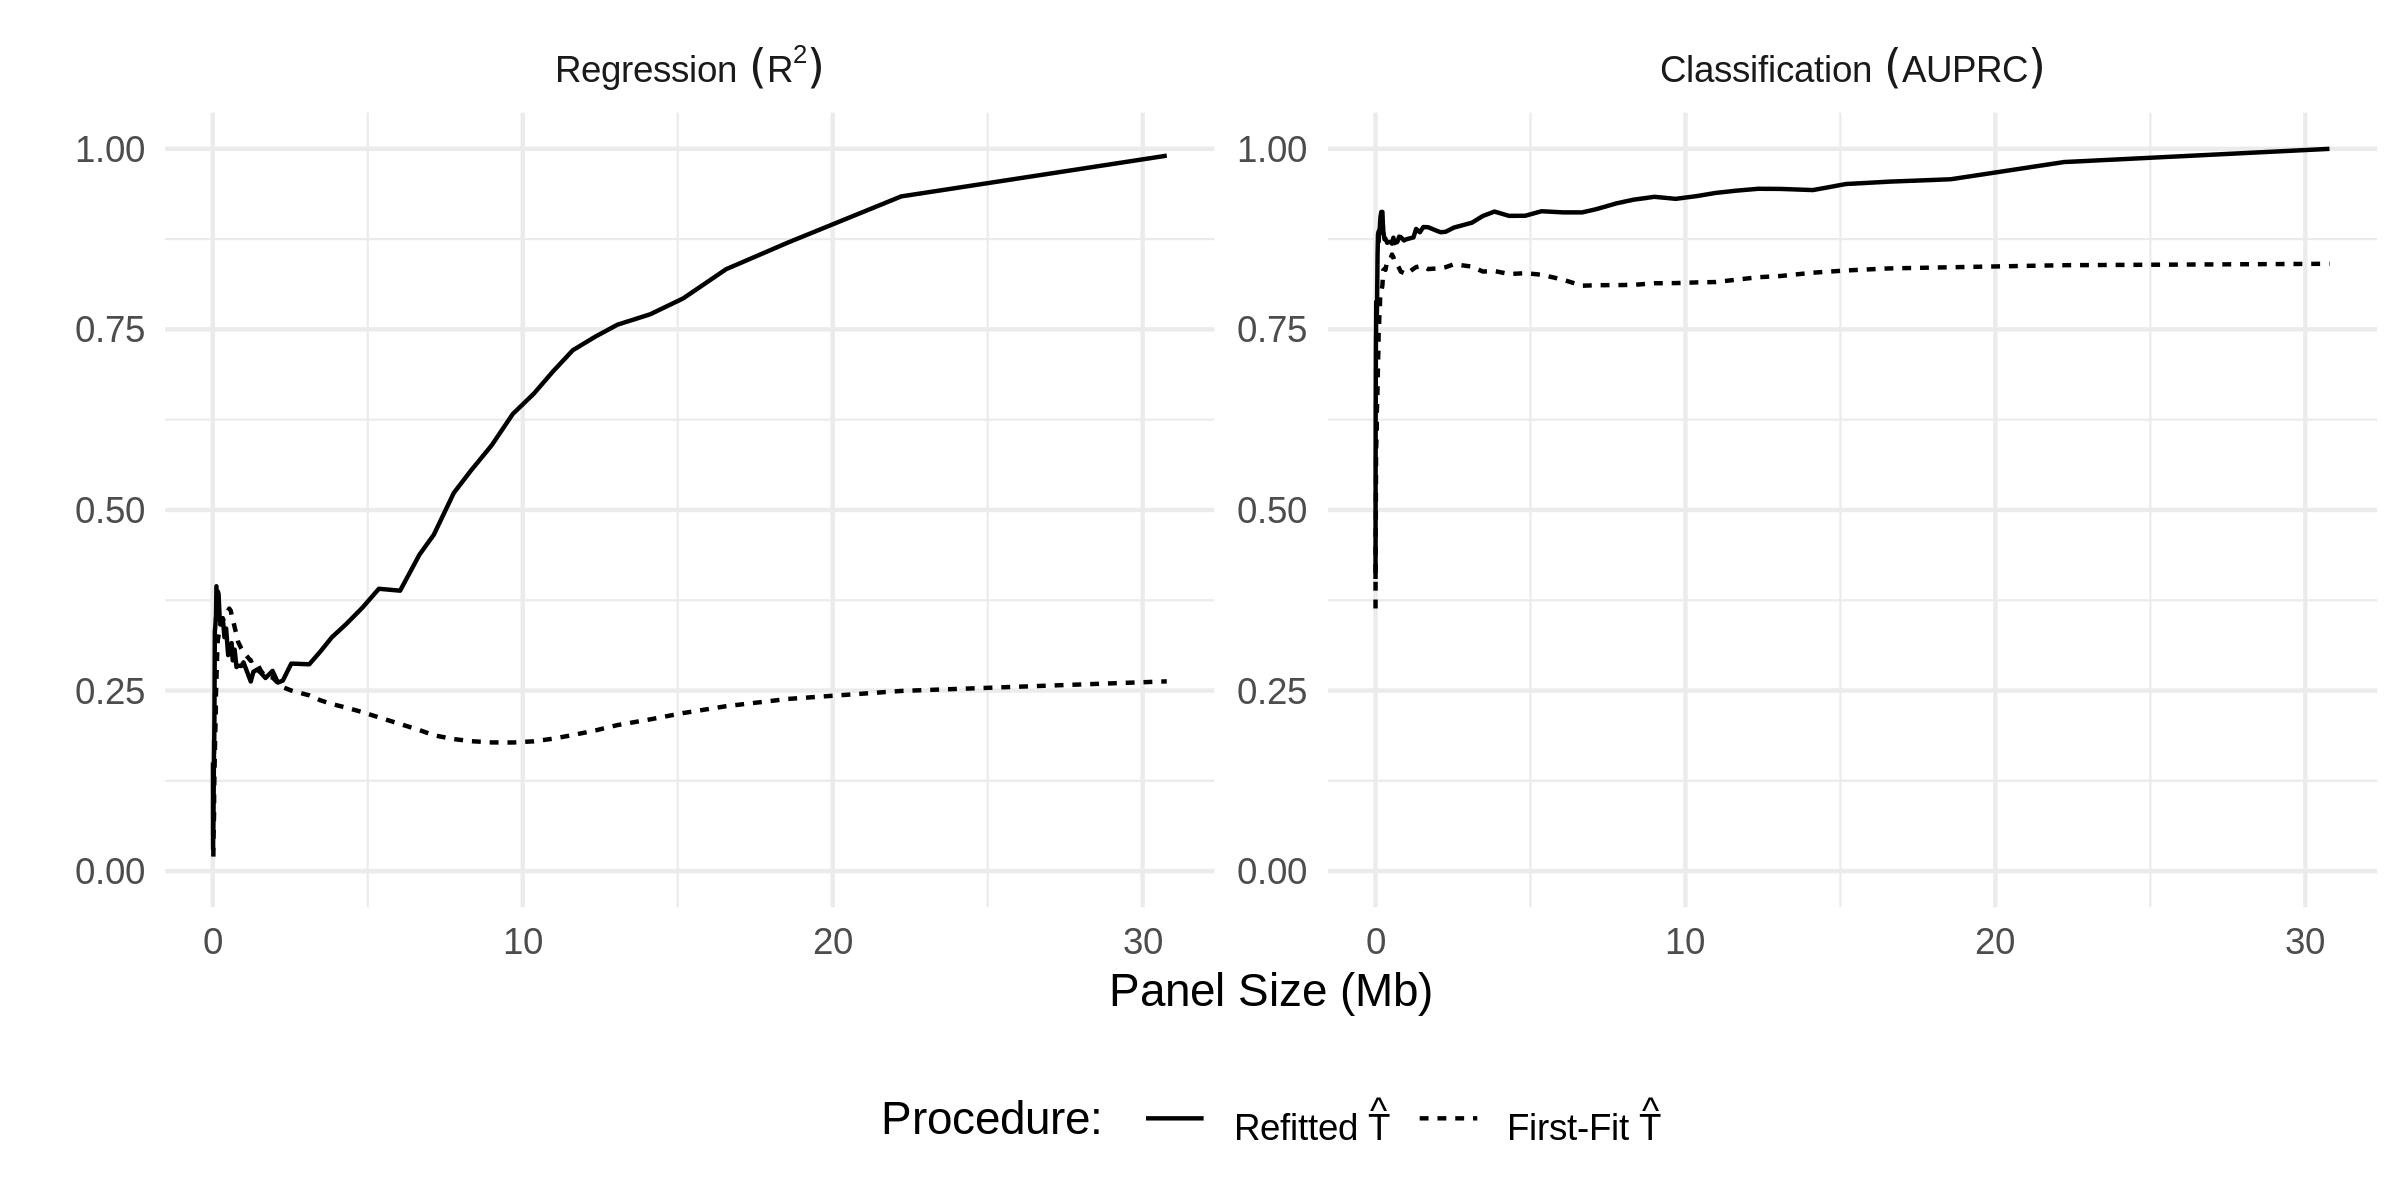
\includegraphics[width=6in]{fig9.png}
\vspace*{-5mm}
\caption{Performance of our first-fit and refitted estimators of \acrshort{tib} as the selected panel size varies. \textbf{Left}: $R^2$, \textbf{Right}: \acrshort{auprc}. \label{fig:indelstatsplot}}
\vspace*{-2mm}
\end{figure}

The results are presented in Figure \ref{fig:indelstatsplot}. We comment first on the regression performance: as expected, we see that the $R^2$ values for our first-fit and refitted estimators in this case are much lower than what we achieved in estimating \acrshort{tmb}. Perhaps surprisingly, the predictive performance of both estimators very slightly decreases as the panel size increases in the range 0.5-3.0 Mb; the refitted approach then improves for larger panel sizes. On the other hand, we see that the classification performance is impressive; our refitted method achieves an \acrshort{auprc} of 0.87 even with panel of size of~1Mb. 

\begin{figure}[htbp]
\centering
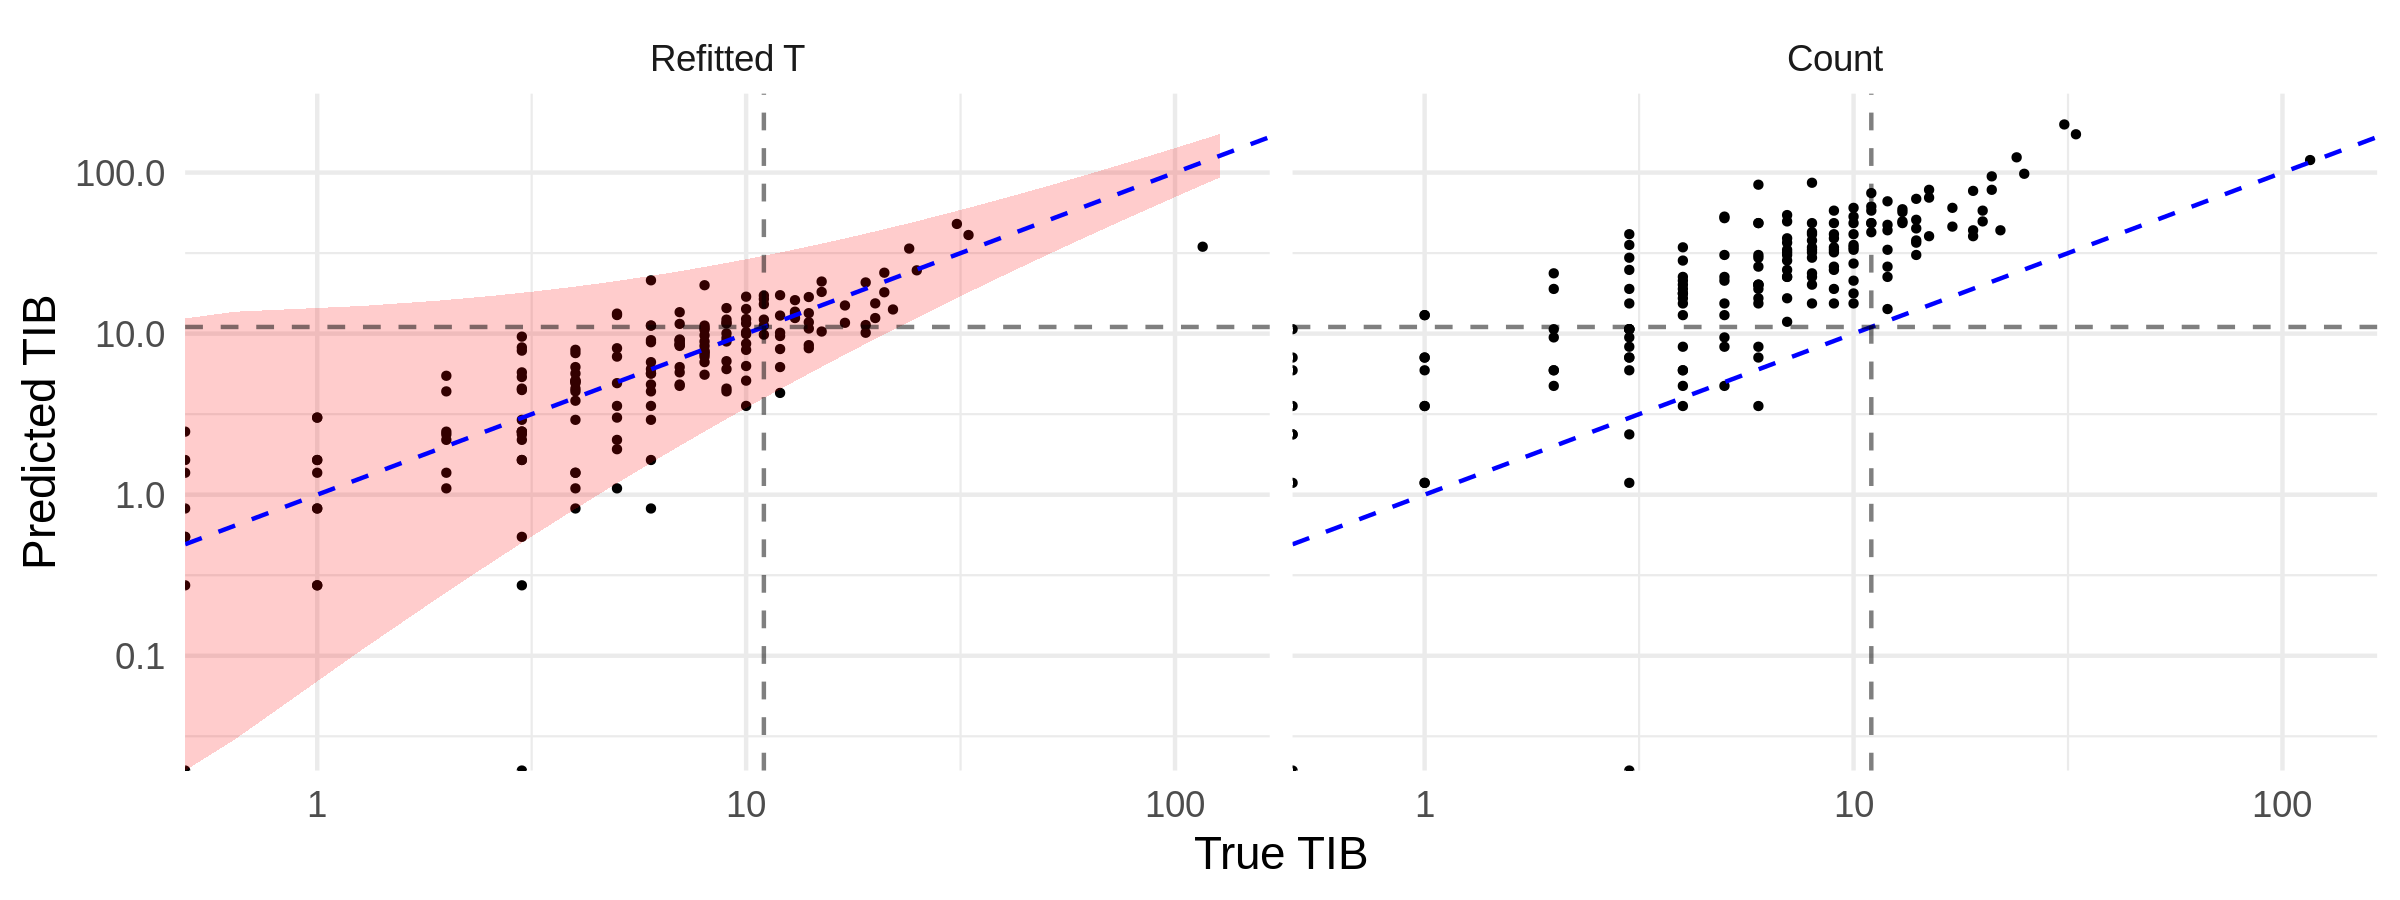
\includegraphics[width=6in]{fig10.png}
\vspace*{-5mm}
\caption{Prediction of TIB on the test dataset. Dashed blue (diagonal) line represents perfect prediction, and the grey dashed lines indicate true and predicted TIB values of 11. %Red shaded area delineates region for which 90\% prediction intervals contain truth.
\label{fig:indel_predictions_figure}}
\vspace*{-2mm}
\end{figure} 

As in the previous section, we now asses the performance on the test set of our refitted estimator of \acrshort{tib} applied to a selected panel of size~1Mb.   %and in Figure~\ref{fig:indel_predictions_figure} display the predictions of \acrshort{tib} made by the refitted estimator. 
In this case, we compare with a count estimator, which scales the total non-synonymous mutation count across the panel by the ratio of the length of the panel to that of the entire exome, and also by the relative frequency of indel mutations versus all non-synonymous mutations in the training dataset;~i.e. 
\[
\frac{\ell_G}{\ell_{P}} \frac{\sum_{i =1}^{n} \sum_{g \in G} \sum_{s \in S_{\text{indel}}} M_{igs}}{\sum_{i=1}^{n}\sum_{g \in G} \sum_{s \in S} M_{igs}}\sum_{g \in P} \sum_{s \in S} M_{0gs}.
\]
The results are presented in Figure~\ref{fig:indel_predictions_figure}. Our refitted $\hat{T}$ estimates give an $R^2$ value of 0.47 on the test set, while the count estimator again suffers from positive bias and has an $R^2$ value of -9.9. Again we include (shaded in red) the set of points for which 90\% prediction intervals contain the true value. In this case we find that 96.5\% of test set points fall within this region.

%Since there is no facility within the ecTMB procedure to predict \acrshort{tib} we do not compare with it. No linear regression procedure was found to produce estimates of \acrshort{tib} more accurate than ours (for more details see Supplementary Information \jbnote{?}). \jbnote{Exact performance of prediction intervals}.



%This elevated performance on the test set compared to the decrease in performance seen around panel sizes of 1~Mb on the validation set leads us to believe the local minimum in validation set performance is an anomalous artifact of the validation dataset (this is also borne out by the classification performance on the validation set being very high). 



\subsection{A panel-augmentation case study \label{sec:augmentation}}
As discussed in Section \ref{sec:panelaugmentation}, we may wish to include genes from a given panel, but use our methodology to augment the panel to include a small set of additional genes in order to obtain more accurate predictions of \acrshort{tmb}. In this section we demonstrate how this can be done starting with the Foundation~1 panel, which contains 324 genes (approximately 0.8Mb). We will see that, by increasing the panel to 1Mb in size using our proposal, we can significantly improve the predictive performance. 

\begin{table}[ht]
\begin{center}
\caption{Predictive performance of models on Foundation~1 (0.8Mb) versus augmented Foundation~1 (1.0Mb) panels (test set). \jbnote{This will need to be looked at again when the code is re-run}  \label{table:augpanel}}
\begin{tabular}{ | c | c | c | c | c |}
\hline
\multirow{2}{*}{Model} & \multicolumn{2}{c |}{Regression ($R^2$)} & \multicolumn{2}{c|}{Classification (AUPRC)}  \\
\cline{2-5}
  & Foundation  & Augmented  & Foundation  & Augmented    \\
 \hline
Refitted $\hat{T}$ & 0.69 & 0.82 & 0.80  &  0.91       \\
% ecTMB  & 0.76 & 0.80 & 0.82 & 0.79  \\
% Count & 0.61 & -0.54 & 0.79 & 0.91 \\
% Linear & 0.58 & 0.62 & 0.73  & 0.84 \\
\hline

\end{tabular}
\vspace*{-5mm}
\end{center}
\end{table}

We apply the augmentation method described in Section~\ref{sec:panelaugmentation}, with $P_0$ taken to be Foundation~1 genes and set $Q_0$ to be empty.  The genes added to the panel are determined by the first-fit estimator in equation~\eqref{eq:augment}. To evaluate the performance, we then apply the refitted estimator on the test dataset, after selecting the augmented panel of size 1Mb. For comparison, we apply our refitted estimator to the Foundation~1 panel directly. We also present the results obtained by the other estimators described above, both before and after the panel augmentation, in Table~\ref{table:augpanel}. We find that the augmented panel produces enhanced predictive performance under the refitted $\hat{T}$ estimator in regression and classification. The refitted estimator provides better estimates than any other model on the augmented panel by both metrics. Notably, the ecTMB and count estimators suffer weakened results on the augmented panel (the count estimator at regression, ecTMB at classification). While augmenting a gene panel can produce enhanced results, it appears that this (perhaps unsurprisingly) may only be the case when employing an estimator designed in conjunction with the panel selection procedure.

%our proposed workflow in comparison with existing methodology, we began with the Foundation~1 panel, a collection of around 300 genes with a total footprint $\approx$ 0.8Mb. The genes included in the panel have been identified as cancer-relevant or driver genes.

%We augment this gene list via the procedure described in Section \ref{sec:practicalconsiderations} to produce a panel of length of 1Mb. This selection is done by optimising for prediction of tumour indel burden, as this is in general a harder problem than estimation of tumour mutation burden. Based on this selection we can produce linear estimators for \acrshort{tmb} and \acrshort{tib}, and we present results of applying these estimators to an unseen test set of 172 samples in Figure \ref{fig:augpanel}. 

% \begin{figure}[htbp]
% \centering
% 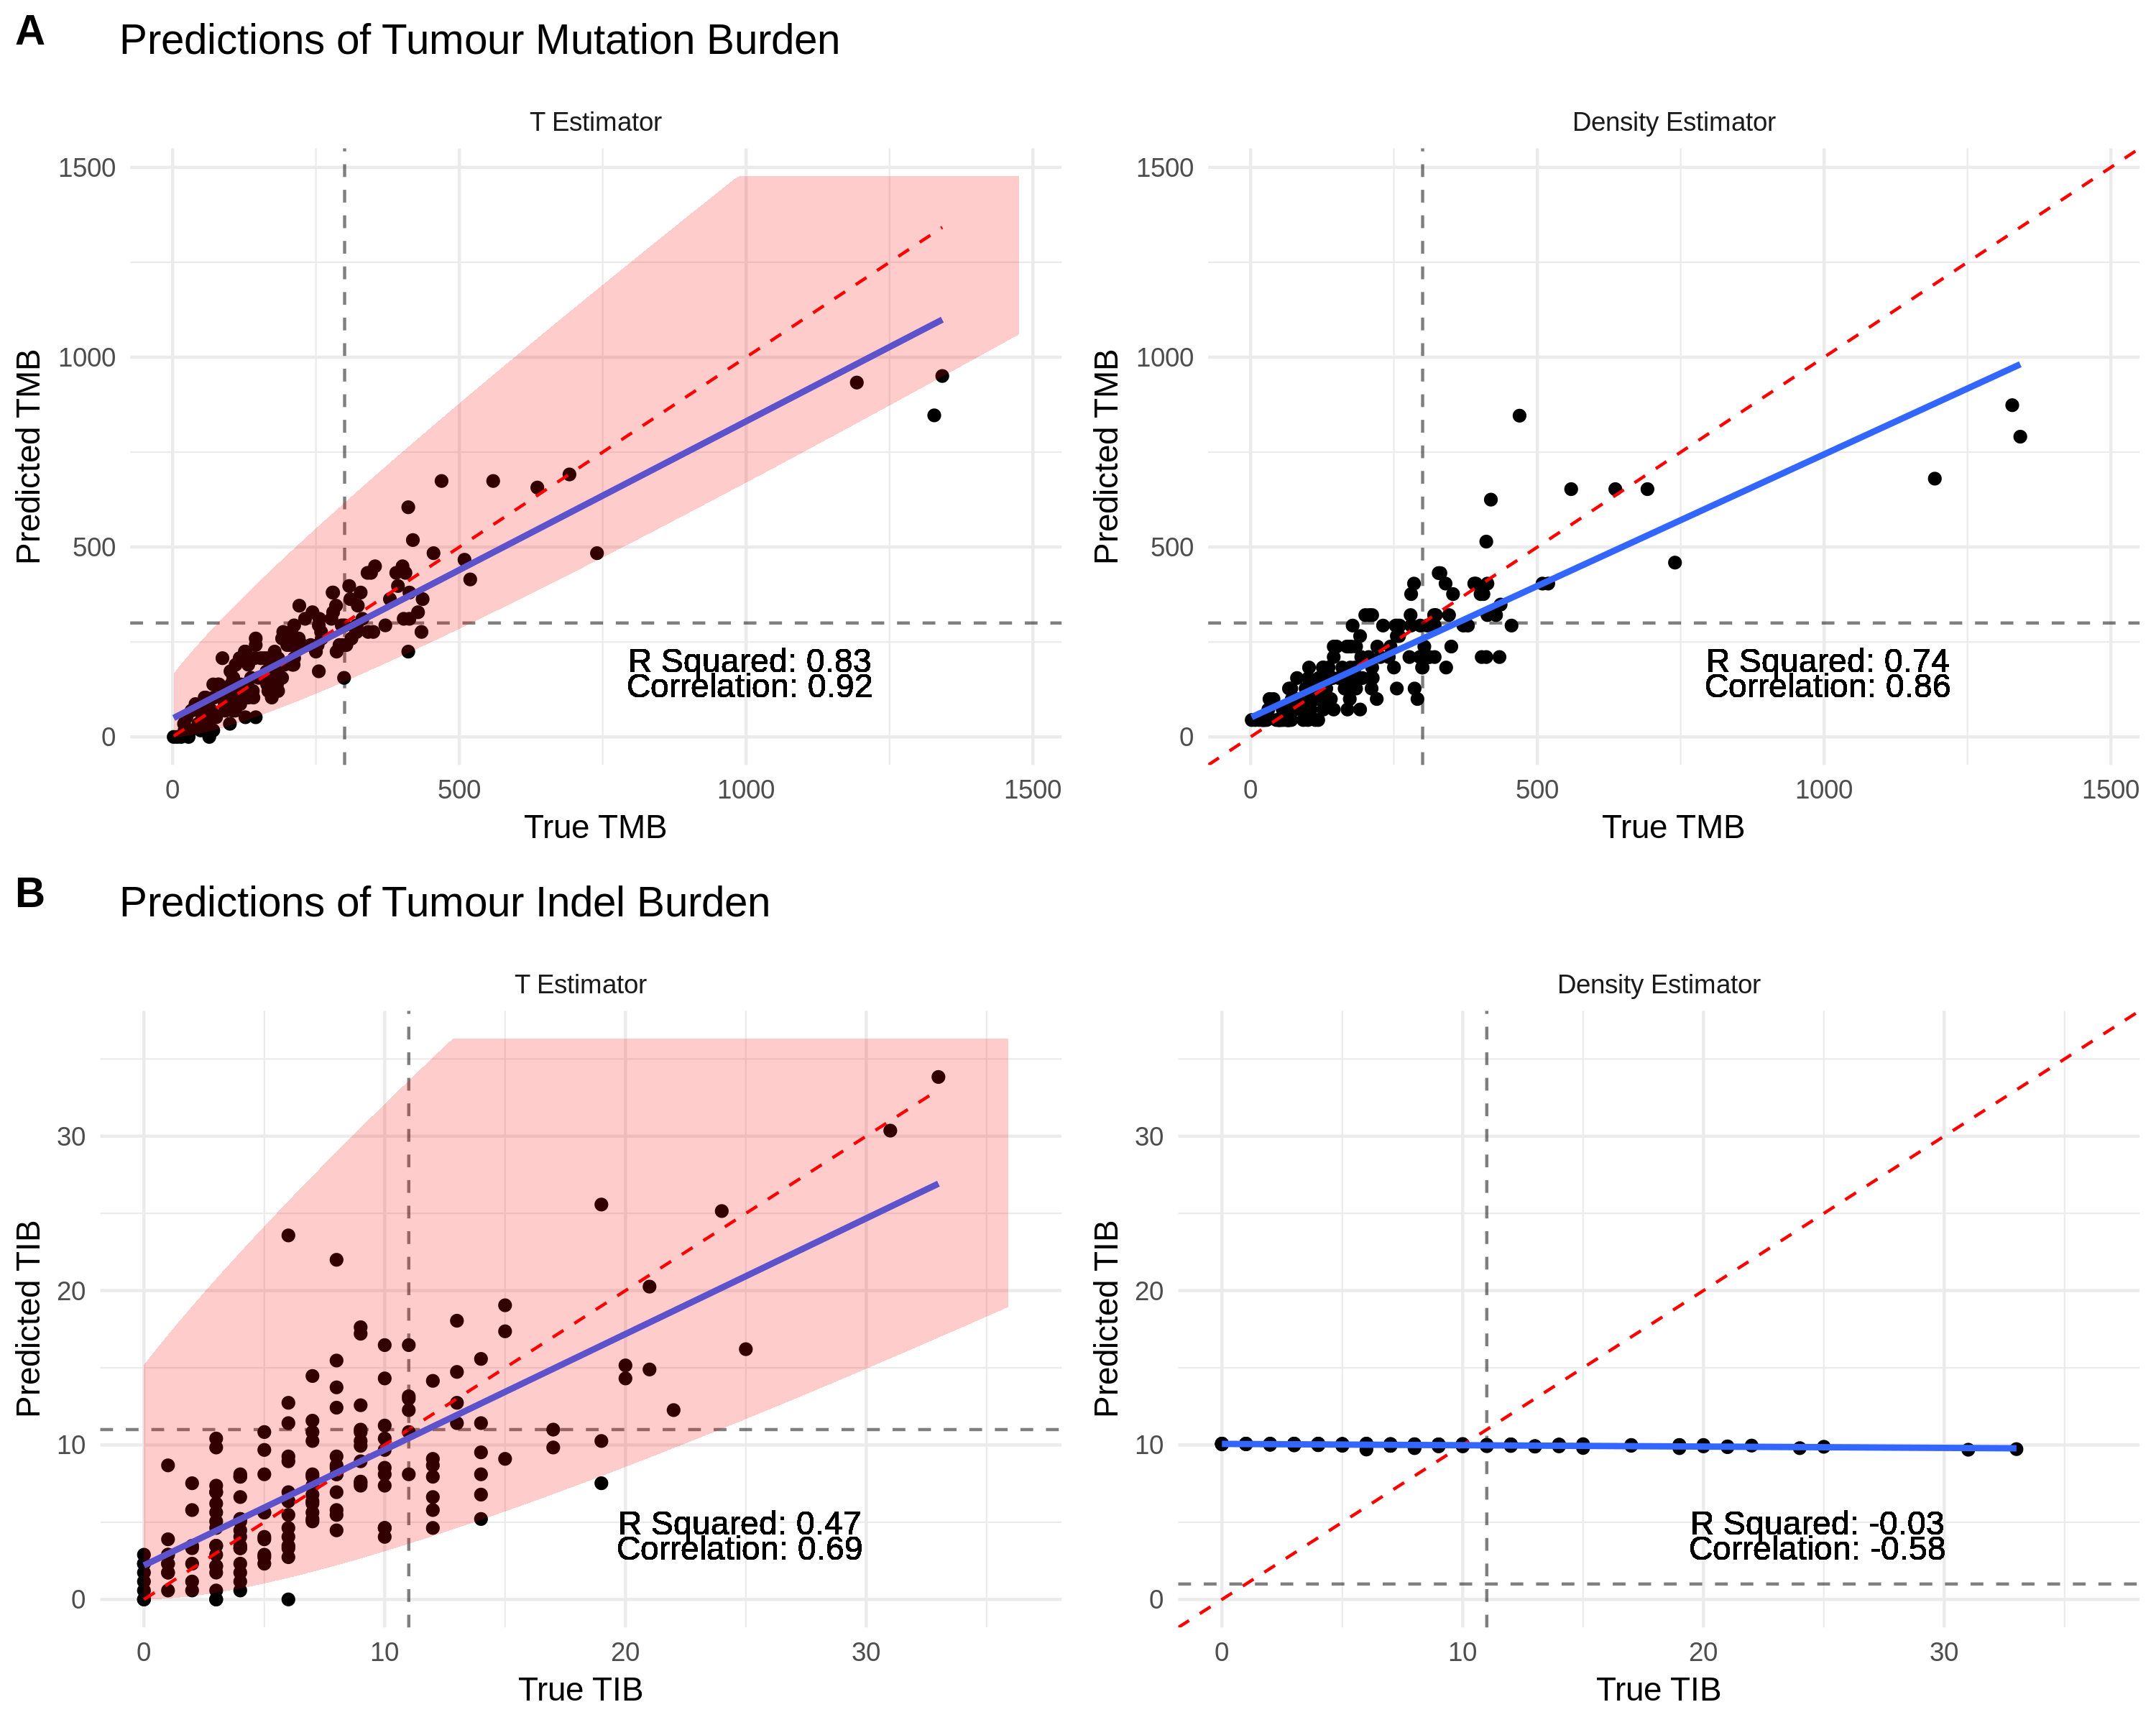
\includegraphics[width=6in]{aug_panel_output.png}
% \caption{\textbf{A}: Predictions of \acrshort{tmb} from an augmented 1Mb gene panel. The left figure compares predicted and true values for our estimator, with the shaded red area showing points for which the true value is contained within a 90\% confidence interval of the predicted value. A line of best fit is given in blue, and dashed lines indicate (in black) our classification thresholds and (in red) perfect predictions. The right figure shows the same comparisons for a density-based estimator on non-Foundation genes. \textbf{B}: The same comparisons as in \textbf{A}, but for the prediction of \acrshort{tib}. One sample with particularly high \acrshort{tib} (120) is excluded. \label{fig:augpanel}}
% \end{figure} 

%Since the genes in the Foundation One panel are selected to be cancer drivers, standard methodology would currently dictate that they be excluded from use in prediction. As a comparison therefore, we use density-based estimates calculated from the 0.2Mb of non-Foundation genomic space selected by our augmentation procedure. To make the comparison fair, we allowed the density estimates to be scaled by a linear factor that was learned from the training dataset. We see in Figure \ref{fig:augpanel}\textbf{A} that our estimator does indeed outperform the density-based estimator at prediction, with the additional bonus that we are able to provide error bounds. As would be expected, performance for prediction of \acrshort{tib} is substantially lower (Figure \ref{fig:augpanel}\textbf{B}). However, in this case a density-based estimator is unable to detect meaningful signal.

% \begin{figure}[htbp]
% \centering
% 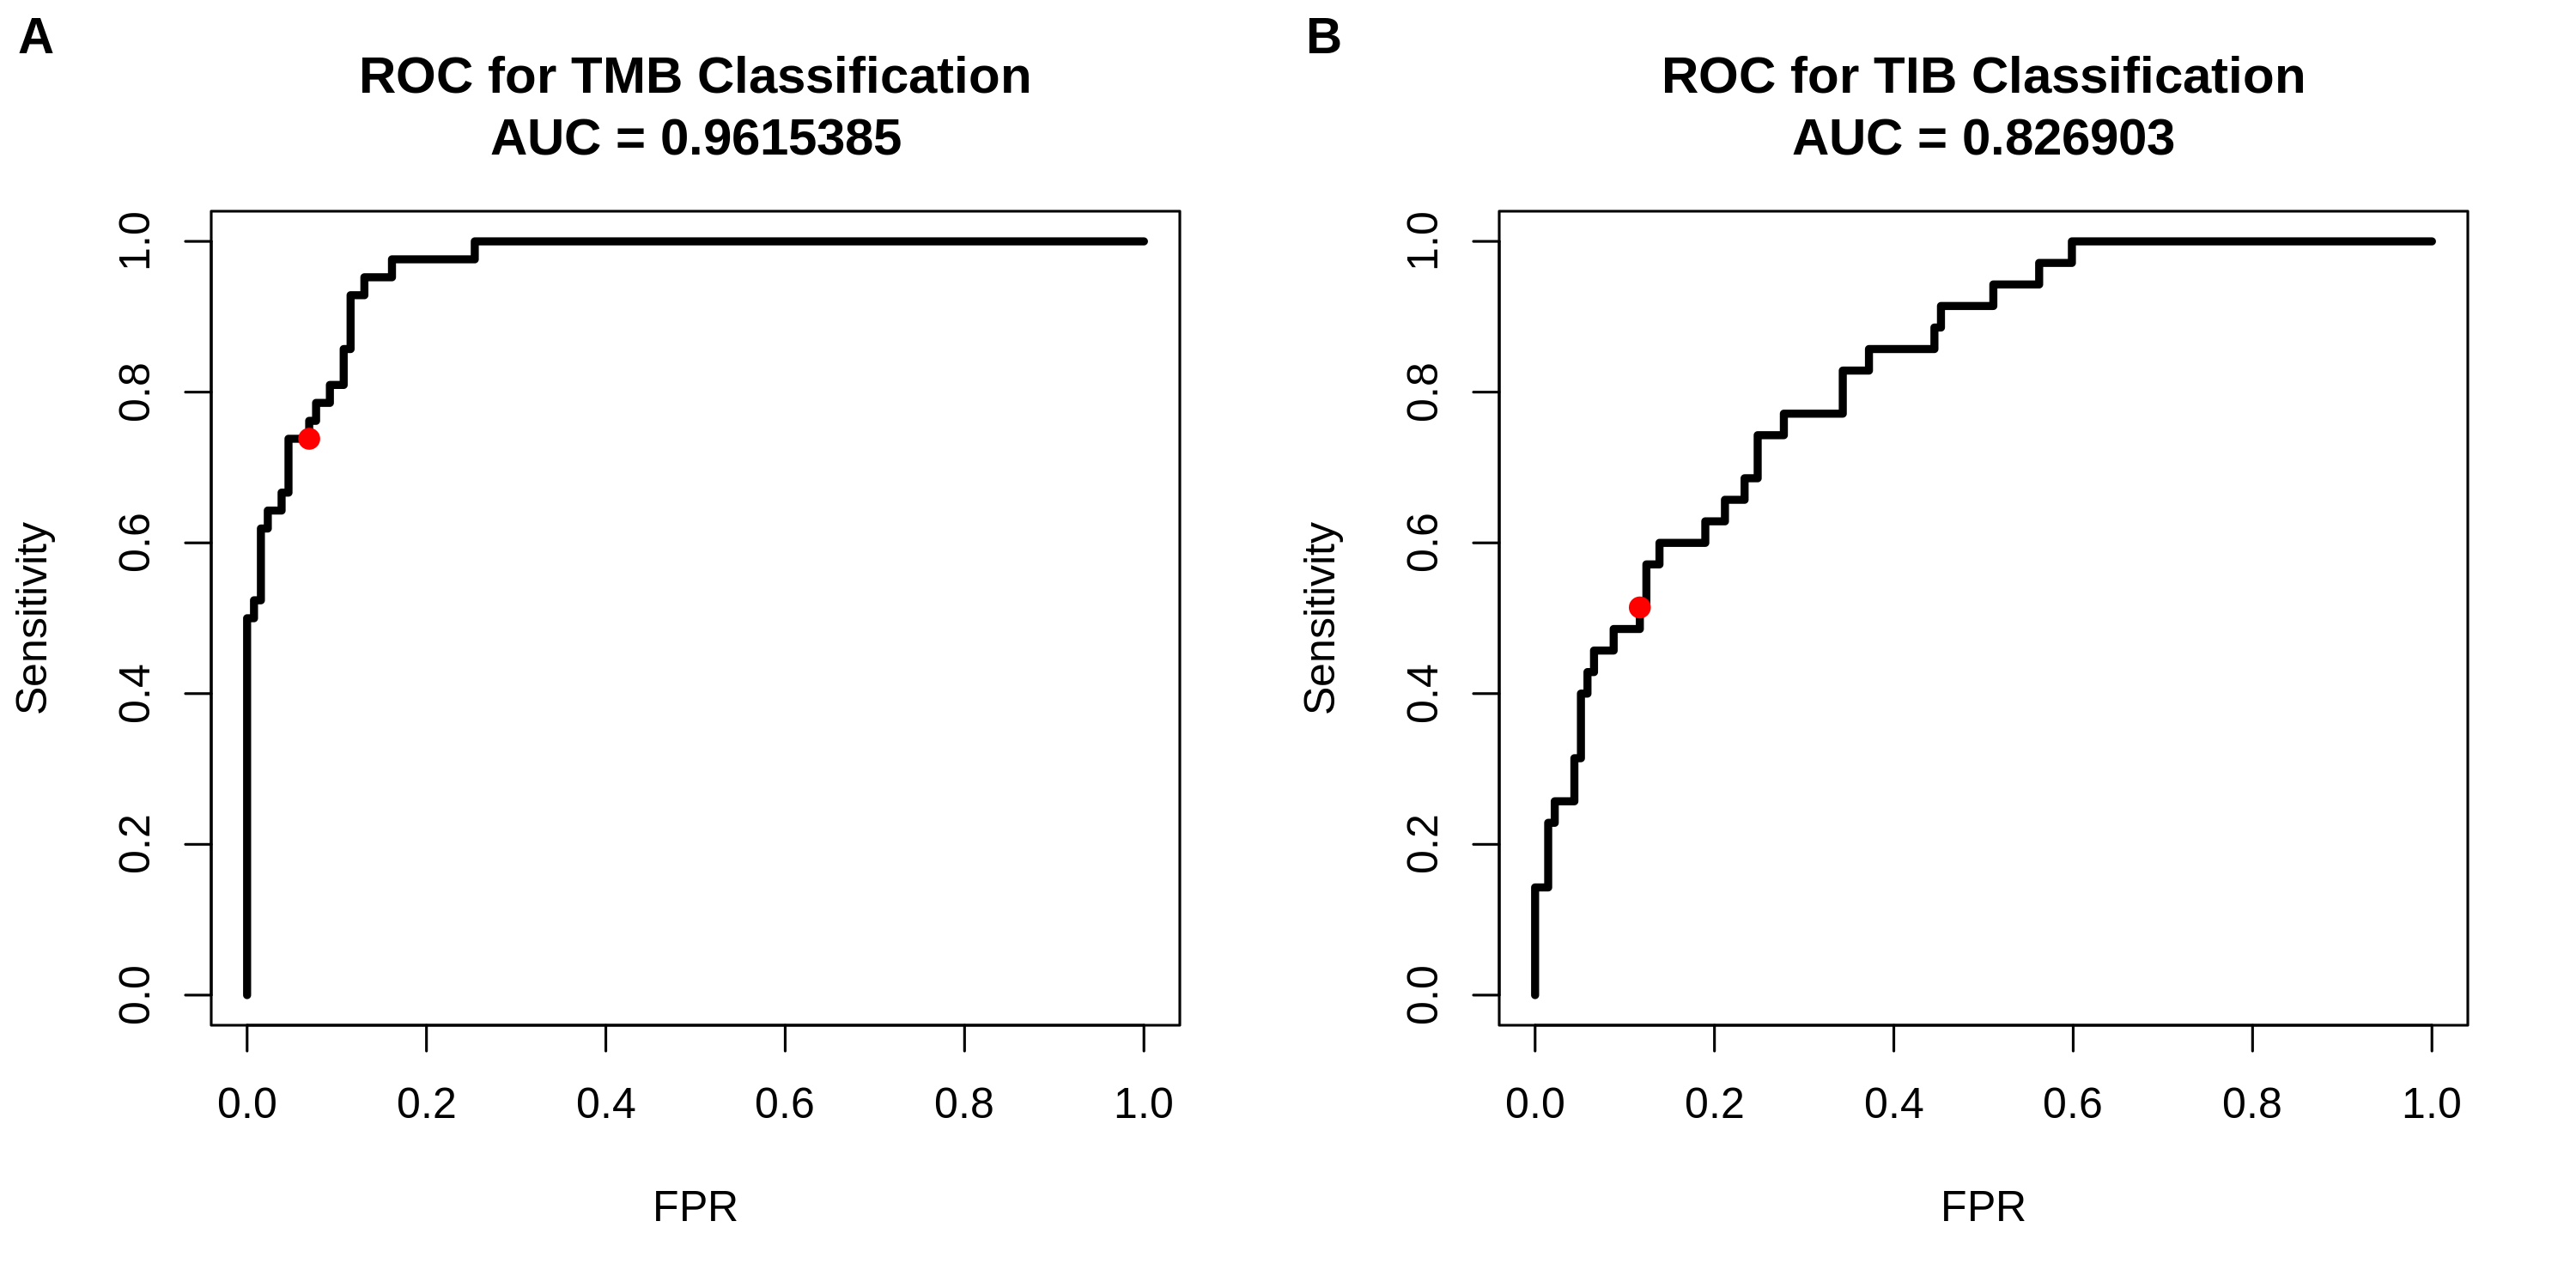
\includegraphics[width=6in]{aug_panel_aucs.png}
% \caption{\jbnote{Change this to PRC} Receiver Operator Characteristic (ROC curves) for \textbf{A}: classification of \acrshort{tmb}-High/Low (threshold 300 mutations), \textbf{B}: classification of \acrshort{tib}-High/Low (threshold of 11 mutations).  \label{fig:augpanelaucs}}
% \end{figure}

% For the augmented panel, we produced ROC plots for classification of \acrshort{tmb} and \acrshort{tib} (shown in Figure \ref{fig:augpanelaucs}). To vary the sensitivity and false positive rate we altered the predictive threshold (while maintaining the threshold for true class labels constant). The red points in Figures \ref{fig:augpanelaucs}\textbf{A} and \ref{fig:augpanelaucs}\textbf{B} refer to classifiers where the predictive threshold is chosen to be the same as the true class threshold. We see excellent overall classification for \acrshort{tmb} and promising performance for \acrshort{tib}.
% \begin{figure}[htbp]
% \centering
% 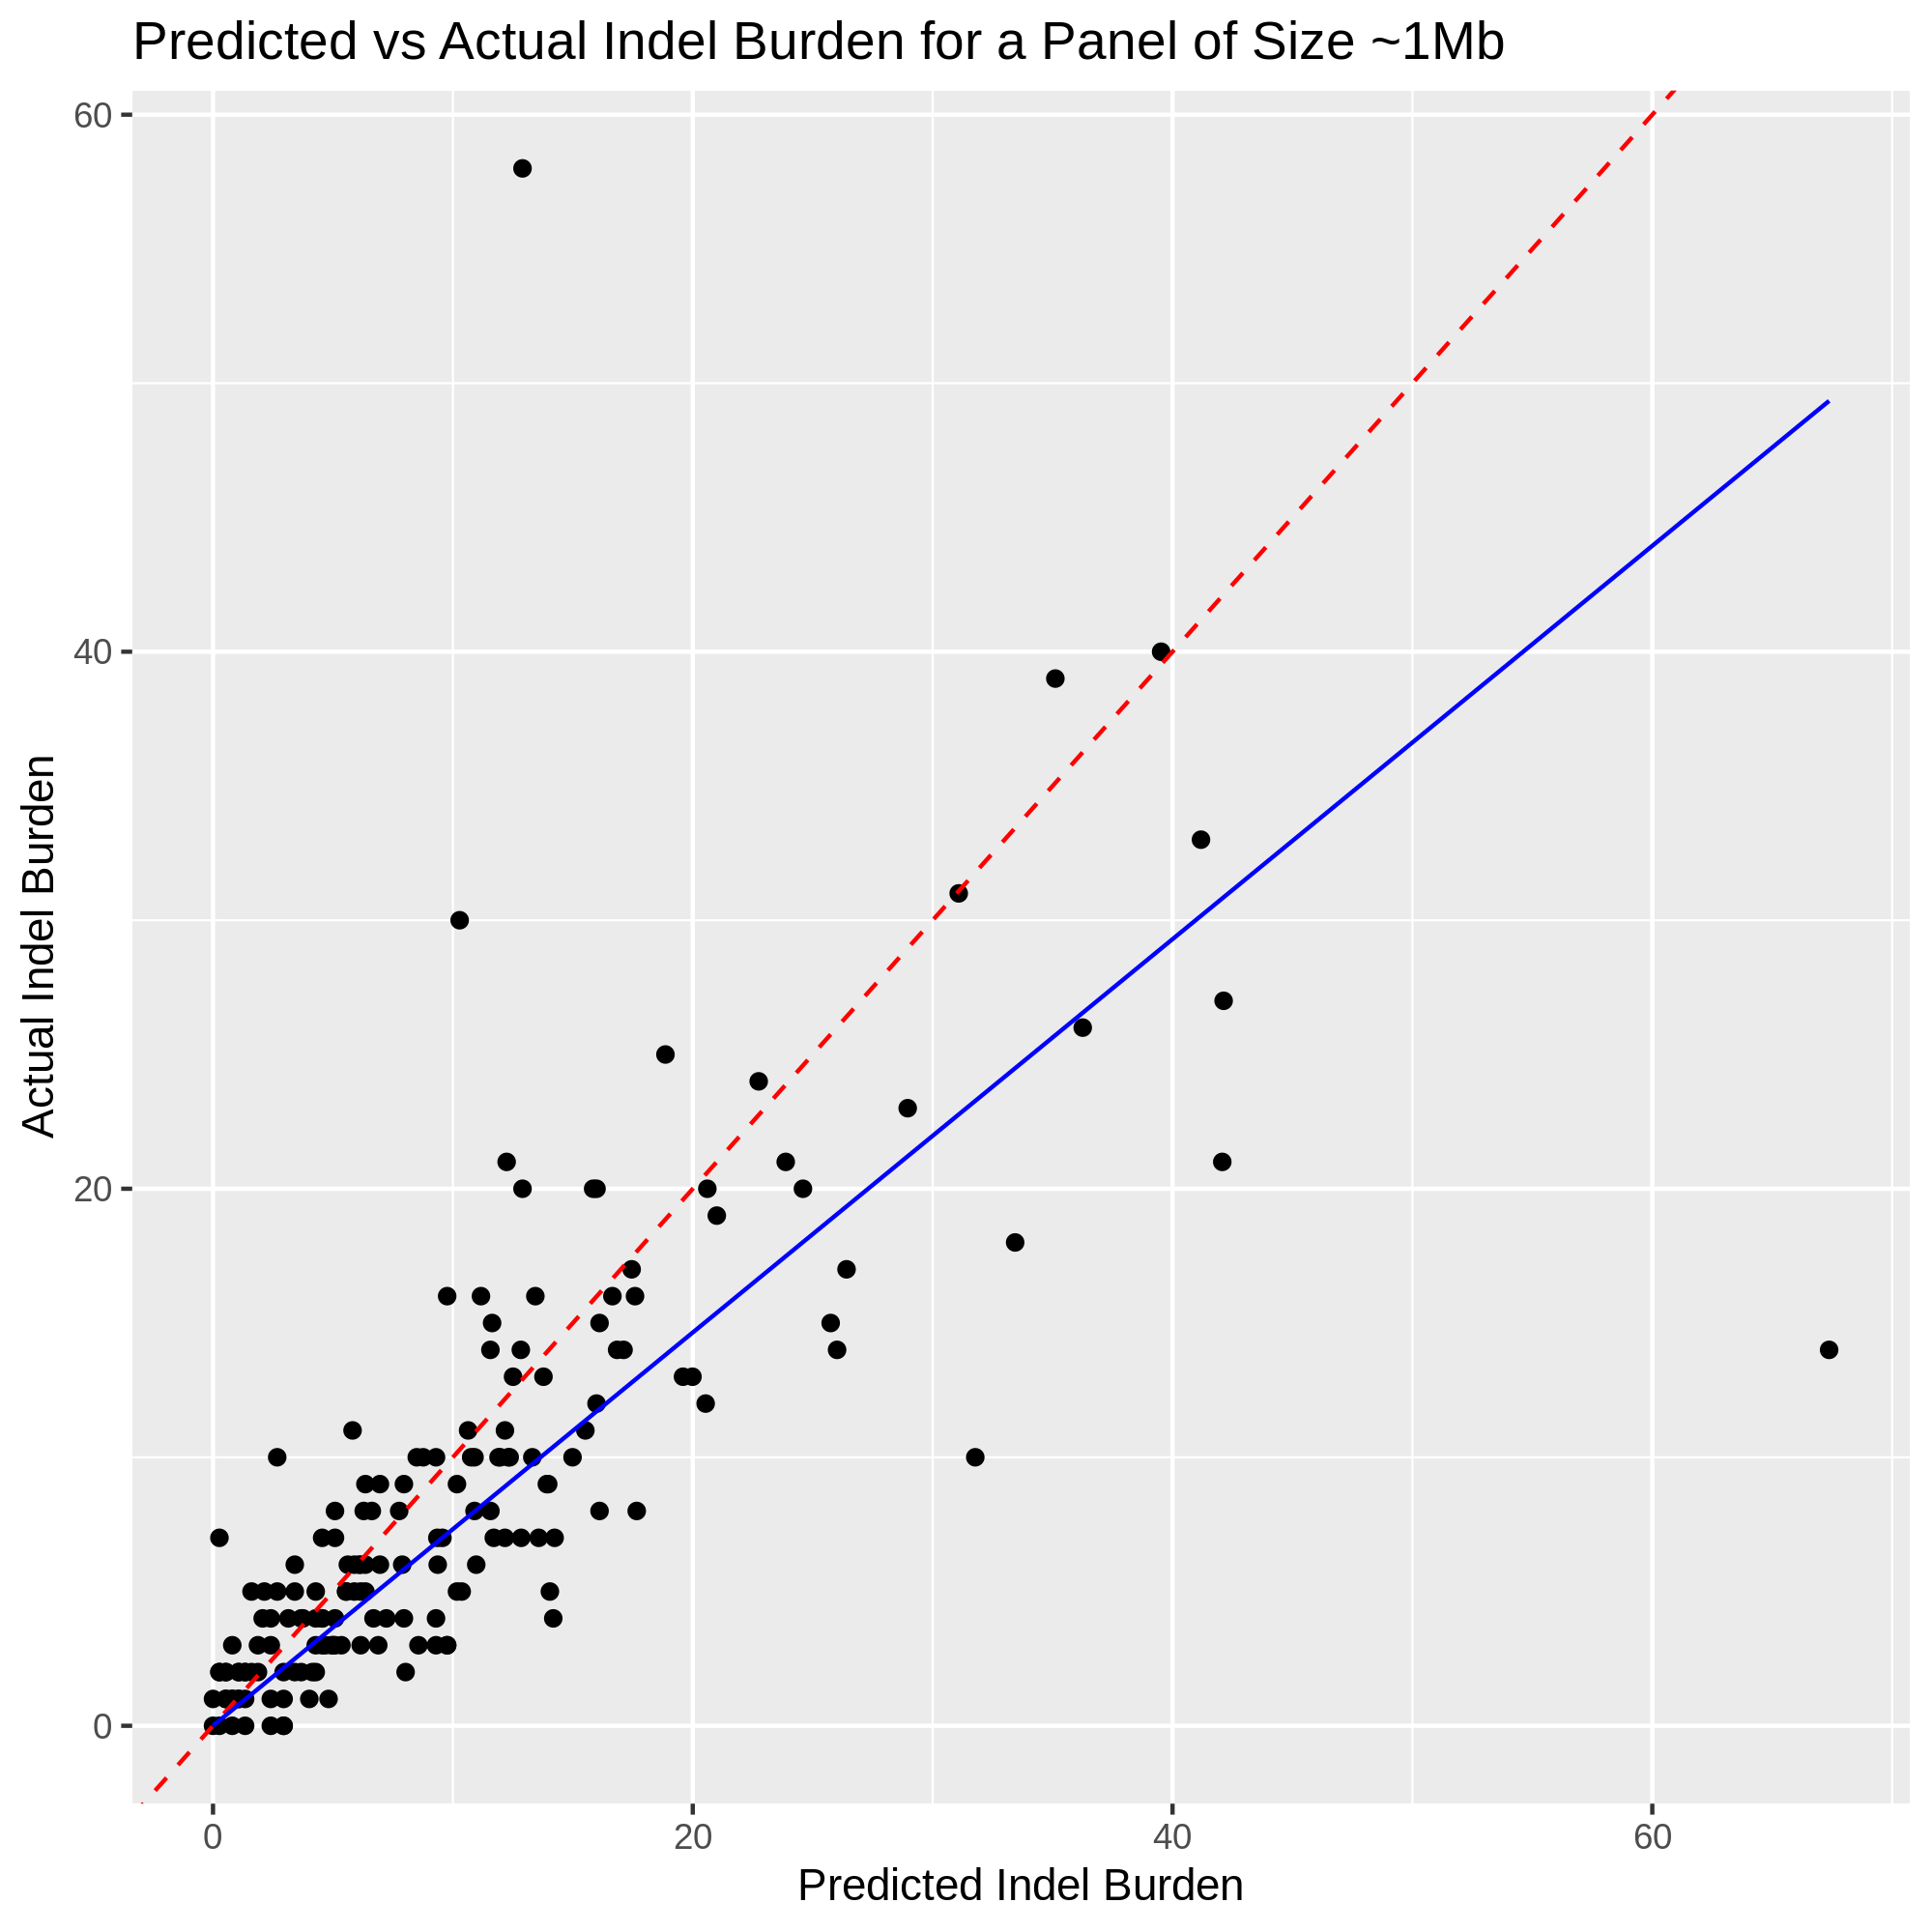
\includegraphics[width=4in]{indel_example.png}
% \caption{For a panel selected to be less than 1Mb in length, taken from the same validation set results as Figure \ref{fig:indelstatsplot}, we directly show predictions vs actual indel burden alongside intercept-free line of best fit. \label{fig:indelexample}}
% \end{figure}





% \begin{figure}[htbp]
% \centering
% 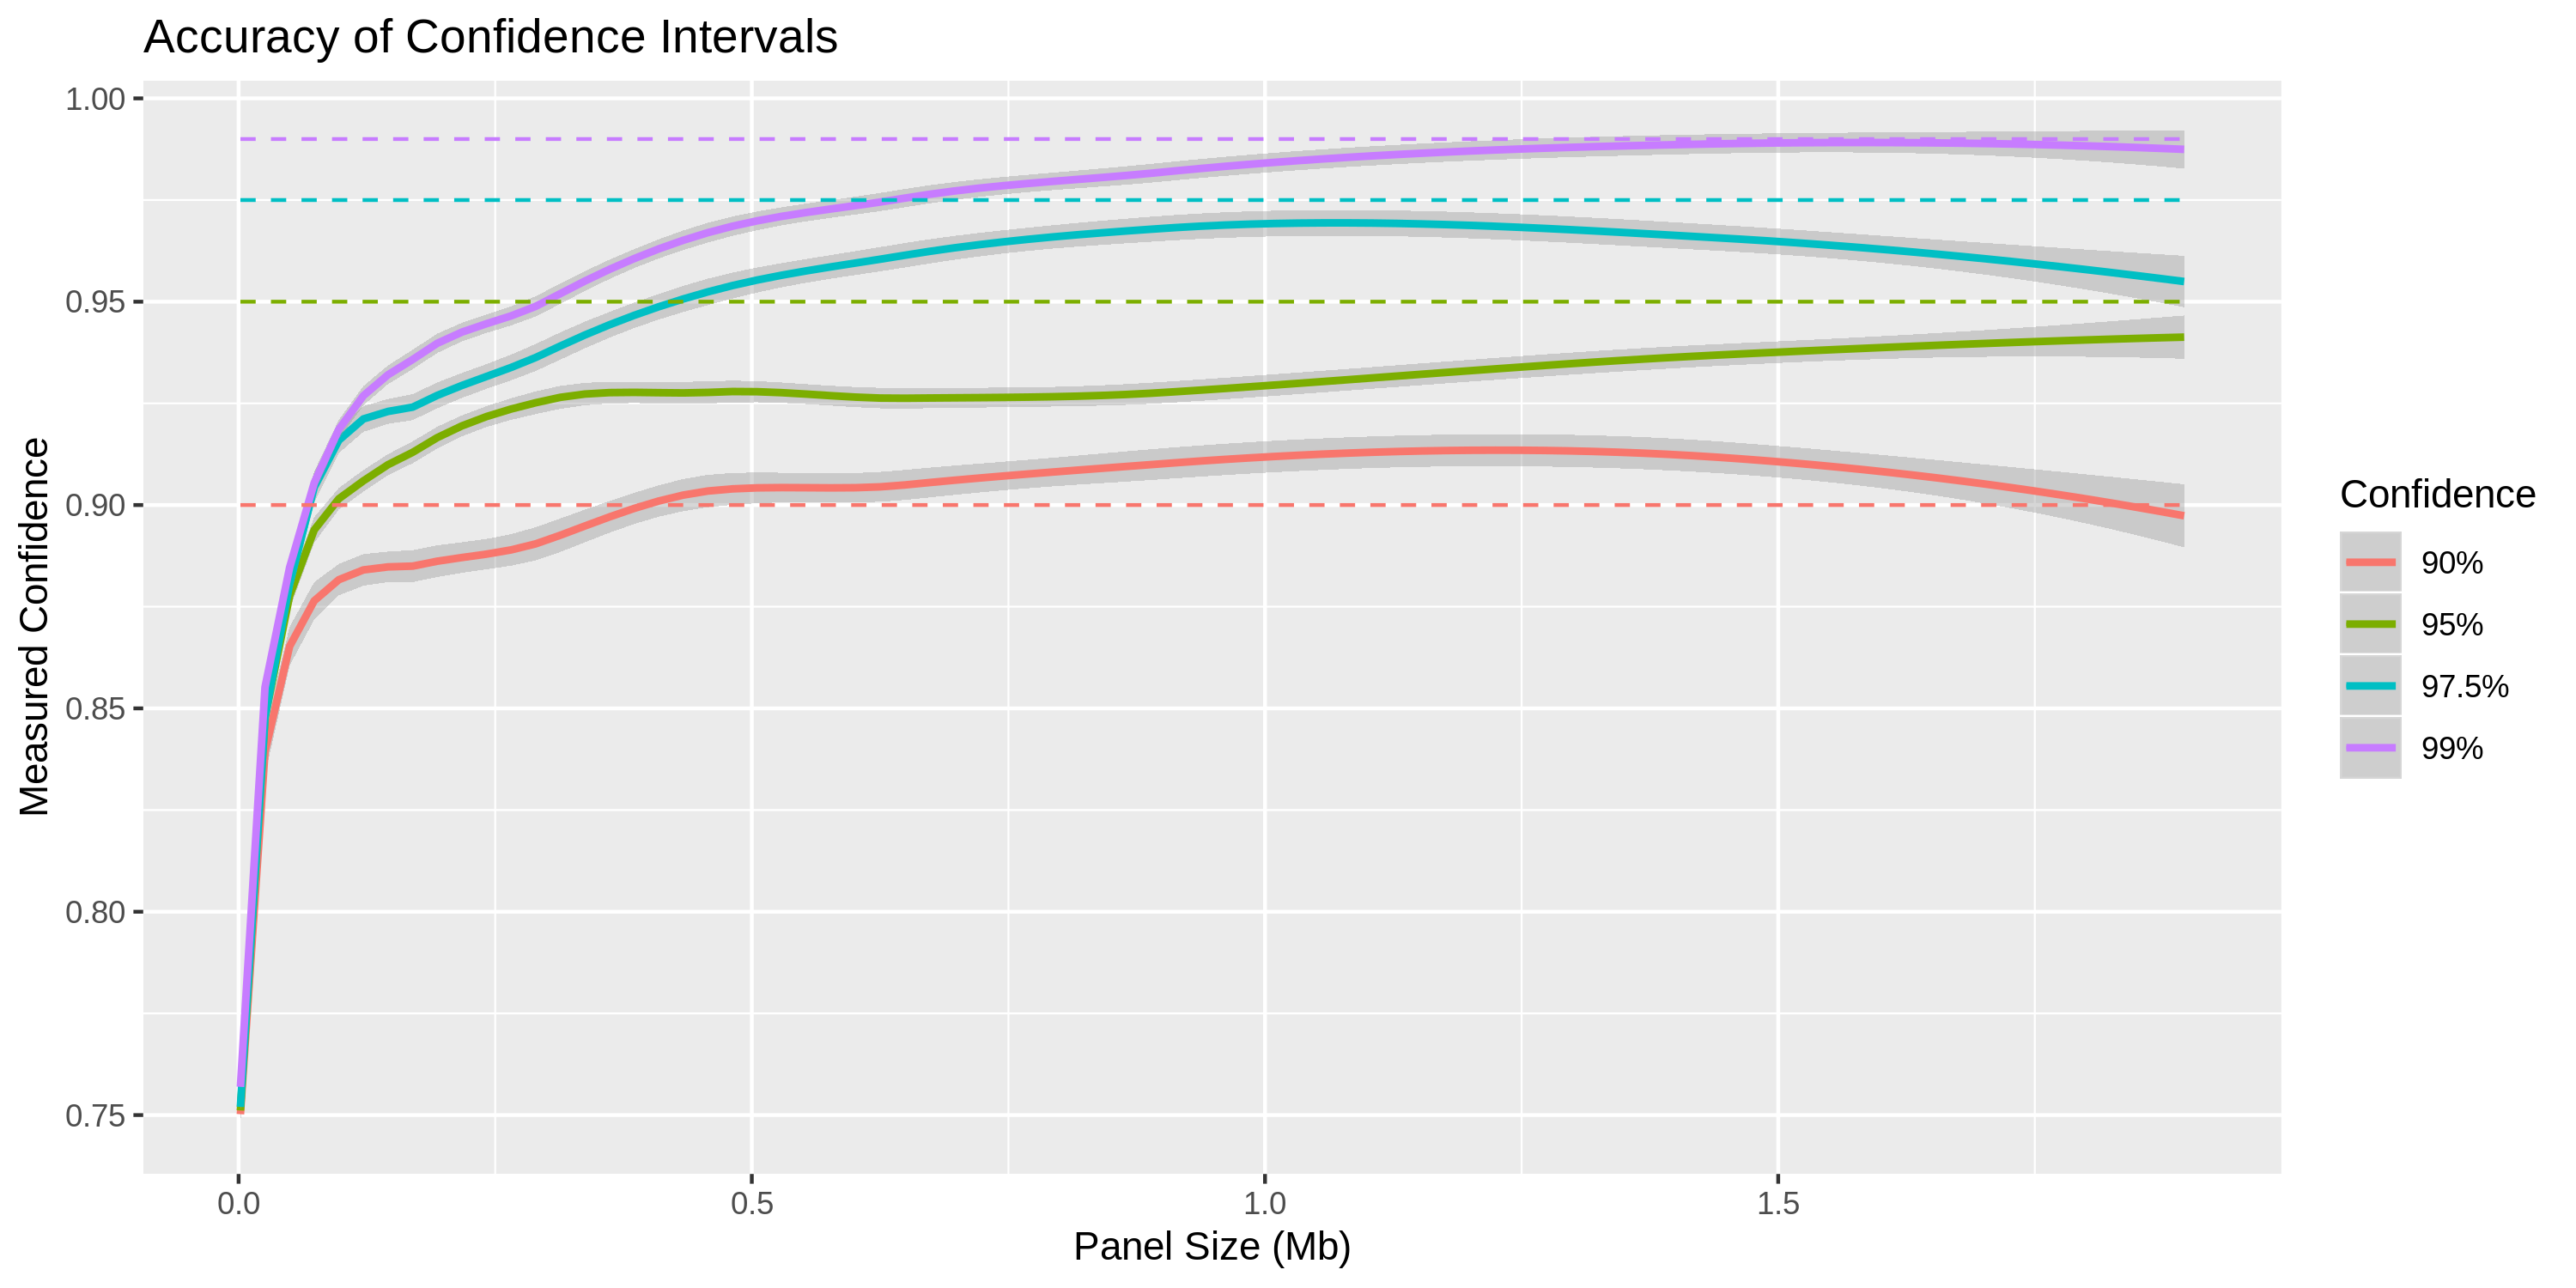
\includegraphics[width=6in]{ConfidencePlot.png}
% \caption{ \label{fig:confidenceplot}}
% \end{figure} 

% \section{Theoretical and Simulation Results \label{sec:theoreticalresults}}

% \subsection{Model Misspecification}
% \jbnote{While we don't observe overdispersion (quite the opposite), people do talk about it in the literature. We could write down a) a negative binomial and/or b) a quasi-poisson model and see whether we can derive any guarantees about the performance of our method.} Citation: \citep{martincorena_universal_2017}.


\section{Conclusions \label{sec:conclusion}}

 We have introduced a new data-driven framework for designing targeted gene panels which allows for cost-effective estimation of exome-wide biomarkers, such as \acrlong{tmb} and \acrlong{tib}.  Using the \acrshort{nsclc} dataset of \citet{campbell_distinct_2016}, we have demonstrated the excellent predictive performance of our proposal, and shown that it outperforms the existing state-of-the-art procedures. Our framework can be applied to any tumour dataset containing annotated mutations; we provide an \texttt{R} package \citep{BradleyCannings_2020} which implements the methodology.
 
The parameters of our fitted generative model in Section~\ref{sec:genmodelfit} also have interesting interpretations. For instance, of the five genes highlighted in Figure~\ref{fig:manhat_plot} as having the highest mutation rates relative to the \acrshort{bmr}, three (\textit{TP53, KRAS, CDKN2A}) are known tumour suppressors \citep{olivier_tp53_2010, jancik_clinical_2010, foulkes_cdkn2a_1997}.  Furthermore, indel mutations in \textit{KRAS} are known to be deleterious for tumour cells \citep{lee_selective_2018}, and this corresponds to the large negative indel-specific coefficient seen in Figure~\ref{fig:manhat_plot_indel}.  Our methodology identifies a number of other genes with particularly large parameter estimates, and further investigation into the biological relevance of this would be interesting in future studies.  

Finally, we believe there are many ways in which the general framework introduced in this paper could be extended. For example, it may adapted to incorporate alternate data types (e.g.~transcriptomics); alternatively we may seek to directly predict other outcomes (e.g.~patient survival) rather than intermediary biomarkers. 

%We present the fitted parameters of the model in Figures \ref{fig:manhat_plot} and \ref{fig:manhat_plot_indel}, where for each we have highlighted. Unsurprisingly, of the five genes with the largest positive coefficients, three (\textit{TP53, KRAS, CDKN2A}) are known tumour suppressors \citep{olivier_tp53_2010, jancik_clinical_2010, foulkes_cdkn2a_1997} and the remaining two (\textit{REG3A, REG1B}) belong to a family with multiple cancer-relevant interactions \citep{chen_four_2019}. Indel mutations in \textit{KRAS} are known to be deleterious for tumour cells, and this in itself is a target for precision gene-editing therapy \citep{lee_selective_2018}. There are many interesting biological interpretations associated with the genes highlighted in Figures~\ref{fig:manhat_plot} and \ref{fig:manhat_plot_indel}; see Section \ref{sec:??}.

%  We also show promise for estimating other biomarkers such as tumour indel burden, a problem for which no substantial body of work currently exists. 
%  These biomarkers are useful for identifying patients who might benefit from immunotherapy, but as of yet techniques for their estimation that are efficient enough to be viable have not been shown to be sufficiently reliable to make the transition to the clinic and a key concern of practitioners remains the confidence they can expect to have in the predictions being made. 
%  By grounding our predictive architecture in a generative model of mutation we are able to provide justification for including genes in predictive panels that have previously been excluded, as well as useful practical bounds for the error of our predictions. 
 
 %. We were able through optimised sparsity regularisation of our generative model to identify a large subset of genes following approximately the same mutation rate.  The notion of a background mutation rate has typically been used as a starting assumption for modelling work, rather than a quantified inference.  We were also able to identify genes showing particularly strong positive and negative selection for indel mutations, which in at least one case corresponded directly to an observation at the center of ongoing work on potential cancer therapies. 
 
% We see the key contribution of our work not as the performance of our method on the dataset with which we have demonstrated it, but rather its flexibility and broad applicability. There continues to be a large amount of research into immunosurveilling targeted gene panels, with many individual proposal panels presented each year. We have not produced such a panel beyond as a demonstration, but instead have designed our workflow to be as applicable to as broad a range of situations as possible. Our methodology can be used by those with a pre-defined gene panel or by those designing a new panel, either from scratch or augmenting on a starting set of targets. It is flexible in the sense that it can be used to predict biomarkers based on any set of mutation types. This will hopefully allow for further investigation into the utility of tumour indel burden, as well as being robust to changing standards of what genes and mutation types to include when reporting the more established biomarker of tumour mutation burden.
 
 
%  Furthermore statistical questions about goodness-of-fit of mutation models translate very naturally into biological questions about to the identification of cancer driver genes.   
 
% \subsection{Future work \label{sec:futurework}}
% While we have demonstrated good performance via a variety of benchmarks on one dataset, it remains to see whether similar performance can be achieved in other cancer types. Beyond this it remains an open (and controversial) question whether pan-cancer prognostic panels can be successful.

% Our methodology is designed to sample mutation density from a set of locations which minimises the cost of measurement. We do not allow in our model any causal interaction between mutations in one gene and mutations in another - all joint effects are mediated by a single sample-specific parameter. This appears to work well for prediction purposes, but does not allow us to ask questions about the genetic mechanisms of genomic instability, such as mismatch repair deficiency. A natural extension to our generative model would be to relax the condition of independence between mutation counts in a sample. This could be done in a variety of ways, including via causal networks. The main challenge here is the explosion of complexity with dimensionality when fitting large directed acyclic graphs. If these issues could be overcome, it would provide the scope to ask a large class of questions about the molecular origins of hypermutated tumours.

% As the field progresses, biomarkers such as tumour mutation burden may be replaceable by more finely tuned biomarkers. As a crude proxy for neoantigen burden, which is in itself only one factor modulating response to immunotherapy, tumour mutation burden has shown great utility and broken several barriers, including being the first exome-wide biomarker to be approved as a companion prognostic for a class of cancer drugs regardless of a tumour's tissue of origin. However, it remains limited by a number of factors. Only mutations which are expressed get the chance to form neoantigens, and so integrating information about the transcriptomic profile of tumours via gene expression profiling is a promising first step towards more nuanced, multi-omic biomarkers. Additionally, the differing immunogenicity of mutation types is not fully understood. The ability to predict the indel constitution of a tumour's mutation profile, as we have shown here, is a good first step, but is only as useful as the meaningful clinical consequences that can be derived from it.
% \subsection{Other applications}
% Our methods are broadly applicable in any area for which an estimate of some total population is required from expensive subsampling. Examples of such problems include the analysis of polling data, estimating the usage of transport networks, and destructive testing of manufactured goods. 


\section{Acknowledgements}
We gratefully acknowledge funding provided by Cambridge Cancer Genomics (CCG) through their PhD Scholarship at the University of Edinburgh. We also benefited from discussions with several individuals, including Adnan Akbar, Philip Beer, Harry Clifford, Aleksandra Jartseva, Morton, Kevin Myant, William Orchard, Nirmesh Patel and Charlotte Paterson.

\bibliography{zotero-refs.bib}
% \section*{Appendices}
% \appendix
% \section{Genes Experiencing Strong Selection for Indel Mutations \label{appendix:indelselection}}
% We give in Table \ref{table:indelselection} the genes for which we recovered the strongest positive or negative interaction term for indel mutations, i.e. those which show the strongest signs of positive or negative selection for indel mutations relative to other mutation types. Quoted $p$-values are given by the method of post-selective inference for generalised linear models described by \citet{taylor_post-selection_2018} \jbnote{Not yet they're not}. Negative selection may indicate that genes bearing indel mutations lead to less viable tumour cells. The gene showing the strongest negative selection is \textit{KRAS}, a well-known oncogene and frequent (if formidable) target for pipeline therapeutics \citep{mullard_cracking_2019}. Indel mutations in \textit{KRAS} are known to be deleterious for tumour cells, and this in itself is a target for precision gene-editing therapy \citep{lee_selective_2018}.

% \begin{table}
% \begin{center}
% % \begin{tabular}{ || c | c | c|| c | c | c ||}
% \begin{tabular}{ || c | c || c | c ||}
% \hline
% \hline
% % \multicolumn{4}{||c||c||}{Country List} \\
% \multicolumn{2}{||c||}{Positive Indel Selection} & \multicolumn{2}{c||}{Negative Indel Selection} \\

% % \multicolumn{3}{||c||}{Positive Indel Selection} & \multicolumn{3}{c||}{Negative Indel Selection} \\

% \hline 
% \hline
% % Gene Symbol  &  $\eta_{g,\mathrm{indel}}$  & $p$-value &  Gene Symbol & $\eta_{g,\mathrm{indel}}$ & $p$-value \\
% Gene Symbol  &  $\eta_{g,\mathrm{indel}}$   &  Gene Symbol & $\eta_{g,\mathrm{indel}}$  \\
% \hline
% \hline
% \textit{RPL41} & 3.82 &  \textit{KRAS}& -2.91  \\
% \textit{CKS2} &3.67 &  \textit{REG3A} & -1.73  \\
% \textit{CDKN1B} &3.44  & \textit{SORCS1} & -1.69  \\
% \textit{TNFRSF10C} & 3.45 & \textit{OR4M2} & -1.65  \\
% \textit{SPCS1} &3.34 &\textit{LRRTM4} & -1.63\\
% \textit{MT1G} &3.16 &\textit{EGFR} & - 1.54\\
% \textit{SUMO1} &3.02  &\textit{ZIC1} & -1.54\\
% \textit{GNG12} &2.96  &\textit{TRIM58} & -1.51 \\
% \textit{SPRR2F} &2.96 &\textit{NFE2L2} & -1.39\\
% \textit{AANAT} &2.92 &\textit{CNTNAP4} & -1.37\\

% \hline
% \hline
% \end{tabular}
% \end{center}
% \caption{Genes with maximum positive and negative selection for indel mutations.\label{table:indelselection}}
% \end{table}

% \section{Goodness-of-Fit Testing to Identify Driver Regions\label{app:goodnessoffit}}
% Goodness-of-fit tests based on flexible regression of residuals have been proposed recently for high-dimensional linear models \citep{shah_goodness_2018} and generalised linear models \citep{jankova_goodness--fit_2019}. We hope that it will be possible to use these to further validate our generative model. In particular, learning a flexible regression model to predict the residual errors of our model could help us understand in what genomic locations mutations deviate most from our Poisson assumptions. This could be used as a method for identifying genes with hotspot driver codons, which will likely have mutation counts more closely grouped around their mean than predicted by the learned model.




% \section{Formal Error Bounds \label{app:errorbounds}}
% \subsection{Oracle Error Bound}
% We first study the case when the true generative model is known, and begin by constructing a bound on the error of our estimate of the form $\tau + \epsilon\hat{T}$ ($\tau$, $\epsilon$ constants). We can form a Chernoff-style lower bound by noting that
% \[
% \mathbb{P}(\hat{T} - T_{\bar{S}} \geq \tau_- + \epsilon_-\hat{T}) \leq \mathbb{E}[\exp(\theta ( -\tau_-  + \hat{T}(1- \epsilon_-) - T_{\bar{S}}))] 
% \]
% \[ 
% = \exp \big(-\theta \tau_- + e^{\mu}\sum_{g,s}\phi_{gs}(e^{\theta w_{gs}(1-\epsilon_- ) - \theta} - 1) \big)  \quad \mathrm{for \ any \ } \theta > 0.
% \]
% where $\phi_{gs} = \exp(\log(\ell_g) + \lambda_{gs})$ is the gene/mutation type component of the mutation rate $\phi_{gs}$. It is undesirable that this depends on $e^{\mu}$, so we will always choose $\epsilon_-$ such that $\sum_{g,s}\phi_{gs}(e^{\theta w_{gs}(1-\epsilon) - \theta} - 1) = 0$. Therefore, for a value $q \in [0,1]$, we have a set of pairs $(\tau_-(\theta; q), \epsilon_-(\theta))$ parameterised by $\theta$ via
% \[\tau_-(\theta; q) = \frac{-\log(q)}{\theta}, \quad \epsilon_-(\theta) = \argmin\limits_{\epsilon > 0} \big| \sum_{g,s}\phi_{gs}(e^{\theta w_{gs}(1-\epsilon) -  \theta }-1) \big|. \]
% To construct an upper bound we perform a similar process to obtain a family $(\tau_+(\theta;q), \epsilon_+(\theta))$. We may then say that
% \[
% \mathbb{P} \big(\max\limits_{\theta_1>0}\{-\tau_-(\theta_1;\frac{q}{2}) + (1-\epsilon_-(\theta_1))\hat{T}\} \leq T_{\bar{S}} \leq \min\limits_{\theta_2 > 0} \{ \tau_+(\theta_2;\frac{q}{2}) + (1+\epsilon_+(\theta_2))\hat{T}\} \big) \geq 1-q,
% \]
% giving us a bound on $T_{\bar{S}}$ that depends only on the generative model parameters $\phi_{gs}$ and the coefficients $w_{gs}$ of our proposed linear estimator.
% \subsection{Incorporating Generative Model Error}
% We may not assume that the parameter estimates of our generative model are asymptotically normally distributed, because of the sparsity penalty employed in their fitting. We hopefully however can use the methodology of \citet{taylor_post-selection_2018} to produce confidence intervals for the generative model parameters. We then may take the most extreme values of these parameters to produce confidence intervals.


\end{document}